% Options for packages loaded elsewhere
\PassOptionsToPackage{unicode}{hyperref}
\PassOptionsToPackage{hyphens}{url}
\PassOptionsToPackage{dvipsnames,svgnames,x11names}{xcolor}
%
\documentclass[
]{book}
\usepackage{amsmath,amssymb}
\usepackage{lmodern}
\usepackage{iftex}
\ifPDFTeX
  \usepackage[T1]{fontenc}
  \usepackage[utf8]{inputenc}
  \usepackage{textcomp} % provide euro and other symbols
\else % if luatex or xetex
  \usepackage{unicode-math}
  \defaultfontfeatures{Scale=MatchLowercase}
  \defaultfontfeatures[\rmfamily]{Ligatures=TeX,Scale=1}
\fi
% Use upquote if available, for straight quotes in verbatim environments
\IfFileExists{upquote.sty}{\usepackage{upquote}}{}
\IfFileExists{microtype.sty}{% use microtype if available
  \usepackage[]{microtype}
  \UseMicrotypeSet[protrusion]{basicmath} % disable protrusion for tt fonts
}{}
\makeatletter
\@ifundefined{KOMAClassName}{% if non-KOMA class
  \IfFileExists{parskip.sty}{%
    \usepackage{parskip}
  }{% else
    \setlength{\parindent}{0pt}
    \setlength{\parskip}{6pt plus 2pt minus 1pt}}
}{% if KOMA class
  \KOMAoptions{parskip=half}}
\makeatother
\usepackage{xcolor}
\usepackage{color}
\usepackage{fancyvrb}
\newcommand{\VerbBar}{|}
\newcommand{\VERB}{\Verb[commandchars=\\\{\}]}
\DefineVerbatimEnvironment{Highlighting}{Verbatim}{commandchars=\\\{\}}
% Add ',fontsize=\small' for more characters per line
\usepackage{framed}
\definecolor{shadecolor}{RGB}{248,248,248}
\newenvironment{Shaded}{\begin{snugshade}}{\end{snugshade}}
\newcommand{\AlertTok}[1]{\textcolor[rgb]{0.33,0.33,0.33}{#1}}
\newcommand{\AnnotationTok}[1]{\textcolor[rgb]{0.37,0.37,0.37}{\textbf{\textit{#1}}}}
\newcommand{\AttributeTok}[1]{\textcolor[rgb]{0.61,0.61,0.61}{#1}}
\newcommand{\BaseNTok}[1]{\textcolor[rgb]{0.06,0.06,0.06}{#1}}
\newcommand{\BuiltInTok}[1]{#1}
\newcommand{\CharTok}[1]{\textcolor[rgb]{0.5,0.5,0.5}{#1}}
\newcommand{\CommentTok}[1]{\textcolor[rgb]{0.37,0.37,0.37}{\textit{#1}}}
\newcommand{\CommentVarTok}[1]{\textcolor[rgb]{0.37,0.37,0.37}{\textbf{\textit{#1}}}}
\newcommand{\ConstantTok}[1]{\textcolor[rgb]{0,0,0}{#1}}
\newcommand{\ControlFlowTok}[1]{\textcolor[rgb]{0.27,0.27,0.27}{\textbf{#1}}}
\newcommand{\DataTypeTok}[1]{\textcolor[rgb]{0.27,0.27,0.27}{#1}}
\newcommand{\DecValTok}[1]{\textcolor[rgb]{0.06,0.06,0.06}{#1}}
\newcommand{\DocumentationTok}[1]{\textcolor[rgb]{0.37,0.37,0.37}{\textbf{\textit{#1}}}}
\newcommand{\ErrorTok}[1]{\textcolor[rgb]{0.14,0.14,0.14}{\textbf{#1}}}
\newcommand{\ExtensionTok}[1]{#1}
\newcommand{\FloatTok}[1]{\textcolor[rgb]{0.06,0.06,0.06}{#1}}
\newcommand{\FunctionTok}[1]{\textcolor[rgb]{0,0,0}{#1}}
\newcommand{\ImportTok}[1]{#1}
\newcommand{\InformationTok}[1]{\textcolor[rgb]{0.37,0.37,0.37}{\textbf{\textit{#1}}}}
\newcommand{\KeywordTok}[1]{\textcolor[rgb]{0.27,0.27,0.27}{\textbf{#1}}}
\newcommand{\NormalTok}[1]{#1}
\newcommand{\OperatorTok}[1]{\textcolor[rgb]{0.43,0.43,0.43}{\textbf{#1}}}
\newcommand{\OtherTok}[1]{\textcolor[rgb]{0.37,0.37,0.37}{#1}}
\newcommand{\PreprocessorTok}[1]{\textcolor[rgb]{0.37,0.37,0.37}{\textit{#1}}}
\newcommand{\RegionMarkerTok}[1]{#1}
\newcommand{\SpecialCharTok}[1]{\textcolor[rgb]{0,0,0}{#1}}
\newcommand{\SpecialStringTok}[1]{\textcolor[rgb]{0.5,0.5,0.5}{#1}}
\newcommand{\StringTok}[1]{\textcolor[rgb]{0.5,0.5,0.5}{#1}}
\newcommand{\VariableTok}[1]{\textcolor[rgb]{0,0,0}{#1}}
\newcommand{\VerbatimStringTok}[1]{\textcolor[rgb]{0.5,0.5,0.5}{#1}}
\newcommand{\WarningTok}[1]{\textcolor[rgb]{0.37,0.37,0.37}{\textbf{\textit{#1}}}}
\usepackage{longtable,booktabs,array}
\usepackage{calc} % for calculating minipage widths
% Correct order of tables after \paragraph or \subparagraph
\usepackage{etoolbox}
\makeatletter
\patchcmd\longtable{\par}{\if@noskipsec\mbox{}\fi\par}{}{}
\makeatother
% Allow footnotes in longtable head/foot
\IfFileExists{footnotehyper.sty}{\usepackage{footnotehyper}}{\usepackage{footnote}}
\makesavenoteenv{longtable}
\usepackage{graphicx}
\makeatletter
\def\maxwidth{\ifdim\Gin@nat@width>\linewidth\linewidth\else\Gin@nat@width\fi}
\def\maxheight{\ifdim\Gin@nat@height>\textheight\textheight\else\Gin@nat@height\fi}
\makeatother
% Scale images if necessary, so that they will not overflow the page
% margins by default, and it is still possible to overwrite the defaults
% using explicit options in \includegraphics[width, height, ...]{}
\setkeys{Gin}{width=\maxwidth,height=\maxheight,keepaspectratio}
% Set default figure placement to htbp
\makeatletter
\def\fps@figure{htbp}
\makeatother
\setlength{\emergencystretch}{3em} % prevent overfull lines
\providecommand{\tightlist}{%
  \setlength{\itemsep}{0pt}\setlength{\parskip}{0pt}}
\setcounter{secnumdepth}{5}
\usepackage{booktabs}
%These packages added to resolve tex problems arising from kable tables.
\usepackage{tabularx}
\usepackage{float}
%%
\usepackage{longtable}
\usepackage[bf,singlelinecheck=off]{caption}

\usepackage{framed,color}
\definecolor{shadecolor}{RGB}{248,248,248}

\renewcommand{\textfraction}{0.05}
\renewcommand{\topfraction}{0.8}
\renewcommand{\bottomfraction}{0.8}
\renewcommand{\floatpagefraction}{0.75}

%%%%%%%%
% Inserting new commands here


%%%%%%%%

%\renewenvironment{quote}{\begin{VF}}{\end{VF}}
%\let\oldhref\href
%\renewcommand{\href}[2]{#2\footnote{\url{#1}}}

\makeatletter
\newenvironment{kframe}{%
\medskip{}
\setlength{\fboxsep}{.8em}
 \def\at@end@of@kframe{}%
 \ifinner\ifhmode%
  \def\at@end@of@kframe{\end{minipage}}%
  \begin{minipage}{\columnwidth}%
 \fi\fi%
 \def\FrameCommand##1{\hskip\@totalleftmargin \hskip-\fboxsep
 \colorbox{shadecolor}{##1}\hskip-\fboxsep
     % There is no \\@totalrightmargin, so:
     \hskip-\linewidth \hskip-\@totalleftmargin \hskip\columnwidth}%
 \MakeFramed {\advance\hsize-\width
   \@totalleftmargin\z@ \linewidth\hsize
   \@setminipage}}%
 {\par\unskip\endMakeFramed%
 \at@end@of@kframe}
\makeatother

% This change to the shaded environment adapted from https://github.com/yihui/bookdown-chinese/commit/a3e392593b464ba31a7eceb0cd60f7e0bd112798 and https://stackoverflow.com/questions/41052687/rstudio-pdf-knit-fails-with-environment-shaded-undefined-error
\makeatletter
\@ifundefined{Shaded}{
}{\renewenvironment{Shaded}{\begin{kframe}}{\end{kframe}}}
\makeatother

\usepackage{makeidx}
\makeindex

%\urlstyle{tt}

\usepackage{amsthm}
\makeatletter
\def\thm@space@setup{%
  \thm@preskip=8pt plus 2pt minus 4pt
  \thm@postskip=\thm@preskip
}
\makeatother

\frontmatter
\usepackage{booktabs}
\usepackage{longtable}
\usepackage{array}
\usepackage{multirow}
\usepackage{wrapfig}
\usepackage{float}
\usepackage{colortbl}
\usepackage{pdflscape}
\usepackage{tabu}
\usepackage{threeparttable}
\usepackage{threeparttablex}
\usepackage[normalem]{ulem}
\usepackage{makecell}
\usepackage{xcolor}
\ifLuaTeX
  \usepackage{selnolig}  % disable illegal ligatures
\fi
\usepackage[]{natbib}
\bibliographystyle{plainnat}
\IfFileExists{bookmark.sty}{\usepackage{bookmark}}{\usepackage{hyperref}}
\IfFileExists{xurl.sty}{\usepackage{xurl}}{} % add URL line breaks if available
\urlstyle{same} % disable monospaced font for URLs
\hypersetup{
  pdftitle={Chapter 2},
  pdfauthor={Raúl Alberto Pérez},
  colorlinks=true,
  linkcolor={Maroon},
  filecolor={Maroon},
  citecolor={Blue},
  urlcolor={Blue},
  pdfcreator={LaTeX via pandoc}}

\title{Chapter 2}
\usepackage{etoolbox}
\makeatletter
\providecommand{\subtitle}[1]{% add subtitle to \maketitle
  \apptocmd{\@title}{\par {\large #1 \par}}{}{}
}
\makeatother
\subtitle{Distribución Normal Multivariada}
\author{Raúl Alberto Pérez}
\date{diciembre 14, 2022}

\usepackage{amsthm}
\newtheorem{theorem}{Teorema}[chapter]
\newtheorem{lemma}{Lema}[chapter]
\newtheorem{corollary}{Corolario}[chapter]
\newtheorem{proposition}{Proposición}[chapter]
\newtheorem{conjecture}{Conjecture}[chapter]
\theoremstyle{definition}
\newtheorem{definition}{Definición}[chapter]
\theoremstyle{definition}
\newtheorem{example}{Ejemplo}[chapter]
\theoremstyle{definition}
\newtheorem{exercise}{Ejercicio}[chapter]
\theoremstyle{definition}
\newtheorem{hypothesis}{Hypothesis}[chapter]
\theoremstyle{remark}
\newtheorem*{remark}{Observación}
\newtheorem*{solution}{Solución}
\begin{document}
\maketitle

% you may need to leave a few empty pages before the dedication page

%\cleardoublepage\newpage\thispagestyle{empty}\null
%\cleardoublepage\newpage\thispagestyle{empty}\null
%\cleardoublepage\newpage
\thispagestyle{empty}

\setlength{\abovedisplayskip}{-5pt}
\setlength{\abovedisplayshortskip}{-5pt}

{
\hypersetup{linkcolor=}
\setcounter{tocdepth}{2}
\tableofcontents
}
\hypertarget{prefacio}{%
\chapter*{Prefacio}\label{prefacio}}


\textbf{Introducción al Análisis Multivariado} se escribió con la intención de \ldots\ldots\ldots\ldots\ldots{} usando \citep{R-base} y además\ldots\ldots\ldots..

\textbf{Agradecimientos.} Quiero agradecer a mis compañeros de trabajo Victor López, \ldots\ldots\ldots..

\begin{Shaded}
\begin{Highlighting}[]
\CommentTok{\# R packages needed for this book}
\CommentTok{\#   along with versions used when book knitted in Jan 2021}

\CommentTok{\# Install CRAN packages needed}
\NormalTok{needed\_pkgs }\OtherTok{\textless{}{-}} \FunctionTok{c}\NormalTok{(}
  \StringTok{"bookdown"}\NormalTok{,     }\CommentTok{\# 0.19}
  \StringTok{"boot"}\NormalTok{,         }\CommentTok{\# 1.3{-}25}
  \StringTok{"broom"}\NormalTok{,        }\CommentTok{\# 0.5.6}
  \StringTok{"data.table"}\NormalTok{,   }\CommentTok{\# 1.12.8}
  \StringTok{"GGally"}\NormalTok{,       }\CommentTok{\# 2.0.0}
  \StringTok{"ggmosaic"}\NormalTok{,     }\CommentTok{\# 0.2.0}
  \StringTok{"gridExtra"}\NormalTok{,    }\CommentTok{\# 2.3}
  \StringTok{"Hmisc"}\NormalTok{,        }\CommentTok{\# 4.4{-}0}
  \StringTok{"HMLdiag"}\NormalTok{,      }\CommentTok{\# 0.3.1}
  \StringTok{"ICC"}\NormalTok{,          }\CommentTok{\# 2.3.0}
  \StringTok{"jtools"}\NormalTok{,       }\CommentTok{\# 2.0.5}
  \StringTok{"kableExtra"}\NormalTok{,   }\CommentTok{\# 1.1.0}
  \StringTok{"knitr"}\NormalTok{,        }\CommentTok{\# 1.28}
  \StringTok{"lattice"}\NormalTok{,      }\CommentTok{\# 0.20{-}41}
  \StringTok{"lme4"}\NormalTok{,         }\CommentTok{\# 1.1{-}23}
  \StringTok{"MASS"}\NormalTok{,         }\CommentTok{\# 7.3{-}51.6}
  \StringTok{"mice"}\NormalTok{,         }\CommentTok{\# 3.9.0}
  \StringTok{"mnormt"}\NormalTok{,       }\CommentTok{\# 2.0.0}
  \StringTok{"mosaic"}\NormalTok{,       }\CommentTok{\# 1.7.0}
  \StringTok{"multcomp"}\NormalTok{,     }\CommentTok{\# 1.4{-}13}
  \StringTok{"nlme"}\NormalTok{,         }\CommentTok{\# 3.1{-}148}
  \StringTok{"pander"}\NormalTok{,       }\CommentTok{\# 0.6.3}
  \StringTok{"pscl"}\NormalTok{,         }\CommentTok{\# 1.5.5}
  \StringTok{"reshape2"}\NormalTok{,     }\CommentTok{\# 1.4.4}
  \StringTok{"rsample"}\NormalTok{,      }\CommentTok{\# 0.0.7}
  \StringTok{"sessioninfo"}\NormalTok{,  }\CommentTok{\# 1.1.1}
  \StringTok{"tidyverse"}\NormalTok{,    }\CommentTok{\# 1.3.0}
  \StringTok{"xtable"}        \CommentTok{\# 1.8{-}4}
\NormalTok{)}

\DocumentationTok{\#\# Automatically installing needed packages not yet installed}
\CommentTok{\#new\_pkgs \textless{}{-} needed\_pkgs[!(needed\_pkgs \%in\%}
\CommentTok{\#  installed.packages())]}
\CommentTok{\#if (length(new\_pkgs)) \{}
\CommentTok{\#  install.packages(new\_pkgs, repos = "http://cran.rstudio.com")}
\CommentTok{\#\}}
\end{Highlighting}
\end{Shaded}

\begin{Shaded}
\begin{Highlighting}[]
\ControlFlowTok{if}\NormalTok{(knitr}\SpecialCharTok{::}\FunctionTok{is\_html\_output}\NormalTok{())\{}\FunctionTok{options}\NormalTok{(}\AttributeTok{knitr.table.format =} \StringTok{"html"}\NormalTok{)\} }\ControlFlowTok{else}\NormalTok{ \{}\FunctionTok{options}\NormalTok{(}\AttributeTok{knitr.table.format =} \StringTok{"latex"}\NormalTok{)\}}
\end{Highlighting}
\end{Shaded}

\mainmatter

\hypertarget{rep_al}{%
\chapter{Repaso de álgebra lineal}\label{rep_al}}

\newcommand{\xdatos}{\mathbf{X}_{n\times p}=\begin{bmatrix}
x_{11} & x_{12} & \cdots & x_{1p}\\
x_{21} & x_{22} & \cdots & x_{2p}\\
\vdots & \vdots & & \vdots \\
x_{n1} & x_{n2} & \cdots & x_{np}
\end{bmatrix}}

\newcommand{\vecmu}{
{\large \underline{\mathbf{\mu}}}\ }

\newcommand{\sumasx}{\begin{bmatrix}
\sum_{i=1}^n x_{i1}\\
\sum_{i=1}^n x_{i2}\\
\vdots  \\
\sum_{i=1}^n x_{ip}
\end{bmatrix}}

\newcommand{\xvector}{\begin{bmatrix}
X_1 \\ X_2 \\ \vdots \\ X_p
\end{bmatrix}}

\newcommand{\smuestral}{\begin{bmatrix}
s_{11} & s_{12} & \cdots & s_{1p}\\
s_{21} & s_{22} & \cdots & s_{2p}\\
\vdots & \vdots & \ddots & \vdots\\
s_{p1} & s_{p2} & \cdots & s_{pp}\\
\end{bmatrix}}

\hypertarget{algunos-conceptos-buxe1sicos}{%
\section{Algunos conceptos básicos}\label{algunos-conceptos-buxe1sicos}}

\begin{definition}[Vector]
\protect\hypertarget{def:vector}{}\label{def:vector}Arreglo de \(n\)-números reales
\end{definition}

\begin{definition}[Vector de Unos]
\protect\hypertarget{def:vector-unos}{}\label{def:vector-unos}Vector cuyas entradas son todos uno
\end{definition}

\begin{definition}[Suma de Vectores]
\protect\hypertarget{def:suma-vect}{}\label{def:suma-vect}Se realiza la suma componente a componente
\end{definition}

\begin{definition}[Producto interno entre vectores]
\protect\hypertarget{def:prod-inter}{}\label{def:prod-inter}Multiplicación elemento a elemento, ie.
\[
\langle \underline{a} \ , \ \underline{b} \rangle =a_1b_1+a_2b_2+\cdots+a_n b_n= \sum_i a_i b_i
\]
\end{definition}

\begin{definition}[Norma de un Vector]
\protect\hypertarget{def:norma-vect}{}\label{def:norma-vect}Es la raíz cuadrada del producto interno del vector por si mismo, ie.
\[
\|\underline{a} \|=\sqrt{\langle \underline{a}\ , \ \underline{a} \rangle}=\sqrt{\underline{a}^t\underline{a}}=\sqrt{a_1^2+a_2^2+\cdots+a_n^2},
\]
con \(\underline{a}^t=(a_1,a_2,\ldots,a_n)\)
\end{definition}

\textbf{Propiedades de la Norma:}

\(\|c \underline{a} \|=|c|\|\underline{a}\|\), si \(|c|>1\) entonces \(\underline{a}\)-se extiende y si \(|c|<1\) entonces \(\underline{a}\)-se contrae.

\begin{definition}[Distancia entre dos vectores]
\protect\hypertarget{def:dist-vect}{}\label{def:dist-vect}\(d(\underline{a}\ , \ \underline{b})=\|\underline{a} - \underline{b} \|\)
\end{definition}

\begin{definition}[Ángulo entre 2-vectores]
\protect\hypertarget{def:angulo-vect}{}\label{def:angulo-vect}El ángulo \(\theta\) entre dos vectores \(\underline{a}\) y \(\underline{b}\) está dado por:
\[
\cos \theta=\frac{\langle  \underline{a}\ , \ \underline{b} \rangle}{\|\underline{a}\|\|\underline{b}\|}=\frac{\underline{a}^t \underline{b}}{\|\underline{a}\|\|\underline{b}\|}
\]
\end{definition}

\begin{definition}[Vectores ortogonales]
\protect\hypertarget{def:vect-ortog}{}\label{def:vect-ortog}\(\underline{a}\) y \(\underline{b}\) son ortogonales si \(\langle \underline{a}\ , \ \underline{b} \rangle=0\)
\end{definition}

\begin{definition}[Proyección Ortogonal]
\protect\hypertarget{def:proyec-ortog}{}\label{def:proyec-ortog}La proyección ortogonal de un vector \(\underline{u}\) sobre un vector \(\underline{v}\) es el vector \(\underline{u}_p=proy_{\underline{v}}\underline{u}\), definido por:
\[
\underline{u}_p=proy_{\underline{v}}\underline{u}=\frac{\langle  \underline{u}\ , \ \underline{v} \rangle}{\|\underline{v}\|^2}\underline{v}=k.\underline{v},
\]
con \(k=\frac{\langle \underline{u}\ , \ \underline{v} \rangle}{\|\underline{v}\|^2}\) y \(\|\underline{v}\|^2=\langle \underline{v}\ , \ \underline{v} \rangle\)
\end{definition}

\begin{figure}

{\centering 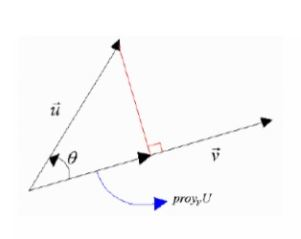
\includegraphics[width=0.5\linewidth]{imagenes/proyeccion} 

}

\caption{Proyección Ortogonal}\label{fig:graf-proy-ortog}
\end{figure}

\begin{definition}[Matriz]
\protect\hypertarget{def:matriz}{}\label{def:matriz}Una matriz es un arreglo rectangular de números en filas y columnas. Usualmente se denotan por \(A_{n \times p}\)
\end{definition}

\begin{definition}[Matriz Cuadrada]
\protect\hypertarget{def:matriz-cuad}{}\label{def:matriz-cuad}\(A_{n \times p}\) es cuadrada si \(n=p\), ie. número de filas igual al número de columnas, se denota por: \(A_n\)
\end{definition}

\begin{definition}[Matriz Diagonal]
\protect\hypertarget{def:matriz-diag}{}\label{def:matriz-diag}Es una matriz cuadrada con ceros fuera de la diagonal, se denota por \(D_n\)
\end{definition}

\begin{definition}[Matriz Identidad]
\protect\hypertarget{def:matriz-ident}{}\label{def:matriz-ident}Es una matriz diagonal con unos en la diagonal, se denota por \(I_n\)
\end{definition}

\begin{definition}[Matriz Cuadrada de unos]
\protect\hypertarget{def:matriz-unos}{}\label{def:matriz-unos}Es una matriz cuadrada llena de unos, se denota por: \(J_n\)
\end{definition}

\begin{definition}[Matriz triangular inferior y triangular superior]
\protect\hypertarget{def:matriz-trinagular}{}\label{def:matriz-trinagular}Matrices con parte superior llena de ceros y parte inferior llena de ceros, respectivamente.
\end{definition}

\begin{definition}[Suma de Matrices]
\protect\hypertarget{def:suma-matrices}{}\label{def:suma-matrices}La suma de matrices de igual dimensión se realiza componente a componente.
\end{definition}

\begin{definition}[Multiplicación de Matrices]
\protect\hypertarget{def:multip-matrices}{}\label{def:multip-matrices}La multiplicación de matrices de dimensiones apropiadas se realiza siguiendo el procedimiento de filas por columnas.
\end{definition}

\begin{definition}[Matriz Traspuesta]
\protect\hypertarget{def:matriz-traspuesta}{}\label{def:matriz-traspuesta}La transpuesta de una matriz \(A_{n \times p}\) es la matriz que se obtiene invirtiendo las filas por columnas, la cual se denota por: \(A_{p \times n}^t\).~~ Se cumple que: \((AB)^t=B^tA^t\).
\end{definition}

\begin{definition}[Matriz Simétrica]
\protect\hypertarget{def:matriz-simetrica}{}\label{def:matriz-simetrica}Una matriz simétrica es una matriz cuadrada \(A_n\) tal que su transpuesta es igual a la matriz original, ie. si \(A^t=A\).
\end{definition}

\begin{definition}[Determinante de una Matriz]
\protect\hypertarget{def:determ-matriz}{}\label{def:determ-matriz}Sea \(A\) una matriz cuadrada de orden \(n\). El determinante de \(A\), denotado por \(|A|\), se obtiene como:
\[
|A|=\sum_{j=1}^n a_{ij}|A_{ij}|(-1)^{i+j},
\]
en donde, \(A_{ij}\)-es la matriz cuadrada de orden \((n-1)\) que se obtiene al eliminar la fila \(i\) y la columna \(j\) de \(A\) (ie. menor \(A_{ij}\)).
\end{definition}

\textbf{Alguna propiedades del determinante de una matriz:}

Sean \(A\) y \(B\) matrices cuadradas de orden \(n\) y \(c\in \mathbb{R}\), entonces:

\begin{enumerate}
\def\labelenumi{\alph{enumi}.}
\item
  \(|A|=|A^t|\)
\item
  \(|AB|=|A||B|\)
\item
  \(|c A|=c^n|A|\)
\item
  La matriz \(A\) es invertible si el \(|A|\neq 0\), esto equivale a decir que todos los valores propios de \(A\) son diferentes de cero.
\item
  Si la inversa de \(A\), \(A^{-1}\)-existe, entonces: \(|A| =\frac{1}{|A^{-1}|}\)
\item
  Si \(A\) es una matriz cuadrada de orden \(2\)-invertible, entonces:
\end{enumerate}

\[
A^{-1}=\frac{1}{|A|}\begin{bmatrix}
                a_{22} & -a_{12}\\
                -a_{21} & a_{11}
                \end{bmatrix}\ , \ \ \ \text{con}\ \ \ A=\begin{bmatrix}
                a_{11} & a_{12}\\
                a_{21} & a_{22}
                \end{bmatrix}
\]

\begin{definition}[Matriz Inversa]
\protect\hypertarget{def:matriz-inversa}{}\label{def:matriz-inversa}Sea \(A_n\) una matriz cuadrada de orden \(n\). Si existe una matriz cuadrada \(B_n\) tal que \(A_n B_n=B_nA_n=I_n\), entonces se dice que \(B\) es la inversa de \(A\) y se denota por: \(B=A^{-1}\), ie.
\[
AA^{-1}=A^{-1}A=I_n
\]
\end{definition}

\textbf{Propiedades de la Inversa:}

La inversa de \(A\), ei. \(A^{-1}\) cumple que:

\begin{enumerate}
\def\labelenumi{\alph{enumi}.}
\item
  \((A^t)^{-1}=(A^{-1})^t\).
\item
  \((AB)^{-1}=B^{-1}A^{-1}\).
\item
  \((A^{-1})^{-1}=A\).
\end{enumerate}

\begin{definition}[Matriz Ortogonal]
\protect\hypertarget{def:matriz-ortog}{}\label{def:matriz-ortog}Una matriz cuadrada \(A_n\) de orden \(n\), se dice que es ortogonal si sus columnas como vectores son perpendiculares, ie:
\[
A^tA=AA^t=I_n,
\]
es decir, si \(A^t=A^{-1}\). (Ortonormal si además son unitarios ).
\end{definition}

\textbf{Propiedades de una matriz Ortogonal:}

\begin{enumerate}
\def\labelenumi{\alph{enumi}.}
\item
  \(|A|=\pm 1\).
\item
  El producto de un número finito de matrices ortogonales es ortogonal.
\item
  La Inversa y por tanto la transpuesta de una matriz ortogonal es ortogonal.
\item
  Dada una matriz \(A\) y una matriz \textit{ortogonal} \(P\), entonces:
  \[
  |A|=|P^tAP|
  \]
\end{enumerate}

\begin{definition}[Vectores Linealmente-Independientes (LI)]
\protect\hypertarget{def:vectores-li}{}\label{def:vectores-li}Un conjunto de \(k\)-vectores, \(\underline{\mathbf{x}}_1,\underline{\mathbf{x}}_2,\ldots,\underline{\mathbf{x}}_k\), se dice que son LI si la ecuación:
\[
c_1\underline{\mathbf{x}}_1+c_2\underline{\mathbf{x}}_2+\ldots+c_k\underline{\mathbf{x}}_k=0,
\]
tiene como única solución la dada por: \(c_1=c_2=\ldots=c_k=0\), para \(c_i \in \mathbb{R}\), \(i=1,2,\ldots,k\)
\end{definition}

\begin{definition}[Valores y Vectores propios de una Matriz]
\protect\hypertarget{def:val-vect-propios}{}\label{def:val-vect-propios}Sea \(A\) una matriz cuadrada de orden \(n\). Se dice que \(\lambda\) es un valor propio de \(A\), asociado al vector propio \(\underline{\mathbf{x}}\), si se cumple que: \(A\underline{\mathbf{x}}=\lambda \underline{\mathbf{x}}\)

Para hallar los valores propios de una matriz \(A\) se resuelve la siguiente ecuación característica: \(|A-\lambda I|=0\).

Al dividir el vector propio \(\underline{\mathbf{x}}\) por su norma \(\|\underline{\mathbf{x}}\|\), se obtiene un vector unitario, el cual se denotará por: \(\underline{e}=\frac{\underline{\mathbf{x}}}{\|\underline{\mathbf{x}}\|}=\frac{\underline{\mathbf{x}}}{\sqrt{\langle \underline{\mathbf{x}}\ , \ \underline{\mathbf{x}} \rangle}}\)
\end{definition}

\textbf{Alguna propiedades sobre los valores propios de una matriz:}

Sean \(A\) y \(B\) matrices cuadradas de orden \(n\) y \(c\in \mathbb{R}\), entonces:

\begin{enumerate}
\def\labelenumi{\alph{enumi}.}
\item
  Una matriz \(A\) tiene al menos un valor-propio igual a cero sii \(A\) es singular (no tiene inversa), ie. sii el \(|A|=0\).
\item
  Si \(A\) es una matriz simétrica con valores propios reales, entonces los vectores propios asociados a valores propios diferentes son ortogonales.
\item
  \textbf{Teorema de Descomposición Espectral:}
\end{enumerate}

Cualquier matriz simétrica \(A\), se puede escribir como:
\[
A=P\mathbf{\Lambda} P^t=P^t\mathbf{\Lambda} P
\]
en donde: \(\mathbf{\Lambda}\)-es una matriz diagonal formada por los valores propios de \(A\), y \(P\)-es una matriz ortogonal cuyas columnas son los vectores propios unitarios asociados a los elementos de la diagonal de \(\mathbf{\Lambda}\), ie.
\[
PP^t=P^tP=I_n.
\]

\begin{enumerate}
\def\labelenumi{\alph{enumi}.}
\setcounter{enumi}{3}
\item
  Si \(A\) es una matriz simétrica, entonces el rango de \(A\), \(r(A)\), es igual al número de sus valores propios no nulos.
\item
  Si \(\lambda_1,\lambda_2,\ldots, \lambda_n\), son los valores propios de \(A\), entonces:
  \[
                 tr(A)=\sum_{i=1}^n \lambda_i\ , \ \ \ \text{y} \ \ \
               |A|=\prod_{i=1}^n \lambda_i
  \]
\item
  Si \(\lambda\) es una valor propio de \(A\), entonces \(\lambda^k\) es un valor propio de \(A^k\).
\item
  Las matrices \(A\) y \(A^t\) tienen el mismo conjunto de valores propios, pero un vector propio de \(A\) no-necesariamente es un vector propio de \(A^t\).
\item
  Si \(A\) es idempotente, entonces sus valores propios son cero o uno.
\end{enumerate}

\begin{definition}[Traza de una Matriz]
\protect\hypertarget{def:traza-matriz}{}\label{def:traza-matriz}La traza de una matriz cuadrada \(A\) de orden \(n\), se define como la suma de los elementos de su diagonal, ie.
\[
tr(A)=\sum_{i=1}^n a_{ii}.
\]
\end{definition}

\textbf{Alguna propiedades de la traza de una matriz:}

Sean \(A\) y \(B\) matrices cuadradas de orden \(n\) y \(c\in \mathbb{R}\), entonces:

\begin{enumerate}
\def\labelenumi{\alph{enumi}.}
\item
  \(tr(c A)=c\ tr(A)\).
\item
  \(tr(A \pm B)=tr(A)\pm tr(B)\).
\item
  \(tr(AB)=tr(BA)\).
\item
  \(tr(A^t)= tr(A)\).
\item
  Si \(B^{-1}\)-existe, entonces: \(tr(B^{-1}AB)=tr(A)\).
\item
  \(tr(ABC)=tr(CAB)=tr(BCA)\).
\item
  \(tr(AA^t)=\sum_{i=1}^n\sum_{j=1}^n a_{ij}^2\).
\end{enumerate}

\begin{definition}[Descomposición Espectral de una Matriz]
\protect\hypertarget{def:descomp-espectral}{}\label{def:descomp-espectral}Sea \(A\) una matriz simétrica de orden \(n\), entonces:
\[
                  A=\lambda_1\underline{e}_1\underline{e}_1^t+
                  \lambda_2\underline{e}_2\underline{e}_2^t+\ldots+
                  \lambda_n\underline{e}_n\underline{e}_n^t=\sum_{i=1}^n \lambda_i\underline{e}_i\underline{e}_i^t
\]
en donde, los \(\underline{e}_i\)-son los vectores propios normalizados de \(A\)-asociados a los valores propios \(\lambda_i\), \(i=1,2,\ldots,n\).

A la descomposición anterior de \(A\)-se le llama descomposición espectral de \(A\).
\end{definition}

\begin{definition}[Matriz Definida y Semi-Definida Positiva]
\protect\hypertarget{def:matriz-def-pos}{}\label{def:matriz-def-pos}Sea \(A\) una matriz simétrica de orden \(n\). Se deice que \(A\) es semi-definida positiva si para todo vector \(\underline{\mathbf{x}}\in \mathbf{R}^n\) distinto del vector nulo se cumple que:
\[
                  \underline{\mathbf{x}}^t A \underline{\mathbf{x}} \geq 0
\]
Se dice que \(A\) es Definida positiva si para todo vector \(\underline{\mathbf{x}}\in \mathbb{R}^n\) distinto del vector nulo se cumple que: \(\underline{\mathbf{x}}^t A\underline{\mathbf{x}} > 0\)
\end{definition}

\textbf{Propiedades de una Matriz Definida Positiva:}

\begin{enumerate}
\def\labelenumi{\alph{enumi}.}
\item
  Si \(A\) es una matriz DP, entonces todos sus valores propios son positivos, lo que equivale a decir que su determinante es distinto de cero y por lo tanto dicha matriz tiene inversa.
\item
  Sea \(A\) una matriz DP. Como \(A\)-es invertible y se tiene que por la descomposición espectral:
  \[
                 A=P\mathbf{\Lambda} P^t=\sum_{i=1}^{n}\lambda_i\underline{e}_i\underline{e}_i^t,\ \ \ \text{entonces:}
  \]
  \[
  A^{-1}=P \mathbf{\Lambda}^{-1}P^t=\sum_{i=1}^{n}\frac{1}{\lambda_i}\underline{e}_i\underline{e}_i^t
  \]
\end{enumerate}

\begin{definition}[Matriz Raíz-Cuadrada]
\protect\hypertarget{def:matriz-raiz-cuadrada}{}\label{def:matriz-raiz-cuadrada}La raíz-cuadrada de \(A\) es:
\[
A^{1/2}=P \mathbf{\mathbf{\mathbf{\mathbf{\mathbf{\Lambda}}}}}^{1/2}P^t=\sum_{i=1}^{n}\sqrt{\lambda_i}\underline{e}_i\underline{e}_i^t
\]
\end{definition}

\textbf{Propiedades de la Matriz Raíz-Cuadrada:}

La matriz raíz-cuadrada dada por:
\[
A^{1/2}=P \mathbf{\mathbf{\mathbf{\mathbf{\mathbf{\Lambda}}}}}^{1/2}P^t=\sum_{i=1}^{n}\sqrt{\lambda_i}\underline{e}_i\underline{e}_i^t
\]
tiene las siguientes propiedades:

\begin{enumerate}
\def\labelenumi{\alph{enumi}.}
\item
  \[
  (A^{1/2})^{'}=A^{1/2}, \ \ \ \ \text{es decir:} \ \ A^{1/2}-\text{es simétrica.}
  \]
\item
  \[
  A^{1/2}A^{1/2}=A.
  \]
\item
  \[
  (A^{1/2})^{-1}=P\mathbf{\mathbf{\mathbf{\mathbf{\mathbf{\Lambda}}}}}^{-1/2}P^t=\sum_{i=1}^{n}\frac{1}{\sqrt{\lambda_i}}\underline{e}_i\underline{e}_i^t
  \]
\item
  \[
  A^{1/2}A^{-1/2}=A^{-1/2}A^{1/2}=I,\ \ \ \text{y} \ \ \ A^{-1/2}A^{-1/2}=A^{-1},
  \]
  donde \(A^{-1/2}=(A^{1/2})^{-1}\)
\end{enumerate}

\textbf{Además:}

\[
\mathbf{\Lambda}^{-1/2}-\text{Matriz diagonal con:}\ \ \  1/\sqrt{\lambda_i} \ \ \ \text{en la diagonal}.
\]

\[
\mathbf{\Lambda}^{1/2}-\text{Matriz diagonal con:}\ \ \  \sqrt{\lambda_i}\ \ \ \text{en la diagonal}.
\]

\[
\mathbf{\Lambda}^{-1}-\text{Matriz diagonal con:}\ \ \  1/\mathbf{\lambda_i}\ \ \ \text{en la diagonal}.
\]

\begin{definition}[Forma Cuadrática]
\protect\hypertarget{def:forma-cuadratica}{}\label{def:forma-cuadratica}Sea \(A_p\) una matriz simétrica de orden \(p\) y \(\underline{\mathbf{x}}\) un vector \(p\times 1\), entonces a las función:
\[
Q(\underline{\mathbf{x}})=\underline{\mathbf{x}}^t A \underline{\mathbf{x}}
\]
se le llama forma cuadrática de \(\underline{\mathbf{x}}\).

\(Q(\underline{\mathbf{x}})\)-es un escalar y puede expresarse alternativamente por la ecuación:
\[
Q(\underline{\mathbf{x}})=\sum_{i=1}^p \sum_{j=1}^p a_{ij}x_i x_j,
\]
con \(a_{ij}\)-elementos de la matriz \(A\) y \(x_i\), \(x_j\) elementos del vector \(\underline{\mathbf{x}}\).

Si \(Q(\underline{\mathbf{x}})\geq 0\), \(\forall \underline{\mathbf{x}} \neq \underline{\mathbf{0}}\), entonces \(A\)-se llama semi-definida positiva y se escribe \(A\geq 0\) y si \(Q(\underline{\mathbf{x}})> 0\), \(\forall \underline{\mathbf{x}} \neq \underline{\mathbf{0}}\), entonces \(A\)-se llama definida positiva y se escribe \(A> 0\).
\end{definition}

\textbf{Algunas Propiedades de Formas-Cuadráticas:}

\begin{enumerate}
\def\labelenumi{\alph{enumi}.}
\item
  Si \(A>0\) entonces, todos sus valores propios son positivos.
\item
  Si \(A \geq 0\) entonces, \(\lambda_i \geq 0\) para \(i=1,2,\ldots,p\) y \(\lambda_i=0\) para algún \(i\).
\item
  Si \(A > 0\) entonces, \(A\)-es no-singular y en consecuencia \(|A|>0\).
\item
  Si \(A>0\) entonces, \(A^{-1}>0\).
\item
  Si \(A>0\) y \(C_p\)-es una matriz no-singular entonces, \(C^tAC>0\).
\item
  Sea \(A\) es una matriz simétrica de orden \(p\) y sea \(\underline{\mathbf{x}}\)-un vector, entonces:
  \[
  \underline{\mathbf{x}}^t A \underline{\mathbf{x}}=t(\underline{\mathbf{x}}^t A \underline{\mathbf{x}})=t( A \underline{\mathbf{x}}\underline{\mathbf{x}}^t)
  \]
\end{enumerate}

\hypertarget{diferenc_vectores}{%
\section{Diferenciación con Vectores y Matrices}\label{diferenc_vectores}}

\begin{definition}[Función Vectorial]
\protect\hypertarget{def:funcion-vectorial}{}\label{def:funcion-vectorial}Sea \(f\)-una función que asigna a un vector \(\underline{x}\in \mathbb{R}^p\) un número real, ie.
\begin{align*}
f \ \ \ \ &: \ \ \ \ \mathbb{R}^p \ \ \ \longrightarrow \ \ \ \mathbb{R}\\
& \hspace{-1cm} \underline{x}=(x_1,x_2,\ldots,x_p) \longrightarrow f(\underline{x}).
\end{align*}
La derivada de \(f(\underline{x})\) con respecto a \(\underline{x}\) se define como el vector dado por:
\[
\frac{\partial f(\underline{x})}{\partial \underline{x}}=\begin{bmatrix}
\frac{\partial f(\underline{x})}{\partial \underline{x}_1} \\
\frac{\partial f(\underline{x})}{\partial \underline{x}_2}\\
\vdots \\
\frac{\partial f(\underline{x})}{\partial \underline{x}_p}
\end{bmatrix}\in \mathbb{R}^p.
\]
Al vector anterior se le llama: \emph{Vector-Gradiente}.
\end{definition}

\hypertarget{vector-gradiente-para-diferentes-definiciones-de-funderlinex}{%
\subsection{\texorpdfstring{Vector-Gradiente para diferentes definiciones de \(f(\underline{x})\):}{Vector-Gradiente para diferentes definiciones de f(\textbackslash underline\{x\}):}}\label{vector-gradiente-para-diferentes-definiciones-de-funderlinex}}

\begin{enumerate}
\def\labelenumi{\arabic{enumi}.}
\item
  Si \(f(\underline{x})=\underline{a}^t\underline{x}=\underline{x}^t\underline{a}\), entonces:
  \[
  \frac{\partial f(\underline{x})}{\partial \underline{x}}=\frac{\partial (\underline{a}^t\underline{x})}{\partial \underline{x}}=\frac{\partial (\underline{x}^t\underline{a})}{\partial \underline{x}}= \begin{bmatrix}
  \frac{\partial f}{\partial x_1} \\\frac{\partial f}{\partial x_2} \\ \vdots \\ \frac{\partial f}{\partial x_p}
  \end{bmatrix}   =  \begin{bmatrix}
  a_1 \\ a_2\\ \vdots \\ a_p
  \end{bmatrix} =\underline{a}.
  \]
\item
  Si \(f(\underline{x})=\underline{x}^t A\) (vector fila), con \(A_{p\times p}\)- entonces:
  \[
  \frac{\partial f(\underline{x})}{\partial \underline{x}}=\frac{\partial (\underline{x}^t A)}{\partial \underline{x}}= A, \ \ \ \text{A-como columnas}.
  \]
  Si \(f(\underline{x})=A^t\underline{x}\) (vector columna), con \(A_{p\times p}\)- entonces:
  \[
  \frac{\partial f(\underline{x})}{\partial \underline{x}}=\frac{\partial (A^t\underline{x})}{\partial \underline{x}}= A, \ \ \ \text{A-como filas}.
  \]
\item
  Derivada de una forma-cuadrática:
\end{enumerate}

Si \(f(\underline{x})=\underline{x}^t A \underline{x}\), con \(A_{p\times p}\)-matriz entonces:

a.) \(\frac{\partial f(\underline{x})}{\partial \underline{x}}=\frac{\partial (\underline{x}^t A \underline{x})}{\partial \underline{x}}=A^t\underline{x}+A\underline{x}\).

b.) Si \(A\)- es simétrica entonces: \(\frac{\partial f(\underline{x})}{\partial \underline{x}}=\frac{\partial (\underline{x}^t A \underline{x})}{\partial \underline{x}}=2A\underline{x}\).

\begin{enumerate}
\def\labelenumi{\arabic{enumi}.}
\setcounter{enumi}{3}
\tightlist
\item
  Derivada de la Inversa de una Matriz: \(f(\mathbf{X})=\mathbf{X}^{-1}\)
\end{enumerate}

La derivada de la inversa de una matriz no-singular \(\mathbf{X}_{p\times p}\) respecto a su elemento en la posición \(ij\), ie. respecto a \(x_{ij}\) es:

a.) \(\frac{\partial f(\mathbf{X})}{\partial x_{ij}}=\frac{\partial (\mathbf{X}^{-1})}{\partial x_{ij}}=-\mathbf{X}^{-1}.\frac{\partial \mathbf{X}}{\partial x_{ij}}. \mathbf{X}^{-1}=-\mathbf{X}^{-1}.\Delta_{ij}. \mathbf{X}^{-1}\), si todos los elemntos de \(\mathbf{X}\)-son diferentes.

b.) Si \(\mathbf{X}\)-es simétrica entonces:

\(\frac{\partial f(\mathbf{X})}{\partial x_{ij}}=\frac{\partial (\mathbf{X}^{-1})}{\partial x_{ij}}=-\mathbf{X}^{-1}.(\Delta_{ij}+\Delta_{ji}). \mathbf{X}^{-1}\), si \(i\neq j\).

\(\frac{\partial f(\mathbf{X})}{\partial x_{ij}}=\frac{\partial (\mathbf{X}^{-1})}{\partial x_{ij}}=-\mathbf{X}^{-1}.\Delta_{ii}. \mathbf{X}^{-1}\), si \(i= j\).

Donde, \(\Delta_{ij}=\frac{\partial (\mathbf{X})}{\partial x_{ij}}\)-es una matriz tal que en el lugar donde se ubica el elemento \(x_{ij}\)-tiene un uno y en los demás lugares tiene ceros.

\begin{enumerate}
\def\labelenumi{\arabic{enumi}.}
\setcounter{enumi}{4}
\tightlist
\item
  Derivada del Determinante de una Matriz: \(f(\mathbf{X})=|\mathbf{X}|\)\\
\end{enumerate}

La derivada del determinante de una matriz no-singular \(\mathbf{X}_{p\times p}\) respecto a su elemento en la posición \(ij\), ie. respecto a \(x_{ij}\) es:

\begin{itemize}
\item
  \(\frac{\partial f(\mathbf{X})}{\partial x_{ij}}=\frac{\partial |\mathbf{X}|}{\partial x_{ij}}=\mathbf{X}_{ij}\), en donde: \(\mathbf{X}_{ij}\)-es el cofactor de \(x_{ij}\).
\item
  La matriz de derivadas es: \(\frac{\partial |\mathbf{X}|}{\partial \mathbf{X}}=(\mathbf{X}_{ij})\).
\item
  Para matrices simétricas \(\mathbf{X}\), la matriz de derivadas es:
  \[
  \frac{\partial |\mathbf{X}|}{\partial \mathbf{X}}=2 \text{adj}(\mathbf{X})-\text{Diag}[\text{adj}(\mathbf{X})]=|\mathbf{X}
  |[2\mathbf{X}^{-1}-\text{Diag}(\mathbf{X}^{-1})].
  \]
  donde, \(\text{Diag}[\text{adj}(\mathbf{X})\)-es la matriz diagonal de la adjunta de \(\mathbf{X}\).
\end{itemize}

La adjunta de \(\mathbf{X}\), adj\((\mathbf{X})\)-es la transpuesta de la matriz de cofactores de \(\mathbf{X}\).

La matriz de cofactores de \(\mathbf{X}\), se obtiene al reemplazar los elementos \(x_{ij}\) de \(\mathbf{X}\) por los respectivos cofactores.

El cofactor \(C_{ij}=\mathbf{X}_{ij}\) de \(\mathbf{X}\) se define como:
\[
C_{iji}=(-1)^{i+j}|X_{ij}|,
\]
donde, \(X_{ij}\)- es el menor del elemento \(x_{ij}\), ie. matriz obtenida al borrar la fila \(i\) y la columna \(j\) de \(\mathbf{X}\).

\begin{enumerate}
\def\labelenumi{\arabic{enumi}.}
\setcounter{enumi}{5}
\tightlist
\item
  Derivada de la traza de una Matriz: \(f(\mathbf{X})=tr(\mathbf{X})\)
\end{enumerate}

La derivada de la traza de una matriz \(\mathbf{X}_{p\times p}\) es:
\[
\frac{\partial f(\mathbf{X})}{\partial \mathbf{X}}=\frac{\partial [tr(\mathbf{X})] }{\partial \mathbf{X}}=I_p,
\]
de donde:

\begin{itemize}
\item
  \(\frac{\partial [tr(\mathbf{X}A)] }{\partial \mathbf{X}}=A^{'}\),~~ si \(\mathbf{X}\)-es no-simétrica.
\item
  \(\frac{\partial [tr(\mathbf{X}A)] }{\partial \mathbf{X}}=A+A^{'}-\text{Diag}(A)\),~~si \(\mathbf{X}\)-es simétrica.
\end{itemize}

\begin{enumerate}
\def\labelenumi{\arabic{enumi}.}
\setcounter{enumi}{6}
\tightlist
\item
  Derivada del logaritmo del determinante de una matriz:
\end{enumerate}

\(f(\mathbf{X})=\text{Log}(|\mathbf{X}|)\)

La derivada del logaritmo del determinante de una matriz \(\mathbf{X}_{p\times p}\) es:
\[
\frac{\partial f(\mathbf{X})}{\partial \mathbf{X}}=\frac{\partial \text{Log}(|\mathbf{X}|)}{\partial \mathbf{X}}=\frac{1}{|\mathbf{X}|}\frac{\partial |\mathbf{X}|}{\partial \mathbf{X}}=2\mathbf{X}^{-1}-\text{Diag}(\mathbf{X}^{-1}).
\]

\begin{theorem}[Teorema de Maximización]
\protect\hypertarget{thm:teorema-maximo}{}\label{thm:teorema-maximo}Dada una matríz simétrica definida positiva \(\mathbf{B}_{p\times p}\) y un \(b>0\), entonces:
\[
\frac{1}{|\mathbf{\mathbf{\Sigma}}|^{b}}
  e^{-\frac{1}{2} \text{tr}\left(   \mathbf{\mathbf{\Sigma}}^{-1} \mathbf{B} \right)} \leq
\frac{1}{|\mathbf{B}|^{b}} (2b)^{(pb)}
  e^{-bp} \ , \ \ \ \forall \ \ \text{matriz} \ \ \mathbf{\mathbf{\Sigma}} \ \ \text{Def +},
\]
y la igualdad se cumple sólo cuando:
\(\mathbf{\mathbf{\Sigma}}=\left(\frac{1}{2b} \right)\mathbf{B}\).
\end{theorem}

\hypertarget{org_pres_dat}{%
\section{Organización y Presentación de Datos}\label{org_pres_dat}}

\hypertarget{resumenes-descriptivos}{%
\subsection{Resumenes Descriptivos}\label{resumenes-descriptivos}}

\textbf{Matriz de Datos}

La matriz de datos muestrales se representa por:
\[
\mathbf{X}_{n\times p}=\begin{bmatrix}
x_{11} & x_{12} & \cdots & x_{1p}\\
x_{21} & x_{22} & \cdots & x_{2p}\\
\vdots & \vdots & & \vdots \\
x_{n1} & x_{n2} & \cdots & x_{np}
\end{bmatrix}=
\begin{bmatrix}
\underline{\mathbf{x}}_1 \\ \underline{\mathbf{x}}_2 \\ \vdots \\ \underline{\mathbf{x}}_n
\end{bmatrix}=
\begin{bmatrix}
\underline{\mathbf{x}}^{(1)} & \underline{\mathbf{x}}^{(2)} & \cdots & \underline{\mathbf{x}}^{(n)}
\end{bmatrix}
\]

Se tienen \(n\)-vectores \(\underline{\mathbf{x}}_i\) para \(i=1,2,\cdots,n\) en \(\mathbb{R}^p\) con media dada por: \(E[\underline{\mathbf{x}}_i]=
{\large \underline{\mathbf{\mu}}}\ _{p\times 1}\) y matriz de var-cov dada por: \(Cov[\underline{\mathbf{x}}_i]=\mathbf{\Sigma}_{p\times p}\).

\textbf{Estadísticos descriptivos}

Debido a la necesidad de hacer inferencias acerca de los parámetros poblacionales de una cierta distribución poblacional multivariada, es necesario definir algunos \emph{Estadísticos Descriptivos}.

En el caso multivariado los parámetros poblacionales de interés son el vector de medias poblacional \(
{\large \underline{\mathbf{\mu}}}\ \), combinaciones lineales del vector de medias poblacional y la matriz de var-cov poblacional \(\mathbf{\mathbf{\Sigma}}\).

Los respectivos estadísticos descriptivos asociados a estos parámetros poblacionales son el vector de medias muestrales \(\underline{\overline{\mathbf{x}}}\), combinaciones lineales de dicho vector y la matriz de var-cov muestrales \(\mathbf{S}\) o \(\mathbf{S}_n\).

\textbf{Algunas Notaciones}

En la definción del vector de medias muestrales y matriz de var-cov muestrales, se deben de tener en cuenta las siguientes notaciones.

En el vector de medias muestrales,
\[
\underline{\overline{\mathbf{x}}}_{p\times 1} =\begin{bmatrix}
\bar{X}_1 \\ \bar{X}_2 \\ \vdots \\ \bar{X}_p
\end{bmatrix}
\]
se tiene que:
\[
\overline{X}_{k}=\frac{1}{n}\sum_{j=1}^n x_{jk}
\]
para \(k=1,2,\cdots, p\).

En la matrix de Var-Cov muestrales:
\[
\mathbf{S}=\begin{bmatrix}
s_{11} & s_{12} & \cdots & s_{1p}\\
s_{21} & s_{22} & \cdots & s_{2p}\\
\vdots & \vdots & \ddots & \vdots\\
s_{p1} & s_{p2} & \cdots & s_{pp}\\
\end{bmatrix}=\frac{1}{n-1}\sum_{k=1}^n(\underline{\mathbf{x}}_k - \underline{\overline{\mathbf{x}}})(\underline{\mathbf{x}}_k - \underline{\overline{\mathbf{x}}})^T ,
\]
se tiene que:
\[
s_{kk}=\frac{1}{n-1}\sum_{j=1}^n (x_{jk}-\overline{x}_k)^2, \ \ k=1,2,\cdots,p, \ \ \ \text{y}
\]
\[
s_{ik}=\frac{1}{n-1}\sum_{j=1}^n (x_{ji}-\overline{x}_i)(x_{jk}-\overline{x}_k), \ \ i,k=1,2,\cdots,p,
\]
que representan la varianza muestral de \(X^{(k)}\) y la covarianza muestral entre \(X^{(i)}\) y \(X^{(k)}\), para \(i,k=1,2,\cdots,p\).

En la matrix de Correlaciones-muestrales:
\[
\mathbf{R}=\begin{bmatrix}
1 & \gamma_{12} & \cdots & \gamma_{1p} \\
\gamma_{21} & 1 & \cdots & \gamma_{2p} \\
\vdots & \vdots & \ddots & \vdots \\
\gamma_{p1} & \gamma_{p2} & \cdots & \gamma_{pp} \\
\end{bmatrix} ,
\]
se tiene que:
\[
\gamma_{ik}=\frac{s_{ik}}{\sqrt{s_{ii}}\sqrt{s_{kk}}}, \ \ i,k=1,2,\cdots,p,
\]
que representan la correlación muestral entre \(X^{(i)}\) y \(X^{(k)}\), para \(i,k=1,2,\cdots,p\).

\(\gamma_{ik}\)-no depende de las unidades de medida.

\(\gamma_{ik}=\gamma_{ki}\).

\(-1\leq \gamma_{ik}\leq 1\).

\(\gamma_{ik}\)-es la covarianza muestral de las observaciones estandarizadas.

\hypertarget{representaciuxf3n-gruxe1fica-de-observaciones-multivariadas}{%
\subsection{Representación Gráfica de Observaciones multivariadas}\label{representaciuxf3n-gruxe1fica-de-observaciones-multivariadas}}

\textbf{Algunas gráficas importantes son:}

\begin{itemize}
\tightlist
\item
  Histogramas
\item
  Diagramas de barras
\item
  Bix-Plot
\item
  Gráficos de dispersión y matriz de dispersión
\item
  Gráficos tridimensionales y de contornos
\item
  Gráficos de estrellas
\item
  Gráfico de caras de Chernoff
\item
  Gráficos de normales bivariadas
\item
  Gráficos de Cluster
\end{itemize}

\hypertarget{vectores-y-matrices-aleatorias}{%
\subsection{Vectores y Matrices Aleatorias}\label{vectores-y-matrices-aleatorias}}

\begin{definition}[Vector Aleatorio]
\protect\hypertarget{def:vector-aleatorio}{}\label{def:vector-aleatorio}Un vector aleatorio es aquel cuyas componentes son variables aleatorias.
\end{definition}

\begin{definition}[Matriz Aleatoria]
\protect\hypertarget{def:matriz-aleatoria}{}\label{def:matriz-aleatoria}Una matriz aleatoria es aquella cuyas componentes son variables aleatorias.
\end{definition}

\begin{definition}[Valor esperado de una matriz (o vector) Aleatoria]
\protect\hypertarget{def:valor-espera-mat}{}\label{def:valor-espera-mat}El valor esperado de una matriz aleatoria (o de un vector aleatorio) es una matriz ( o un vector) cuyos elementos son los valores esperados de cada entrada de la matriz, ie. el valor esperado de cada una de las variables aleatorias consideradas.
\end{definition}

\begin{definition}[Vector de medias poblacional]
\protect\hypertarget{def:vector-medias}{}\label{def:vector-medias}Dado un vector-aleatorio:
\[
\underline{\mathbf{x}}=\begin{bmatrix}
X_1 \\ X_2 \\ \vdots \\ X_p
\end{bmatrix}
\]
el vector de medias está dado por:
\[
\underline{\mu}=E[\underline{\mathbf{x}}]=\begin{bmatrix}
\mu_1\\ \mu_2 \\ \vdots \\  \mu_p
\end{bmatrix}=\begin{bmatrix}
E[X_1]\\ E[X_2]\\ \vdots \\ E[X_p]
\end{bmatrix}
\]
\end{definition}

\begin{definition}[Matriz de Var-Cov poblacional]
\protect\hypertarget{def:matriz-var-cov}{}\label{def:matriz-var-cov}Dado un vector-aleatorio
\[
\underline{\mathbf{x}}=\begin{bmatrix}
X_1\\X_2\\ \vdots \\ X_p
\end{bmatrix}
\]
la matriz de Var-Cov de \(\underline{\mathbf{x}}\) está dado por:
\begin{align*}
\mathbf{\Sigma}&:=E[(\underline{\mathbf{x}}-\mathbf{\underline{\mu}})(\underline{\mathbf{x}}-\mathbf{\underline{\mu}})^{'}]\\
&\hspace{-0.5cm}= \begin{bmatrix}
\sigma_{11} & \sigma_{12}& \cdots &  \sigma_{1p}\\
\sigma_{21} & \sigma_{22}& \cdots &  \sigma_{2p}\\
\vdots & \vdots & \ddots & \vdots\\
\sigma_{p1}& \sigma_{p2}& \cdots &  \sigma_{pp}
\end{bmatrix}=\begin{bmatrix}
Var[X_1]& Cov[X_1,X_2]& \cdots & Cov[X_1,X_p]\\
Cov[X_2,X_1]& Var[X_2]& \cdots & Cov[X_2,X_p]\\
\vdots & \vdots & \ddots & \vdots\\
Cov[X_p,X_1]& Cov[X_p,X_2]& \cdots & Var[X_p]
\end{bmatrix}
\end{align*}
donde,
\[
\sigma_{ij}=E[(X_i-\mu_i)(X_j-\mu_j)]=Cov(X_i,X_j) \ \ \  y \ \ \ \sigma_{ii}=E[(X_i-\mu_i)^2]=Var(X_i)
\]
\end{definition}

\begin{definition}[Media Marginal de Xi]
\protect\hypertarget{def:media-marginal}{}\label{def:media-marginal}\[
\mu_i=E[X_i]=\begin{cases}
\int_{\mathbb{R}}x_{i}f_{i}(x_{i})dx_{i} \ \ ; \ \ \text{para} \ \ X_{i}-\text{contínua}\\ \\
\sum x_{i}p_{i}(x_{i})\ \ ; \ \ \text{para} \ \ X_{i}-\text{discreta}
\end{cases}
\]
A \(\mu_i\)-se le llama la media poblacional marginal de \(X_i\).
\end{definition}

\begin{definition}[Varianza Marginal de Xi]
\protect\hypertarget{def:var-marginal}{}\label{def:var-marginal}\[
\sigma_i^2=Var[X_i]=\begin{cases}
\int_{\mathbb{R}}(x_{i}-\mu_i)^2f_{i}(x_{i})dx_{i} \ \ ; \ \ \text{para} \ \ X_{i}-\text{cont.}\\ \\
\sum (x_{i}-\mu_i)^2p_{i}(x_{i})\ \ ; \ \ \text{para} \ \ X_{i}-\text{discreta}
\end{cases}
\]
A \(\sigma_i^2\)-se le llama la varianza poblacional marginal de \(X_i\).

\(\Rightarrow\) ~~El comportamiento conjunto de cada par de variables
aleatorias \(X_i\) y \(X_k\) está descrito por su función de distribución
\textbf{conjunta}.
\end{definition}

\begin{definition}[La covarianza poblacional]
\protect\hypertarget{def:cov-pob}{}\label{def:cov-pob}Es una medida de la asociación
lineal en la población de las variables \(X_i\) y \(X_k\):
\[
\sigma_{ik}=E[(X_i-\mu_i)(X_k-\mu_k)] \ \ , \ \ \ \text{donde:}
\]
\vspace{-0.5cm} \[
    \hspace{-1.5cm} Cov[X_{i},X_k]=\sigma_{ik}=\begin{cases}
  \int_{\mathbb{R}}\int_{\mathbb{R}} (x_{i}-\mu_i)(x_{k}-\mu_k )f_{ik}(x_{i},x_k)dx_{i}dx_k \ \ \\ \ \ \text{para} \ \ X_{i},X_k-\text{contínuas}\\ \\
  \sum \sum (x_{i}-\mu_i)(x_k-\mu_k)p_{ik}(x_{i},x_k)\ \ \\ \ \ \text{para} \ \ X_{i},X_k-\text{discretas}
  \end{cases}
\]
A \(\sigma_{ik}\)-se le llama la covarianza poblacional de \(X_i\) y \(X_k\).
\end{definition}

\begin{definition}[Matriz de Correlación poblacional]
\protect\hypertarget{def:matriz-cor}{}\label{def:matriz-cor}Dado un vector-aleatorio
\[
\underline{\mathbf{x}}=\begin{bmatrix}
X_1\\X_2\\ \vdots \\ X_p
\end{bmatrix}
\]
la matriz de Correlación de \(\underline{\mathbf{x}}\) está dado por:
\begin{align*}
\rho
= \begin{bmatrix}
1 & \rho_{12}& \cdots &  \rho_{1p}\\
\rho_{21} & 1 & \cdots &  \rho_{2p}\\
\vdots & \vdots & \ddots & \vdots\\
\rho_{p1}& \rho_{p2}& \cdots &  \rho_{pp}
\end{bmatrix}=\begin{bmatrix}
Corr[X_1,X_1]& Corr[X_1,X_2]& \cdots & Corr[X_1,X_p]\\
Corr[X_2,X_1]& Corr[X_2,X_1]& \cdots & Corr[X_2,X_p]\\
\vdots & \vdots & \ddots & \vdots\\
Corr[X_p,X_1]& Corr[X_p,X_2]& \cdots & Corr[X_p,X_p]
\end{bmatrix}
\end{align*}
donde,
\[
\rho_{ij}=\frac{\sigma_{ij}}{\sqrt{\sigma_{ii}}\sqrt{\sigma_{jj}}}=Corr(X_i,X_j)
\]
\end{definition}

\textbf{Relación entre \(\mathbf{\Sigma}\) y \(\mathbf{\rho}\):}

Dada la matriz diagonal:
\[
\mathbf{\mathbf{\mathbf{\mathbf{\mathbf{\mathbf{\Lambda}}}}}}^{1/2}:=
= \begin{bmatrix}
\sqrt{\sigma_{11}} & &  &  \\
& \sqrt{\sigma_{22}} &  &  \\
&  & \ddots & \\
& &  &  \sqrt{\sigma_{pp}}
\end{bmatrix}
\]
se cumple que:
\[
\mathbf{\Sigma}=\mathbf{\mathbf{\mathbf{\mathbf{\mathbf{\Lambda}}}}}^{1/2}\rho \mathbf{\mathbf{\mathbf{\mathbf{\mathbf{\Lambda}}}}}^{1/2}
\]
y
\[
\rho=(\mathbf{\mathbf{\mathbf{\mathbf{\mathbf{\Lambda}}}}}^{1/2})^{-1}\mathbf{\Sigma} (\mathbf{\mathbf{\mathbf{\mathbf{\mathbf{\Lambda}}}}}^{1/2})^{-1}
\]

\begin{example}[Distribución Bi-Variada Discreta]
\protect\hypertarget{exm:distrib-bivar}{}\label{exm:distrib-bivar}Hallar la matriz de var-cov del vector aleatorio bi-dimensional \(\underline{\mathbf{x}}^t=(X_1,X_2)\), cuya función de densidad de probabilidad conjunta está dada por:
\[
\begin{array}{cc|ccc|c}
&  & & X_2 & & \\
&  & 0 && 1 & \color{red}{ P_1(X_1)} \\\hline
& -1 & 0.24 && 0.06 & \color{red}{ 0.3}\\
X_1 & 0 & 0.16 && 0.14 & \color{red}{ 0.3} \\
& 1 & 0.4 && 0.0 & \color{red}{ 0.4} \\\hline
& \color{red}{ P_2(X_2)} & \color{red}{ 0.8} && \color{red}{ 0.2} & \color{blue}{ 1}
\end{array}
\]
Primero se halla: \(\mu_1=E[X_1]=0.1\), ~~\(\mu_2=E[X_2]=0.2\),
\[
\sigma_{11}=E[(X_1-\mu_1)^{2}]=\sum_{x_1} (x_1-\mu_1)^2P_1(x_1)=0.69
\]
y
\[
\sigma_{22}=E[(X_2-\mu_2)^{2}]=\sum_{x_2} (x_2-\mu_2)^2P_2(x_2)=0.16
\]
\[
\sigma_{12}=E[(X_1-\mu_1)(X_2-\mu_2)]=\sum_{x_1,x_2} (x_1-\mu_1)(x_2-\mu_2)P_{12}(x_1,x_2)=-0.08,
\]
luego:
\[
\underline{\mu}=E[\underline{\mathbf{x}}]=\begin{bmatrix}
E[X_1] \\ E[X_2]
\end{bmatrix}=
\begin{bmatrix}
\mu_1 \\ \mu_2
\end{bmatrix}=
  \begin{bmatrix}
0.1 \\ 0.2
\end{bmatrix} \ \ \text{y}
\]
\begin{align*}
\mathbf{\Sigma} &= E[(\underline{\mathbf{x}}-\underline{\mu})(\underline{\mathbf{x}}-\underline{\mu})^t]\\
&=E\begin{bmatrix}
(X_1-\mu_1)^2 & (X_1-\mu_1)(X_2-\mu_2)\\
(X_2-\mu_2)(X_1-\mu_1) & (X_2-\mu_2)^2
\end{bmatrix}\\ \\
&=\begin{bmatrix}
E(X_1-\mu_1)^2 & E(X_1-\mu_1)(X_2-\mu_2)\\
E(X_2-\mu_2)(X_1-\mu_1) & E(X_2-\mu_2)^2
\end{bmatrix}\\ \\
\mathbf{\Sigma} &=\begin{bmatrix}
\sigma_{11} & \sigma_{12}\\
\sigma_{21} & \sigma_{22}
\end{bmatrix}=
\begin{bmatrix}
0.69 & -0.08 \\
-0.08 & 0.16
\end{bmatrix}
\end{align*}
Luego,
\[
\mathbf{\mathbf{\mathbf{\mathbf{\mathbf{\Lambda}}}}}^{1/2}:=
= \begin{bmatrix}
\sqrt{\sigma_{11}} &   \\
& \sqrt{\sigma_{22}}
\end{bmatrix}=\begin{bmatrix}
\sqrt{0.69} & \\
& \sqrt{0.16}
\end{bmatrix}
\]
de donde:
\[
  (\mathbf{\mathbf{\mathbf{\mathbf{\mathbf{\Lambda}}}}}^{1/2})^{-1}:=
  \begin{bmatrix}
\frac{1}{\sqrt{\sigma_{11}}} &   \\
& \frac{1}{\sqrt{\sigma_{22}}}
\end{bmatrix}=\begin{bmatrix}
\frac{1}{\sqrt{0.69}} & \\
& \frac{1}{\sqrt{0.16}}
\end{bmatrix}
\]
\begin{align*}
\text{y por lo tanto:}\ \ \  \rho &=(\mathbf{\mathbf{\mathbf{\mathbf{\mathbf{\Lambda}}}}}^{1/2})^{-1}\Sigma (\mathbf{\mathbf{\mathbf{\mathbf{\mathbf{\Lambda}}}}}^{1/2})^{-1}\\
&=\begin{bmatrix}
\frac{1}{\sqrt{0.69}} & \\
& \frac{1}{\sqrt{0.16}}
\end{bmatrix}\begin{bmatrix}
0.69 & -0.08 \\
-0.08 & 0.16
\end{bmatrix}
\begin{bmatrix}
\frac{1}{\sqrt{\sigma_{11}}} &   \\
& \frac{1}{\sqrt{\sigma_{22}}}
\end{bmatrix}\\
&=\begin{bmatrix}
1 & -0.24\\
-0.24  & 1
\end{bmatrix}\\
\rho&=\begin{bmatrix}
1 & Corr(X_1,X_2)\\
Corr(X_2,X_1) & 1
\end{bmatrix}
\end{align*}
\end{example}

\begin{example}[Distribución Bi-Variada Discreta-2]
\protect\hypertarget{exm:distrib-bivar-2}{}\label{exm:distrib-bivar-2}Suponga que la matriz de Var-Cov del vector-aleatorio tri-dimensional:\newline \(\underline{\mathbf{x}}=(X_1,X_2,X_3)^t\) es:
\[
\mathbf{\Sigma}=\begin{bmatrix}
4 & 1 & 2 \\
1 & 9 & -3 \\
2 & -3 & 25
\end{bmatrix}=
  \begin{bmatrix}
\sigma_{11} & \sigma_{12} & \sigma_{13}\\
\sigma_{21} & \sigma_{22} & \sigma_{23}\\
\sigma_{31} & \sigma_{32} & \sigma_{33}
\end{bmatrix}
\]
Hallar: \(\rho\).
\end{example}

\hypertarget{vectores-y-matrices-poblacionales-particionados}{%
\section{Vectores y Matrices Poblacionales Particionados}\label{vectores-y-matrices-poblacionales-particionados}}

\hypertarget{particionamiento-del-vector-de-medias-poblacionales}{%
\subsection{Particionamiento del Vector de Medias-Poblacionales}\label{particionamiento-del-vector-de-medias-poblacionales}}

Sea \(\underline{\mathbf{x}}\)-un vector-aleatorio \(p\)-dimensional, entonces se tienen los siguientes particionamientos para el vector de variables aleatoria \(\underline{\mathbf{x}}\), el vector de medias poblacionales \(\underline{\mathbf{\mu}}\) y la matriz de var-cov poblacionales \(\mathbf{\Sigma}\), dadas por:
\[
\underline{\mathbf{x}}=\begin{bmatrix}
X_1 \\ X_2 \\  \vdots  \\ X_p
\end{bmatrix}=\begin{bmatrix}
X_1 \\ \vdots \\ X_q \\ \cdots \\ X_{q+1} \\ \vdots  \\ X_p
\end{bmatrix} =\begin{bmatrix}
\underline{\mathbf{x}}^{(1)} \\ \cdots \\ \underline{\mathbf{x}}^{(2)}
\end{bmatrix} \ \ \ \text{y} \ \ \
\underline{\mu}=E[\underline{\mathbf{x}}]=\begin{bmatrix}
\mu_1 \\ \vdots \\ \mu_q \\ \cdots \\ \mu_{q+1} \\ \vdots  \\ \mu_p
\end{bmatrix} =\begin{bmatrix}
\underline{\mu}^{(1)} \\ \cdots \\ \underline{\mu}^{(2)}
\end{bmatrix}
\]

\hypertarget{particionamiento-de-la-matriz-de-var-cov-poblacional-mathbfsigma}{%
\subsection{\texorpdfstring{Particionamiento de la Matriz de Var-Cov Poblacional \(\mathbf{\Sigma}\)}{Particionamiento de la Matriz de Var-Cov Poblacional \textbackslash mathbf\{\textbackslash Sigma\}}}\label{particionamiento-de-la-matriz-de-var-cov-poblacional-mathbfsigma}}

\begin{align*}
\mathbf{\Sigma}&=\begin{bmatrix}
\sigma_{11} & \cdots & \sigma_{1q} & | & \sigma
_{1,q+1} & \cdots & \sigma_{1p} \\
\vdots & & \vdots & | & \vdots & & \vdots \\
\sigma_{q1} & \cdots & \sigma_{qq} & | & \sigma_{q,q+1} & \cdots & \sigma_{qp} \\
-- & -- & -- & -- & -- & -- & -- \\
\sigma_{q+1,1} & \cdots & \sigma_{q+1,q} & | & \sigma_{q+1,q+1} & \cdots & \sigma_{q+1,p} \\
\vdots & & \vdots & | & \vdots & & \vdots \\
\sigma_{p,1} & \cdots & \sigma_{p,q} & | & \sigma_{p,q+1} & \cdots & \sigma_{p,p}
\end{bmatrix}\\
& \hspace{2cm}
\begin{array}{ccc}
& q & \ \ \ p-q
\end{array}\\ \\
&= \begin{array}{c}
q \\ \\ p-q
\end{array}
\begin{bmatrix}
\mathbf{\Sigma}_{11} & | & \mathbf{\Sigma}_{12} \\
-- & -- & -- \\
\mathbf{\Sigma}_{21} & | & \mathbf{\Sigma}_{22}
\end{bmatrix}
\end{align*}
La anterior matriz particionada se obtiene como sigue:
\begin{align*}
(\underline{\mathbf{x}}^{(1)}-\underline{\mu}^{(1)})(\underline{\mathbf{x}}^{(2)}-\underline{\mu}^{(2)})^t&=
  \begin{bmatrix}
X_1-\mu_1 \\ X_2-\mu_2 \\ \vdots \\ X_q-\mu_q
\end{bmatrix}\begin{bmatrix}
X_{q+1}-\mu_{q+1} &  \cdots & X_p-\mu_p
\end{bmatrix}\\ \\
&\hspace{-4cm}=\begin{bmatrix}
(X_1-\mu_1)(X_{q+1}-\mu_{q+1}) & \cdots & (X_1-\mu_1)(X_p-\mu_p)\\
(X_2-\mu_2)(X_{q+1}-\mu_{q+1}) & \cdots & (X_2-\mu_2)(X_p-\mu_p)\\
\vdots & & \vdots \\
(X_q-\mu_q)(X_{q+1}-\mu_{q+1}) & \cdots & (X_q-\mu_q)(X_p-\mu_p)
\end{bmatrix}
\end{align*}

Tomando el valor esperado a ambos lados se tiene:

\begin{align*}
E[(\underline{\mathbf{x}}^{(1)}-\underline{\mu}^{(1)})(\underline{\mathbf{x}}^{(2)}-\underline{\mu}^{(2)})^t]\\ \\
&\hspace{-6.5cm}=
  \begin{bmatrix}
E[(X_1-\mu_1)(X_{q+1}-\mu_{q+1})] & \cdots & E[(X_1-\mu_1)(X_p-\mu_p)]\\
E[(X_2-\mu_2)(X_{q+1}-\mu_{q+1})] & \cdots & E[(X_2-\mu_2)(X_p-\mu_p)]\\
\vdots & & \vdots \\
E[(X_q-\mu_q)(X_{q+1}-\mu_{q+1})] & \cdots & E[(X_q-\mu_q)(X_p-\mu_p)]
\end{bmatrix}\\ \\
&\hspace{-6.5cm}=\begin{bmatrix}
\sigma_{1,q+1} & \sigma_{1,q+2} &\cdots & \sigma_{1p} \\
\vdots &  \vdots &  &  \vdots \\
\sigma_{q,q+1} & \sigma_{q,q+2} &\cdots & \sigma_{qp}
\end{bmatrix}=\mathbf{\Sigma}_{12}
\end{align*}

Similarmente para \(\mathbf{\Sigma}_{11}\), \(\mathbf{\Sigma}_{22}\)~~ y~~ \(\mathbf{\Sigma}_{21}=\mathbf{\Sigma}_{12}^{t}\).

La matriz particionada completa se obtiene multiplicando los siguientes vectores particionados:

\begin{align*}
[(\underline{\mathbf{x}}-\underline{\mu})(\underline{\mathbf{x}}-\underline{\mu})^t]\\
&\hspace{-3.5cm}=
  \begin{bmatrix}
\begin{pmatrix}
\underline{\mathbf{x}}^{(1)} \\ \cdots \\ \underline{\mathbf{x}}^{(2)}
\end{pmatrix}- \begin{pmatrix}
\underline{\mu}^{(1)} \\ \cdots \\ \underline{\mu}^{(2)}
\end{pmatrix}
\end{bmatrix}\begin{bmatrix}
\begin{pmatrix}
\underline{\mathbf{x}}^{(1)} \\ \cdots \\ \underline{\mathbf{x}}^{(2)}
\end{pmatrix}- \begin{pmatrix}
\underline{\mu}^{(1)} \\ \cdots \\ \underline{\mu}^{(2)}
\end{pmatrix}
\end{bmatrix}^{t}\\ \\
&\hspace{-3.5cm}=
  \begin{bmatrix}
( \underline{\mathbf{x}}^{(1)}-\underline{\mu}^{(1)} ) \\
( \underline{\mathbf{x}}^{(2)}-\underline{\mu}^{(2)} )
\end{bmatrix}
\begin{bmatrix}
( \underline{\mathbf{x}}^{(1)}-\underline{\mu}^{(1)} )^t & \vdots &
  ( \underline{\mathbf{x}}^{(2)}-\underline{\mu}^{(2)} )^t
\end{bmatrix}\\ \\
&\hspace{-3.5cm}=
  \begin{bmatrix}
( \underline{\mathbf{x}}^{(1)}-\underline{\mu}^{(1)} )
( \underline{\mathbf{x}}^{(1)}-\underline{\mu}^{(1)} )^t &
  ( \underline{\mathbf{x}}^{(1)}-\underline{\mu}^{(1)} )
( \underline{\mathbf{x}}^{(2)}-\underline{\mu}^{(2)} )^t \\
( \underline{\mathbf{x}}^{(2)}-\underline{\mu}^{(2)} )
( \underline{\mathbf{x}}^{(1)}-\underline{\mu}^{(1)} )^t &
  ( \underline{\mathbf{x}}^{(2)}-\underline{\mu}^{(2)} )
( \underline{\mathbf{x}}^{(2)}-\underline{\mu}^{(2)} )^t
\end{bmatrix}, \ \text{luego}
\\ \\
&\hspace{-2.5cm}
\mathbf{\Sigma} = E[(\underline{\mathbf{x}}-\underline{\mu})(\underline{\mathbf{x}}-\underline{\mu})^t]=\begin{bmatrix}
\mathbf{\Sigma}_{11} & \mathbf{\Sigma}_{12}\\
\mathbf{\Sigma}_{21} & \mathbf{\Sigma}_{22}
\end{bmatrix}
\end{align*}

\hypertarget{propiedades-sobre-la-media-y-varianza-de-combinaciones-lineales}{%
\section{Propiedades Sobre la Media y Varianza de Combinaciones Lineales}\label{propiedades-sobre-la-media-y-varianza-de-combinaciones-lineales}}

Sean \(X_1\) y \(X_2\) variables aleatorias y \(a,b,c \in \mathbb{R}\), entonces:

\begin{enumerate}
\def\labelenumi{\arabic{enumi}.}
\item
  \(E[cX_1]=cE[X_1]\)
\item
  \(E[aX_1+bX_2]=E[X_1]+bE[X_2]=a\mu_1+b\mu_2\).
\end{enumerate}

Notar que si, \(aX_1+bX_2=(a \ \ b)\begin{pmatrix} X_1 \\ X_2 \end{pmatrix}=\underline{\mathbf{c}}^t\underline{\mathbf{x}}\), de donde:
\[
E[aX_1+bX_2]=E[\underline{\mathbf{c}}^t\underline{\mathbf{x}}]=a\mu_1+b\mu_2=(a \ \ b)\begin{pmatrix}
\mu_1 \\ \mu_2
\end{pmatrix}=\underline{\mathbf{c}}^t \underline{\mu}
\]
con \(\underline{\mathbf{c}}=(a \ \ b)^t\) y \(\underline{\mu}=(\mu \ \  \mu_2)^t\).

\begin{enumerate}
\def\labelenumi{\arabic{enumi}.}
\setcounter{enumi}{2}
\item
  \(Var[cX_1]=c^2 Var[X_1]\)
\item
  \(Cov[aX_1,bX_2]=abCov[X_1,X_2]=ab\sigma_{12}\)
\item
  \begin{align*}
  Var[aX_1+bX_2]&=a^2Var[X_1]+b^2Var[X_2]+2abCov[X_1,X_2]\\
  &=a^2\sigma_{11}+b^2\sigma_{22}+2ab\sigma_{12}
  \end{align*}
  Si, \(\mathbf{\Sigma} = \begin{bmatrix} \mathbf{\Sigma}_{11} & \mathbf{\Sigma}_{12} \\ \mathbf{\Sigma}_{21} & \mathbf{\Sigma}_{22} \end{bmatrix}\), entonces:
  \begin{align*}
  \underline{\mathbf{c}}^t \Sigma \underline{\mathbf{c}}&= \begin{bmatrix}
  a & b
  \end{bmatrix}\begin{bmatrix}
  \mathbf{\Sigma}_{11} & \mathbf{\Sigma}_{12} \\
  \mathbf{\Sigma}_{21} & \mathbf{\Sigma}_{22}
  \end{bmatrix}\begin{bmatrix}
  a \\ b
  \end{bmatrix}\\&
    =a^2\sigma_{11}+b^2\sigma_{22}+2ab\sigma_{12}\\
  &=
  Var(\underline{\mathbf{c}}^t\underline{\mathbf{x}})=Var[aX_1+bX_2]
  \end{align*}
  En resumen:
  \[
  Var[aX_1+bX_2]=Var(\underline{\mathbf{c}}^t\underline{\mathbf{x}})=\underline{\mathbf{c}}^t \mathbf{\Sigma} \underline{\mathbf{c}}
  \]
  En general, dado vector aleatorio \(\underline{\mathbf{x}}=(X_1,X_2,\cdots, X_p)^t\), con matriz de Var-Cov dada por \(\mathbf{\Sigma}_{p \times p}\), si \(\underline{\mathbf{c}}=(c_1,c_2,\cdots,c_p)^t\) es un vector de constantes, entonces:
  \begin{align*}
  E[\underline{\mathbf{c}}^t\underline{\mathbf{x}}]&=E[c_1X_1+c_2X_2+\cdots+c_pX_p]\\
  &=\underline{\mathbf{c}}^t \underline{\mathbf{\mu}},
  \end{align*}
  y
  \begin{align*}
  Var(\underline{\mathbf{c}}^t\underline{\mathbf{x}})&=Var[c_1X_1+c_2X_2+\cdots+c_pX_p]\\
  &=\underline{\mathbf{c}}^t \mathbf{\Sigma} \underline{\mathbf{c}}.
  \end{align*}
\item
  Sea \(\mathbf{C}=[(c_{ij})]_{q \times p}\) una matriz de constantes y \(\underline{\mathbf{x}}=(X_1,X_2,\cdots, X_p)^t\) un vector aleatorio con vector de medias \(\underline{\mu}\) y matriz de Var-Cov \(\mathbf{\Sigma}_{p\times p}\).
\end{enumerate}

Para el vector aleatorio \(\underline{\mathbf{z}}_{q\times 1}\) definido como: \(\underline{\mathbf{z}}=\mathbf{C}\underline{\mathbf{x}}\), se tiene que:
\[
E[\underline{\mathbf{z}}]=E[\mathbf{C}\underline{\mathbf{x}}]
=\mathbf{C}\underline{\mu}
\]
y
\[
Cov[\underline{\mathbf{z}}]=Cov[\mathbf{C}\underline{\mathbf{x}}]
=\mathbf{C} \mathbf{\Sigma} \mathbf{C}^t
\]

\begin{example}[Propiedades de Medias]
\protect\hypertarget{exm:ejemplo-prop}{}\label{exm:ejemplo-prop}Sea \(\underline{\mathbf{x}}=(X_1 \ \ X_2)^t\)-un vector aleatorio con media \(\underline{\mu}=(\mu_1 \ \ \mu_2)\) y matriz de Var-Cov dada por:
\(\mathbf{\Sigma}=\begin{bmatrix} \sigma_{11} & \sigma_{12}\\ \sigma_{21} & \sigma_{22} \end{bmatrix}\).

Sea el vector aleatorio \(\underline{\mathbf{z}}_{2\times 1}=(Z_1 \ \ Z_2)^t\) cuyas componentes están dadas por: \(Z_1=X_1-X_2\)~~y ~~ \(Z_2=X_1+X_2\), calcular la media y la matriz de Var-Cov de \(\underline{\mathbf{z}}\).

\color{red}{Solución:}

El vector \(\underline{\mathbf{z}}\) se puede escribir como sigue:
\[
\underline{\mathbf{z}}=\begin{bmatrix}
Z_1 \\ Z_2
\end{bmatrix}=\begin{bmatrix}
1 & -1 \\
1 & 1
\end{bmatrix}\begin{bmatrix}
X_1 \\ X_2
\end{bmatrix} =\mathbf{C}\underline{\mathbf{x}}
\]
luego, usando el resultado anterior se tiene que:
\[
E[\underline{\mathbf{z}}]=E[\mathbf{C}\underline{\mathbf{x}}]
=\mathbf{C}\underline{\mu}=\begin{bmatrix}
1 & -1 \\
1 & 1
\end{bmatrix}\begin{bmatrix}
\mu_1 \\ \mu_2
\end{bmatrix}=\begin{bmatrix}
\mu_1-\mu_2 \\
\mu_1+\mu_2
\end{bmatrix}
\]
\begin{align*}
Cov[\underline{\mathbf{z}}]&=E[\mathbf{C}\underline{\mathbf{x}}]
=\mathbf{C} \mathbf{\Sigma} \mathbf{C}^t\\
&=\begin{bmatrix}
1 & -1 \\
1 & 1
\end{bmatrix}\begin{bmatrix}
\sigma_{11} & \sigma_{12}\\
\sigma_{12} & \sigma_{22}
\end{bmatrix}\begin{bmatrix}
1 & 1 \\
-1 & 1
\end{bmatrix}\\
&=
\begin{bmatrix}
\sigma_{11}-\sigma_{12} & \sigma_{12}-\sigma_{22}\\
\sigma_{11}+\sigma_{12} & \sigma_{12}+ \sigma_{22}
\end{bmatrix}\begin{bmatrix}
1 & 1 \\
-1 & 1
\end{bmatrix}\\
&=
\begin{bmatrix}
\sigma_{11}-\sigma_{12}-\sigma_{12}+\sigma_{22} & \sigma_{11}-\sigma_{12}+\sigma_{12}-\sigma_{22}\\
\sigma_{11}+\sigma_{12}-\sigma_{12}-\sigma_{22} &
  \sigma_{11}+ \sigma_{12}+\sigma_{12}+\sigma_{22}
\end{bmatrix}\\ \\
&=
\begin{bmatrix}
\sigma_{11}-2\sigma_{12}+\sigma_{22} & \sigma_{11}-\sigma_{22}\\
\sigma_{11}-\sigma_{22} &
\sigma_{11}+ 2\sigma_{12}+\sigma_{22}
\end{bmatrix}\\  \\
Cov[\underline{\mathbf{z}}]&=\begin{bmatrix}
Var[Z_1] & Cov[Z_1,Z_2]\\
Cov[Z_2,Z_1] & Var[Z_2]
\end{bmatrix}
\end{align*}
\end{example}

\hypertarget{vectores-y-matrices-muestrales-particionadas}{%
\section{Vectores y Matrices Muestrales Particionadas}\label{vectores-y-matrices-muestrales-particionadas}}

\hypertarget{particionamiento-del-vector-de-medias-muestrales}{%
\subsection{Particionamiento del Vector de Medias Muestrales}\label{particionamiento-del-vector-de-medias-muestrales}}

Sea \(\underline{\mathbf{x}}\)-un vector-aleatorio \(p\)-dimensional, entonces se tienen los siguientes particionamientos para el vector de variables aleatoria \(\underline{\mathbf{x}}\), el vector de medias muestrales \(\overline{\mathbf{x}}\) y la matriz de var-cov muestrales \(\mathbf{S}\), dadas por:
\[
\underline{\mathbf{x}}=\begin{bmatrix}
X_1 \\ X_2 \\  \vdots  \\ X_p
\end{bmatrix}=\begin{bmatrix}
X_1 \\ \vdots \\ X_q \\ \cdots \\ X_{q+1} \\ \vdots  \\ X_p
\end{bmatrix} =\begin{bmatrix}
\underline{\mathbf{x}}^{(1)} \\ \cdots \\ \underline{\mathbf{x}}^{(2)}
\end{bmatrix} \ \ \ \text{y} \ \ \
\underline{\overline{\mathbf{x}}}=\begin{bmatrix}
\overline{X}_1 \\ \vdots \\ \overline{X}_q \\ \cdots \\ \overline{X}_{q+1} \\ \vdots  \\ \overline{X}_p
\end{bmatrix} =\begin{bmatrix}
\underline{\overline{\mathbf{x}}}^{(1)} \\ \cdots \\ \underline{\overline{\mathbf{x}}}^{(2)}
\end{bmatrix}
\]

\hypertarget{particionamiento-de-la-matriz-de-var-cov-muestrales}{%
\subsection{Particionamiento de la Matriz de Var-Cov Muestrales}\label{particionamiento-de-la-matriz-de-var-cov-muestrales}}

\begin{align*}
\mathbf{S}&=\begin{bmatrix}
s_{11} & \cdots & s_{1q} & | & s_{1,q+1} & \cdots & s_{1p} \\
\vdots & \ddots & \vdots & | & \vdots & \ddots & \vdots \\
s_{q1} & \cdots & s_{qq} & | & s_{q,q+1} & \cdots & s_{qp} \\
-- & -- & -- & -- & -- & -- & -- \\
s_{q+1,1} & \cdots & s_{q+1,q} & | & s_{q+1,q+1} & \cdots & s_{q+1,p} \\
\vdots &\ddots & \vdots & | & \vdots &\ddots & \vdots \\
s_{p,1} & \cdots & s_{p,q} & | & s_{p,q+1} & \cdots & s_{p,p}
\end{bmatrix}\\ \\
& \hspace{2cm}\begin{array}{ccccccc}
&& & & q & & \ \ \ p-q
\end{array}\\
&= \begin{array}{c}
q \\ \\ p-q
\end{array}
\begin{bmatrix}
S_{11} & | & S_{12} \\
-- & -- & -- \\
S_{21} & | & S_{22}
\end{bmatrix}
\end{align*}

\hypertarget{algunas-formas-matriciales-eficientes}{%
\section{Algunas formas matriciales Eficientes}\label{algunas-formas-matriciales-eficientes}}

Para la matriz de datos
\[
\mathbf{X}_{n\times p}=\begin{bmatrix}
x_{11} & x_{12} & \cdots & x_{1p}\\
x_{21} & x_{22} & \cdots & x_{2p}\\
\vdots & \vdots & & \vdots \\
x_{n1} & x_{n2} & \cdots & x_{np}
\end{bmatrix}, \ \ \ \mathbf{X}^T=\begin{bmatrix}
x_{11} & x_{21} & \cdots & x_{n1}\\
x_{12} & x_{22} & \cdots & x_{n2}\\
\vdots & \vdots &\ddots & \vdots \\
x_{1p} & x_{2p} & \cdots & x_{np}
\end{bmatrix}
\]
y
\[
\mathbf{1}=\begin{bmatrix}
1 \\ 1 \\ \vdots \\ 1
\end{bmatrix}_{n\times 1}
\]
Se tienen las siguientes expresiones para ciertas estadísticas de resúmenes:

\begin{enumerate}
\def\labelenumi{\arabic{enumi}.}
\item
  \(\underline{\overline{\mathbf{x}}}=\begin{bmatrix}\overline{X}_1 \\ \overline{X}_2 \\ \vdots \\ \overline{X}_p\end{bmatrix}=\frac{1}{n}\mathbf{X}^T\mathbf{1}=\frac{1}{n}\begin{bmatrix}
  \sum_{i=1}^n x_{i1}\\
  \sum_{i=1}^n x_{i2}\\
  \vdots  \\
  \sum_{i=1}^n x_{ip}
  \end{bmatrix}_{p\times 1}\)
\item
  \(\mathbf{S}=\frac{1}{n-1}\mathbf{X}^T[\mathbf{I}_n-\frac{1}{n}\mathbf{1}_n\mathbf{1}_n^T]\mathbf{X}=\frac{1}{n-1}\mathbf{X}^T\mathbf{H}\mathbf{X}\), con \(\mathbf{H}=\mathbf{I}_n-\frac{1}{n}\mathbf{1}_n\mathbf{1}_n^T\)
\item
  \(\mathbf{R}=D^{-\frac{1}{2}}\mathbf{S}D^{-\frac{1}{2}}\), en donde \(D^{-\frac{1}{2}}\), es una matriz diagonal cuyos elementos son los inversos de las desviaciones estándar muestrales, es decir que:
  \[
  D^{-\frac{1}{2}}=\begin{bmatrix}
  \frac{1}{\sqrt{s_{11}}} & 0 & \cdots & 0 \\
  0 & \frac{1}{\sqrt{s_{22}}} & \cdots & 0\\
  \vdots & \vdots & \cdots & \vdots \\
  0 & 0 &  \cdots & \frac{1}{\sqrt{s_{pp}}}
  \end{bmatrix}
  \]
  También se cumple que: \(\mathbf{S}=D^{\frac{1}{2}}\mathbf{R}D^{\frac{1}{2}}\)
\item
  Se define la Varianza-Generalizada de \(\mathbf{X}\) como el determinante de \(\mathbf{S}\),
  \[
  VG=| \mathbf{S}|,
  \]
  la cual representa una medida de variabilidad del vector de variables aleatorias \(\underline{\mathbf{x}}\)
\item
  Se define la Varianza Total de \(\mathbf{X}\) como la traza de \(\mathbf{S}\), ie
  \[
  VT=Tr(\mathbf{S})
  \]
\end{enumerate}

\hypertarget{muestra-aleatoria-de-distribuciones-p-variadas}{%
\section{\texorpdfstring{Muestra Aleatoria de Distribuciones \(p\)-Variadas}{Muestra Aleatoria de Distribuciones p-Variadas}}\label{muestra-aleatoria-de-distribuciones-p-variadas}}

Sea un vector \(p\)-variado de variables aleatorias: \(\underline{\mathbf{x}}=\begin{bmatrix}
X_1 \\ X_2 \\ \vdots \\ X_p
\end{bmatrix}\),
con función de distribución multivariada representada por \(f(\underline{\mathbf{x}})\), con media \(
{\large \underline{\mathbf{\mu}}}\ \) y var-cov \(\mathbf{\Sigma}\), ie, \(E[\underline{\mathbf{x}}]=
{\large \underline{\mathbf{\mu}}}\ \) y Var(\(\underline{\mathbf{x}})=\mathbf{\Sigma}\).

Una muestra aleatoria de tamaño \(n\) de esta distribución es un conjunto de \(n\)-vectores aleatorios \(p\)-variados, \(\underline{\mathbf{x}}_1,\underline{\mathbf{x}}_2,\cdots,\underline{\mathbf{x}}_n\), independientes e identicamente distribuídos con distribución
\(f(\underline{\mathbf{x}})\), es decir que:
\[
h(\underline{\mathbf{x}}_1,\underline{\mathbf{x}}_2,\cdots,\underline{\mathbf{x}}_n)=h_1(\underline{\mathbf{x}}_1)
h_2(\underline{\mathbf{x}}_2)\ldots h_n(\underline{\mathbf{x}}_n)=\prod_{i=1}^n f(\underline{\mathbf{x}}_i)
\]
con \(E[\underline{\mathbf{x}}_i]=
{\large \underline{\mathbf{\mu}}}\ \), Var(\(\underline{\mathbf{x}}_i)=\mathbf{\Sigma}\) y \(Cov(\underline{\mathbf{x}}_j, \underline{\mathbf{x}}_k)=0\) \(\forall\ j\neq k\).

\begin{theorem}[Propiedades de ]
\protect\hypertarget{thm:teorema-propxbarra}{}\label{thm:teorema-propxbarra}

Dada una m.a de tamaña \(n\), \(\underline{\mathbf{x}}_1,\underline{\mathbf{x}}_2,\cdots,\underline{\mathbf{x}}_n\) de una distribución \(p\)-variada, con vector de media \(
{\large \underline{\mathbf{\mu}}}\ \) y matriz de Var-Cov \(\mathbf{\Sigma}\), ie. \(E[\underline{\mathbf{x}}_i]=\underline{\mu}\) y \(Var[\underline{\mathbf{x}}_i]=\mathbf{\Sigma}\), se cumple lo siguiente:

\begin{enumerate}
\def\labelenumi{\arabic{enumi}.}
\item
  \(E[\underline{\overline{\mathbf{x}}}]=
  {\large \underline{\mathbf{\mu}}}\ \)
\item
  Var\(\bigl[\underline{\overline{\mathbf{x}}}\bigr]\)=\(\frac{1}{n}\mathbf{\Sigma}\)
\item
  \(E[\mathbf{S}]=\mathbf{\Sigma}\) y \(E[\mathbf{S}_n]=\frac{n-1}{n}\mathbf{\Sigma}\)
\end{enumerate}

\end{theorem}

\begin{proof}
\textbf{Para la parte (i)} observe que:
\begin{align*}
\underline{\overline{\mathbf{x}}}_{p\times 1}&=\begin{bmatrix}
\overline{X}_1 \\ \overline{X}_2 \\ \vdots \\ \overline{X}_p
\end{bmatrix} =\frac{1}{n}\begin{bmatrix}
\sum_{i=1}^n x_{i1}\\
\sum_{i=1}^n x_{i2}\\
\vdots  \\
\sum_{i=1}^n x_{ip}
\end{bmatrix}= \frac{1}{n}\begin{bmatrix}
x_{11} + x_{21}+ \cdots + x_{n1}\\
x_{12} + x_{22}+ \cdots + x_{n2}\\
\vdots \\
x_{1p} + x_{2p}+ \cdots + x_{np}
\end{bmatrix}_{p\times 1}\\
&=1/n\bigl[\underline{\mathbf{x}}_1+\underline{\mathbf{x}}_2+\cdots+
\underline{\mathbf{x}}_n\bigr]
\end{align*}

Luego de lo anterior se tiene que:
\begin{align*}
E\bigl[\underline{\overline{\mathbf{x}}}\bigr]&=\frac{1}{n}E\bigl[\underline{\mathbf{x}}_1+\underline{\mathbf{x}}_2+\cdots+
                                                     \underline{\mathbf{x}}_n\bigr]\\
&=\frac{1}{n}\bigl(E[\underline{\mathbf{x}}_1]+E[\underline{\mathbf{x}}_2]+
                \cdots+E[\underline{\mathbf{x}}_n]\bigr)\\
&=\frac{1}{n}\bigl(
{\large \underline{\mathbf{\mu}}}\ +
{\large \underline{\mathbf{\mu}}}\ +\cdots+
{\large \underline{\mathbf{\mu}}}\ \bigr)\\
&=\frac{1}{n}n
{\large \underline{\mathbf{\mu}}}\ \\
E\bigl[\underline{\overline{\mathbf{x}}}\bigr]&=
{\large \underline{\mathbf{\mu}}}\ 
\end{align*}

\textbf{Para la parte (ii)}, oberve que:
\begin{align*}
&Var(\underline{\overline{\mathbf{x}}})=E\biggl[(\underline{\overline{\mathbf{x}}} -E[\underline{\overline{\mathbf{x}}}])(\underline{\overline{\mathbf{x}}} -E[\underline{\overline{\mathbf{x}}}])^T \biggr]=
  E\biggl[(\underline{\overline{\mathbf{x}}} -
{\large \underline{\mathbf{\mu}}}\ )(\underline{\overline{\mathbf{x}}} -
{\large \underline{\mathbf{\mu}}}\ )^T \biggr]\\  \\
&=E\left[ \left(\frac{1}{n}\sum_{j=1}^n (\underline{\mathbf{x}}_j - 
{\large \underline{\mathbf{\mu}}}\ ) \right) \left( \frac{1}{n}\sum_{k=1}^n (\underline{\mathbf{x}}_k - 
{\large \underline{\mathbf{\mu}}}\ )    \right)^T \right] \\ \\
&=\frac{1}{n^2}\sum_{j=1}^n\sum_{k=1}^nE(\underline{\mathbf{x}}_j - 
{\large \underline{\mathbf{\mu}}}\ )(\underline{\mathbf{x}}_k - 
{\large \underline{\mathbf{\mu}}}\ )^T\\ \\
&=\frac{1}{n^2}\left[\sum_{j=1}^nE(\underline{\mathbf{x}}_j - 
{\large \underline{\mathbf{\mu}}}\ )(\underline{\mathbf{x}}_j - 
{\large \underline{\mathbf{\mu}}}\ )^T + \sum_{j,k,j\neq k}E(\underline{\mathbf{x}}_j - 
{\large \underline{\mathbf{\mu}}}\ )(\underline{\mathbf{x}}_k - 
{\large \underline{\mathbf{\mu}}}\ )^T \right]\\ \\
&=\frac{1}{n^2}\left[\sum_{j=1}^n\text{Var}(\underline{\mathbf{x}}_j) + \sum_{j,k,j\neq k}\text{Cov}(\underline{\mathbf{x}}_j, \underline{\mathbf{x}}_k) \right]\\
&=\frac{1}{n^2}\left[\mathbf{\Sigma}+\mathbf{\Sigma}+ \cdots +\mathbf{\Sigma}+  0 + 0 +\cdots +0 \right]=\frac{1}{n^2}n\mathbf{\Sigma}=\frac{1}{n}\mathbf{\Sigma}
\end{align*}

\textbf{Para la parte (iii)}, observe que:
\begin{align*}
&\sum_{j=1}^n(\underline{\mathbf{x}}_j - \underline{\overline{\mathbf{x}}})(\underline{\mathbf{x}}_j - \underline{\overline{\mathbf{x}}})^T=\\
&=\sum_{j=1}^n(\underline{\mathbf{x}}_j - \underline{\overline{\mathbf{x}}})\underline{\mathbf{x}}_j^T-\sum_{j=1}^n(\underline{\mathbf{x}}_j- \underline{\overline{\mathbf{x}}})\underline{\overline{\mathbf{x}}}^T\\
&=\sum_{j=1}^n\underline{\mathbf{x}}_j\underline{\mathbf{x}}_j^T-n\underline{\overline{\mathbf{x}}}\ \underline{\overline{\mathbf{x}}}^T,
\end{align*}

lo anterior debido a que se cumple lo siguiente:
\[
\sum_{j=1}^n(\underline{\mathbf{x}}_j - \underline{\overline{\mathbf{x}}})=0 \ \ \text{y} \ \ \ \sum_{j=1}^n\underline{\mathbf{x}}_j^T=n\underline{\overline{\mathbf{x}}}^T
\]
Tomando valor esperado en lo anterior se tiene que:

\begin{align*}
E\left[\sum_{j=1}^n(\underline{\mathbf{x}}_j - \underline{\overline{\mathbf{x}}})(\underline{\mathbf{x}}_j - \underline{\overline{\mathbf{x}}})^T \right] &= E \left[ \sum_{j=1}^n\underline{\mathbf{x}}_j\underline{\mathbf{x}}_j^T-n\underline{\overline{\mathbf{x}}}\ \underline{\overline{\mathbf{x}}}^T \right]\\
& = \sum_{j=1}^nE[\underline{\mathbf{x}}_j\underline{\mathbf{x}}_j^T]-nE[\underline{\overline{\mathbf{x}}}\ \underline{\overline{\mathbf{x}}}^T],
\end{align*}

pero por propiedades del valor esperado y de la matriz de Var-Cov de un vector aleatorio \(\underline{\mathbf{x}}\) se tiene que:
\[
Var(\underline{\mathbf{x}})=\mathbf{\Sigma}=E[\underline{\mathbf{x}}\underline{\mathbf{x}}^T]-E[\underline{\mathbf{x}}]E[\underline{\mathbf{x}}]^T,
\]
es decir que,
\[
E[\underline{\mathbf{x}}\underline{\mathbf{x}}^T]=
\mathbf{\Sigma}+ E[\underline{\mathbf{x}}]E[\underline{\mathbf{x}}]^T,
\]
de donde:

\begin{align*}
&\sum_{j=1}^nE\bigl[\underline{\mathbf{x}}_j\underline{\mathbf{x}}_j^T\bigr]-nE\bigl[\underline{\overline{\mathbf{x}}}\ \underline{\overline{\mathbf{x}}}^T\bigr]\\
&=\sum_{j=1}^n \left[ Var(\underline{\mathbf{x}}_j) + E[\underline{\mathbf{x}}_j]E[\underline{\mathbf{x}}_j]^T \right] - n\left[ Var(\underline{\overline{\mathbf{x}}})+ E[\underline{\overline{\mathbf{x}}}]E[\underline{\overline{\mathbf{x}}}]^T \right]  \\
&= \sum_{j=1}^n \left( \mathbf{\Sigma} +
{\large \underline{\mathbf{\mu}}}\ 
{\large \underline{\mathbf{\mu}}}\ ^T \right) -
  n\left(\frac{1}{n}\mathbf{\Sigma} + 
{\large \underline{\mathbf{\mu}}}\ 
{\large \underline{\mathbf{\mu}}}\ ^T \right)\\
&=n\mathbf{\Sigma} -n
{\large \underline{\mathbf{\mu}}}\ 
{\large \underline{\mathbf{\mu}}}\ ^T -\mathbf{\Sigma} -n
{\large \underline{\mathbf{\mu}}}\ 
{\large \underline{\mathbf{\mu}}}\ ^T\\
&=(n-1)\mathbf{\Sigma},
\end{align*}

es decir que,
\[
E\left[\sum_{j=1}^n(\underline{\mathbf{x}}_j - \underline{\overline{\mathbf{x}}})(\underline{\mathbf{x}}_j - \underline{\overline{\mathbf{x}}})^T \right] =(n-1)\mathbf{\Sigma}
\]
Pero
\[
\mathbf{S}=\frac{1}{n-1}\sum_{j=1}^n(\underline{\mathbf{x}}_j - \underline{\overline{\mathbf{x}}})(\underline{\mathbf{x}}_j - \underline{\overline{\mathbf{x}}})^T,
\]
y por lo tanto se tiene que:
\begin{align*}
E[\mathbf{S}]&=\frac{1}{n-1}E\left[ \sum_{j=1}^n(\underline{\mathbf{x}}_j - \underline{\overline{\mathbf{x}}})(\underline{\mathbf{x}}_j - \underline{\overline{\mathbf{x}}})^T\right]\\&
=\frac{1}{n-1}(n-1)\mathbf{\Sigma}\\
E[\mathbf{S}]&=\mathbf{\Sigma}
\end{align*}
\end{proof}

\textbf{Resumen:} EL teorema anterior dice que el vector de medias muestrales \(\underline{\overline{\mathbf{x}}}\) es un estimador insesgado del vector de medias poblacionales \(
{\large \underline{\mathbf{\mu}}}\ \) y que la matriz de Var-Cov muestrales \(\mathbf{S}\) también es un estimador insesgado de la matriz de Var-Cov poblacionales \(\mathbf{\Sigma}\), pero \(\mathbf{S}_n\) es sesgado.

\hypertarget{distancias}{%
\section{Distancias}\label{distancias}}

\hypertarget{introducciuxf3n}{%
\subsection{Introducción}\label{introducciuxf3n}}

Muchas técnicas importantes del análisis multivariado se basan en el concepto de distancia.

Al medir distancias entre variables, se obtiene una idea de la proximidad entre ellas.\textbackslash{}

\begin{definition}[Distancia Euclídea]
\protect\hypertarget{def:dist-euclid}{}\label{def:dist-euclid}Dados dos vectores \(\underline{\mathbf{x}}, \underline{\mathbf{y}} \in \mathbb{R}^p\), \(\underline{\mathbf{x}}=(x_1,x_2,\ldots,x_p)\) y
\(\underline{\mathbf{y}}=(y_1,y_2,\ldots,y_p)\), la distancia euclídea entre ellos se define como sigue:
\[
d(\underline{\mathbf{x}},\underline{\mathbf{y}})=\sqrt{(x_1-y_1)^2+(x_2-y_2)^2+\ldots+(x_p-y_p)^2}=\|\underline{\mathbf{x}}-\underline{\mathbf{y}}\|
\]
\end{definition}

Desde el punto de vista estadístico, la distancia euclídea no es muy-satisfatoria, ya que cada coordenada está ponderada por un mismo factor de 1.

Cuando las coordenadas representan medidas sujetas a fluctuaciones aleatorias de diferentes magnitudes (por ejemplo: altura en metros, peso en kilogramos, distancia en kilómetros, etc), es preferible ponderar las coordenadas de acuerdo a su variabilidad.

Es usual usar ponderaciones pequeñas para las coordenadas sujetas a un alto grado de variabilidad.

Debido a esto es necesario desarrollar una distancia que tenga en cuenta la variabilidad y la dependencia (correlación) entre las variables.

\begin{definition}[Distancia Estadística]
\protect\hypertarget{def:dist-estad}{}\label{def:dist-estad}Dado un vector aleatorio \(p\)-dimensional \(\underline{\mathbf{x}}=(X_1,X_2,\ldots,X_p)\) cuyas componentes \(X_i\)´s son independientes, se define la distancias estadística de \(\underline{\mathbf{x}}\) al origen de coordenadas \(\underline{\mathbf{0}}=(0,0,\ldots,0)\) en \(\mathbb{R}^p\) como sigue:
\[
d(\underline{\mathbf{0}},\underline{\mathbf{x}})=\sqrt{\frac{x_1^2}{s_{11}}+\frac{x_2^2}{s_{22}}+\ldots+\frac{x_p^2}{s_{pp}}}
\]
\end{definition}

Similarmente dados dos vectores aleatorios \(\underline{\mathbf{x}}=(X_1,X_2,\ldots,X_p)\) y \(\underline{\mathbf{y}}=(Y_1,Y_2,\ldots,Y_p)\) en \(\mathbb{R}^p\) de la misma población, entonces la distancia estadística entre \(\underline{\mathbf{x}}\) y \(\underline{\mathbf{y}}\) está dada por:
\[
d(\underline{\mathbf{x}},\underline{\mathbf{y}})=\sqrt{\frac{(x_1-y_1)^2}{s_{11}}+\frac{(x_2-y_2)^2}{s_{22}}+\ldots+\frac{(x_p-y_p)^2}{s_{pp}}}
\]
Si \(s_{11}=s_{22}=\cdots=s_{pp}\), entonces se puede usar la distancia euclídea con pesos-iguales.

Si las variables de los vectores anteriores no son independientes, entonces las expresiones anteriores no son adecuadas, por lo que hay que definir otras distancias que tengan en cuenta la correlación (o covarianzas) entre las variables.

\begin{definition}[Distancia de Mahalanobis]
\protect\hypertarget{def:dist-mahalanobis}{}\label{def:dist-mahalanobis}La distancia de Mahalanobis entre dos vectores aleatorios
\(\underline{\mathbf{x}}=(X_1,X_2,\ldots,X_p)\) y \(\underline{\mathbf{y}}=(Y_1,Y_2,\ldots,Y_p)\) en \(\mathbb{R}^p\) se define como sigue:
\[
d(\underline{\mathbf{x}},\underline{\mathbf{y}})=
(\underline{\mathbf{x}}-\underline{\mathbf{y}})^t\mathbf{\Sigma}^{-1}(\underline{\mathbf{x}}-\underline{\mathbf{y}}), \ \ \text{si} \ \ \mathbf{\Sigma} \ \ \text{es conocida}
\]
y por
\[
d(\underline{\mathbf{x}},\underline{\mathbf{y}})=
(\underline{\mathbf{x}}-\underline{\mathbf{y}})^tS^{-1}(\underline{\mathbf{x}}-\underline{\mathbf{y}}), \ \ \text{si} \ \ \mathbf{\Sigma} \ \ \text{es desconocida}
\]

La distancia de Mahalanobis entre un vector aleatorio
\(\underline{\mathbf{x}}=(X_1,X_2,\ldots,X_p)\) y su vector de medias \(\underline{\mathbf{\mu}}=(\mu_1,\mu_2,\ldots,\mu_p)\) en \(\mathbb{R}^p\) se define como sigue:
\[
d(\underline{\mathbf{x}},\underline{\mathbf{\mu}})=
(\underline{\mathbf{x}}-\underline{\mathbf{\mu}})^t\mathbf{\Sigma}^{-1}(\underline{\mathbf{x}}-\underline{\mathbf{\mu}}), \ \ \text{si} \ \ \mathbf{\Sigma} \ \text{y} \ \ \underline{\mu} \ \ \text{son conocidas}
\]
y por
\[
d(\underline{\mathbf{x}},\overline{\mathbf{x}})=
(\underline{\mathbf{x}}-\overline{\mathbf{x}})^t S^{-1}(\underline{\mathbf{x}}-\overline{\mathbf{x}}), \ \ \text{si} \ \ \mathbf{\Sigma} \ \text{y} \ \ \underline{\mu} \ \ \text{son desconocidas}
\]
\end{definition}

\begin{example}
\protect\hypertarget{exm:ejemplo-distancias}{}\label{exm:ejemplo-distancias}Los Biólogos \textbf{Grojan} y \textbf{Wirth} (1981) descubrieron dos nuevas especies de insectos \textbf{Ameroheleafasciata} (AF) y \textbf{Apseudofasciata} (APF). Puesto que las especies son similares en apariencia, resulta útil para el biólogo estar en capacidad de clasificar un especimen como AF o APF basado en características externas que son fáciles de medir. Entre alguna de las características que distinguen los AF de los APF, los biólogos reportan medidas de la longitud de las antenas (X) y la longitud de las alas (Y), ambas medidas en milímetros, de nueve insectos AF y de seis insectos APF.

Una de las preguntas que motivaron el estudio fue: ¿Será posible encontrar una regla que nos permita clasificar un insecto dado como AF o como APF, basados únicamente en las mediciones de las antenas y las alas? Rta: Si.

Los datos son los siguientes:
\[
\begin{array}{ccc}
\text{ESPECIE} & X & Y \\\hline
AF & 1.38 & 1.64 \\
AF & 1.40 & 1.20 \\
AF & 1.24 & 1.72 \\
AF & 1.36 & 1.74 \\
AF & 1.38 & 1.82 \\
AF & 1.48 & 1.82 \\
AF & 1.54 & 1.82 \\
AF & 1.38 & 1.90 \\
AF & 1.56 & 2.08 \\
&&\\
APF & 1.14 & 1.78 \\
APF & 1.20 & 1.86 \\
APF & 1.18 & 1.96 \\
APF & 1.30 & 1.96 \\
APF & 1.26 & 2.00 \\
APF & 1.28 & 2.00 \\
\end{array}
\]
\end{example}

\textbf{Para el conjunto de datos dado, responda las siguientes preguntas:}

\begin{enumerate}
\def\labelenumi{\arabic{enumi}.}
\item
  Construya un gráfico de \(X\) e \(Y\). Comente acerca de la apariencia de los datos.
\item
  Para cada grupo de individuos, calcule el vector de medias muestrales, la matriz de varianzas-covarianzas muestrales, la matriz de correlaciones muestrales, la varianza total y la varianza generalizada. Realice la descomposición espectral de cada una de las dos matrices de Var-Cov asociadas a cada grupo de individuos.
\item
  Calcule la distancia euclídea entre los vectores de media de cada grupo de individuos.
\item
  Calcule la distancia de Mahalanobis entre los vectores de media de cada grupo de individuos.
\item
  ¿Considera razonable usar la distancia de Mahalanobis en cada uno de los dos grupos?
\end{enumerate}

\newcommand{\va}{\underline{X}}

\newcommand{\xnp}{\underline{X} \sim N_p(\underline{\mu},\Sigma)}

\hypertarget{Normal-Multiv}{%
\chapter{Distribución Normal Multivariada}\label{Normal-Multiv}}

\hypertarget{geometria-NM}{%
\section{Geometría y propiedades de la NM}\label{geometria-NM}}

Existen varias formas de identificar si un vector aleatorio es distribuido normal multivariado, o mejor dicho de identificar si es o no es un vector aleatorio con distribución de probabilidad normal-multivariado, entre ellas están:

\begin{itemize}
\tightlist
\item
  Usando la f.d.p. de dicho vector.
\item
  Usando una caracterización de la distribución NM basada en la normal univariada.
\item
  Usando la función generadora de momentos.
\end{itemize}

\hypertarget{normal-univariada}{%
\section{Normal Univariada}\label{normal-univariada}}

Una v.a \(X\sim N(\mu,\sigma^2)\), si su f.d.p es:
\begin{align*}
f(x)&=\frac{1}{\sqrt{2\pi\sigma^2}}e^{-\frac{1}{2\sigma^2}(x-\mu)^2}\\ \\
&=(2\pi)^{-\frac{1}{2}}\times (\sigma^2)^{-\frac{1}{2}}\times e^{-\frac{1}{2}\left(\frac{ x-\mu}{\sigma}\right)^2}\\ 
\\
&=(2\pi)^{-\frac{1}{2}}\times (\sigma^2)^{-\frac{1}{2}}\times e^{-\frac{1}{2}(x-\mu)(\sigma^2)^{-1}(x-\mu)}\\ \\ 
&=(2\pi)^{-\frac{1}{2}}\times (\sigma^2)^{-\frac{1}{2}}\times e^{-\frac{1}{2}(x-\mu)^t(\sigma^2)^{-1}(x-\mu)}
\end{align*}

donde, \(E[X]=\mu\) y \(Var[X]=\sigma^2\).

\textbf{NOTA}: Notar que \(\left(\frac{ X-\mu}{\sigma}\right)^2=(X-\mu)(\sigma^2)^{-1}(X-\mu)\), es el cuadrado de la distancia entre \(X\) y \(\mu\) escalada por su desviación estándar.

\hypertarget{normal-multivariada}{%
\section{Normal Multivariada}\label{normal-multivariada}}

En el caso multivariado, se trabaja con la distancia de Mahalanobis entre el vector aleatorio \(\underline{\mathbf{x}}\) y su vector de media poblacional \(\underline{\mu}\), es decir, con:
\[
(\underline{\mathbf{x}}-\underline{\mathbf{\mu}})^t\mathbf{\Sigma}^{-1}(\underline{\mathbf{x}}-\underline{\mathbf{\mu}}),
\]
donde, \(E[\underline{\mathbf{x}}]=\underline{\mu}\) y \(Var[\underline{\mathbf{x}}]=\mathbf{\Sigma}\).

\begin{definition}[Normal Multivariada]
\protect\hypertarget{def:normal-multiv}{}\label{def:normal-multiv}Sea \(\underline{\mathbf{x}}\) un vector aleatorio \(p\)-dimensional, ie.
\(\underline{\mathbf{x}}\in \mathbb{R}^p\). Se dice que \(\underline{\mathbf{x}}\) tiene una distribución aleatoria Normal-Multivariada (o normal \(p\)-variada), con vector de medias \(\underline{\mu}\) y matriz de Var-Cov \(\mathbf{\Sigma}\), lo cual se denota por:
\(\underline{\mathbf{x}} \sim N_p (\underline{\mu}, \mathbf{\Sigma})\), si su f.d.p multivariada está dada por:
\[
f(\underline{\mathbf{x}})=(2\pi)^{-\frac{p}{2}}\times |\mathbf{\Sigma}|^{-\frac{1}{2}}\times e^{-\frac{1}{2}(\underline{\mathbf{x}}-\underline{\mathbf{\mu}})^t\mathbf{\Sigma}^{-1}(\underline{\mathbf{x}}-\underline{\mathbf{\mu}})}.
\]
\end{definition}

\hypertarget{algunos-aspectos-geomuxe9tricos-de-la-nm}{%
\subsection{Algunos Aspectos Geométricos de la NM}\label{algunos-aspectos-geomuxe9tricos-de-la-nm}}

\begin{itemize}
\tightlist
\item
  La expresión \((\underline{\mathbf{x}}-\underline{\mathbf{\mu}})^t\mathbf{\Sigma}^{-1}(\underline{\mathbf{x}}-\underline{\mathbf{\mu}})=c^2\), en la cual se basa el exponente de la f.d.p. normal multivariada, corresponde a un hiper-elipsoide, para culaquier contante \(c>0\), el cual está centrado en \(\underline{\mu}\) y sus ejes están dados por: \(\pm c\sqrt{\lambda_i}\underline{\mathbf{e}}_i\) para \(i=1,2,\ldots,p\), donde.los \(\lambda_i\)-son los valores propios de \(\mathbf{\Sigma}\) asociados a los respectivos vectores propios \(\underline{\mathbf{e}}_i\).
\end{itemize}

Para el caso de \(p=3\)-un Elipsoide, para el caso de \(p=2\)-una Elipse.

\begin{figure}

{\centering 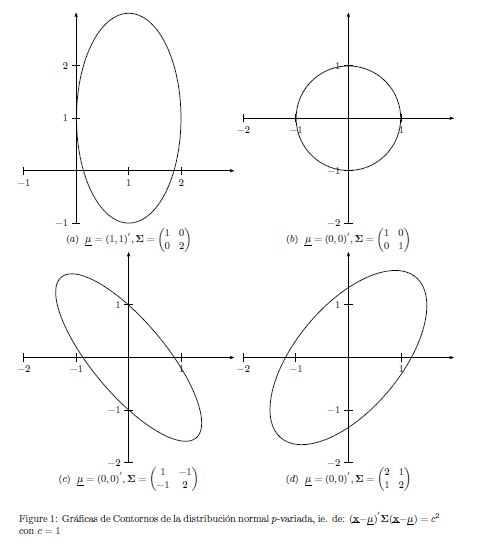
\includegraphics[width=0.5\linewidth]{imagenes/graf59} 

}

\caption{Gráfico de Contornos NM}\label{fig:contornos-prob}
\end{figure}

\begin{theorem}
\protect\hypertarget{thm:teorema-val-vect-prop}{}\label{thm:teorema-val-vect-prop}Si \(\mathbf{\Sigma}\)-es definida-positiva y \(\lambda\) es un valor propio de \(\mathbf{\Sigma}\) asociado al vector propio \(\underline{\mathbf{e}}\) (ie. \(\mathbf{\Sigma} \underline{\mathbf{e}}=\lambda \underline{\mathbf{e}}\)), entonces \(\frac{1}{\lambda}\)-es un valor-propio de \(\mathbf{\Sigma}^{-1}\)-asociado al mismo vector propio \(\underline{\mathbf{e}}\) (ie. \(\mathbf{\Sigma}^{-1} \underline{\mathbf{e}}=\frac{1}{\lambda} \underline{\mathbf{e}}\)). Además, \(\mathbf{\Sigma}^{-1}\)-también es definida positiva.
\end{theorem}

\begin{proof}
Como \(\mathbf{\Sigma}\)-es definida-positiva, se cumple que: \(\underline{\mathbf{e}}^t\mathbf{\Sigma} \underline{\mathbf{e}}>0\), con \(\underline{\mathbf{e}} \neq 0\).

Ahora, para \(\underline{\mathbf{e}}\)-vector-propio de \(\mathbf{\Sigma}\) se cumple lo siguiente:
\[
\mathbf{\Sigma} \underline{\mathbf{e}}=\lambda \underline{\mathbf{e}}, \ \ \text{luego},
\]
\[
0<\underline{\mathbf{e}}^t\mathbf{\Sigma} \underline{\mathbf{e}}=\underline{\mathbf{e}}^t\lambda \underline{\mathbf{e}}=\lambda \underline{\mathbf{e}}^t\underline{\mathbf{e}}=\lambda,
\]
es decir, \(\lambda>0\).

Ahora,
\begin{align*}
\underline{\mathbf{e}}&=\mathbf{\Sigma}^{-1}(\mathbf{\Sigma}\underline{\mathbf{e}})\\
&=\mathbf{\Sigma}^{-1}(\lambda \underline{\mathbf{e}}) \ , \ \ \text{pues} \ \ \mathbf{\Sigma}\underline{\mathbf{e}}=\lambda \underline{\mathbf{e}}\\
\text{luego} \ \ \frac{1}{\lambda}\underline{\mathbf{e}} &= \mathbf{\Sigma}^{-1} \underline{\mathbf{e}},
\end{align*}

es decir, \(\frac{1}{\lambda}\)-es un valor-propio de \(\mathbf{\Sigma}^{-1}\)-asociado al mismo vector propio \(\underline{\mathbf{e}}\).

Veamos que \(\mathbf{\Sigma}^{-1}\)-es Definida positiva. (Def.+).

Para un vector \(\underline{\mathbf{x}}\neq 0\), se cumple lo siguiente:
\begin{align*}
\underline{\mathbf{x}}^t\mathbf{\Sigma}^{-1} \underline{\mathbf{\mathbf{x}}} &= \underline{\mathbf{x}}^t \left( \sum_{i=1}^p \frac{1}{\lambda_i} \underline{\mathbf{e}}_i\underline{\mathbf{e}}_i^t \right) \underline{\mathbf{x}}\ , \ \ \text{por la desc. espectral de} \ \ \mathbf{\Sigma}^{-1}\\
&= \sum_{i=1}^p \frac{1}{\lambda_i} \underline{\mathbf{x}}^t \underline{\mathbf{e}}_i\underline{\mathbf{e}}_i^t  \underline{\mathbf{x}}\\
&= \sum_{i=1}^p \frac{1}{\lambda_i} ( \underline{\mathbf{e}}_i^t \underline{\mathbf{x}})^2\ , \ \text{pues} \ \ (\underline{\mathbf{e}}_i^t \underline{\mathbf{x}})^2= (\underline{\mathbf{e}}_i^t \underline{\mathbf{x}})^t(\underline{\mathbf{e}}_i^t \underline{\mathbf{x}})=\underline{\mathbf{x}}^t \underline{\mathbf{e}}_i\underline{\mathbf{e}}_i^t  \underline{\mathbf{x}}  \\
&>0, \ \ \text{pues los} \ \ \lambda_i>0 \ \ \text{y} \ \ \underline{\mathbf{x}}\neq 0.
\end{align*}

Luego, \(\mathbf{\Sigma}^{-1}\)-es definida positiva.
\end{proof}

\begin{example}[Aspectos Geométricos-1]
\protect\hypertarget{exm:ejemplo-aspectos-geom-1}{}\label{exm:ejemplo-aspectos-geom-1}Suponga que un vector aleatorio \(2\)-dimensional \(\underline{\mathbf{x}}\) tiene la siguiente matriz de Var-Cov,
\[
\mathbf{\Sigma}=\begin{bmatrix}
\sigma_{11} & \sigma_{12}\\
\sigma_{21} & \sigma_{22}
\end{bmatrix}=\begin{bmatrix}
\sigma_{11} & \sigma_{12}\\
\sigma_{21} & \sigma_{11},
\end{bmatrix}
\]
es decir que: \(\sigma_{11}=\sigma_{22}\). Graficar el elipsoide (la elipse) correspondiente bajo la restricción de que \(\rho=Corr(X,Y)>0\). Es decir, dos variables con igual varianza y correlación positiva.
\end{example}

\begin{solution}
Los ejes de la elipse están dados por: \(\pm c \sqrt{\lambda_i} \underline{\mathbf{e}_i}\), para \(i=1,2\) y \(c>0\), es decir: \(\pm c \sqrt{\lambda_1} \underline{\mathbf{e}_1}\) y \(\pm c \sqrt{\lambda_2} \underline{\mathbf{e}_2}\).

Ahora se deben hallar los valores propios de \(\mathbf{\Sigma}\), para lo cual se debe resolver la ecuación característica dada por:
\[
|\mathbf{\Sigma}-\lambda I_2|=0.
\]
\begin{align*}
|\mathbf{\Sigma}-\lambda I_2|&=\left|\begin{pmatrix}
\sigma_{11} & \sigma_{12}\\
\sigma_{12} & \sigma_{11}
\end{pmatrix}-\begin{bmatrix}
\lambda & 0\\
0 & \lambda
\end{bmatrix}\right|\\
&=\left|\begin{matrix}
\sigma_{11}-\lambda & \sigma_{12}\\
\sigma_{12} & \sigma_{11}-\lambda
\end{matrix}\right|\\
&=(\sigma_{11}-\lambda)^2-\sigma_{12}^2\\
&=(\sigma_{11}-\lambda-\sigma_{12})(\sigma_{11}-\lambda+\sigma_{12})
\end{align*}
Al hacer, \((\sigma_{11}-\lambda-\sigma_{12})(\sigma_{11}-\lambda+\sigma_{12})=0\) se obtiene que:
\[
\lambda_1=\sigma_{11}+\sigma_{12}\ \ \ \text{y que}\ \ \  \lambda_2=\sigma_{11}-\sigma_{12}.
\]

Ahora los vectores propios asociados a estos valores propios se obtienen resolviendo la ecuación: \(\mathbf{\Sigma} \underline{\mathbf{e}}=\lambda \underline{\mathbf{e}}\).

Por Ejemplo si,~~
\(\underline{\mathbf{e}}_1=\begin{bmatrix} e_1\\ e_2 \end{bmatrix}\)-es el vector propio asociado al valor propio \(\lambda_1=\sigma_{11}+\sigma_{12}\), entonces debe cumplir que:
\[
\begin{pmatrix}
\sigma_{11} & \sigma_{12} \\
\sigma_{12} & \sigma_{11}
\end{pmatrix} \begin{pmatrix}
e_1 \\ e_2 \end{pmatrix} = (\sigma_{11}+\sigma_{12})\begin{pmatrix}
e_1 \\ e_2 \end{pmatrix},
\]

de donde, se obtiene el siguiente sistema de ecuaciones:
\begin{align*}
\sigma_{11}e_1+\sigma_{12}e_2=(\sigma_{11}+\sigma_{12})e_1 \ \ \Longrightarrow \ \ e_1=e_2\\
\sigma_{12}e_1+\sigma_{11}e_2=(\sigma_{11}+\sigma_{12})e_2 \ \ \Longrightarrow \ \ e_1=e_2
\end{align*}
El vector, \(\underline{\mathbf{e}}_1= \begin{bmatrix} e_1 \\ e_2 \end{bmatrix} = \begin{bmatrix}  e_1 \\ e_1 \end{bmatrix}\)-normalizado está dado por:

\[
\frac{\underline{\mathbf{e}}_1}{\|\underline{\mathbf{e}}_1\|}=\frac{(e_1,e_1)}{\|(e_1,e_1)\|}=\frac{(e_1,e_1)}{\sqrt{2e_1^2}}=\left(\frac{e_1}{e_1\sqrt{2}} , \frac{e_1}{e_1\sqrt{2}}\right)=  \begin{bmatrix}
\frac{1}{\sqrt{2}} \\ \\ \frac{1}{\sqrt{2}}
\end{bmatrix} 
\]
De manera análoga, se encuentra que el segundo vector-propio asociado al segundo valor-propio \(\lambda_2=\sigma_{11}-\sigma_{12}\) es:
\[
\underline{\mathbf{e}}_2^t=\begin{bmatrix}
\frac{1}{\sqrt{2}} \\ \\ -\frac{1}{\sqrt{2}}
\end{bmatrix} 
\]
Ahora, Como \(\rho=\frac{\sigma_{12}}{\sqrt{\sigma_{11}}\sqrt{\sigma_{22}}}>0\), entonces \(\sigma_{12}>0\) y por lo tanto \(\lambda_1>\lambda_2\), pues: ~~\(\lambda_1=\sigma_{11}+\sigma_{12}> \sigma_{11}>\sigma_{11}-\sigma_{12}=\lambda_2\).

De lo anterior se concluye que si \(\sigma_{11}=\sigma_{22}\) y \(\rho >0\), entonces el eje mayor de la elipse está a lo largo de una línea cuya inclinación es de \(45^{°}\) y que pasa por el punto \(\underline{\mu}=(\mu_1,\mu_2)\).
\end{solution}

\begin{figure}

{\centering 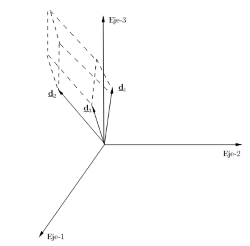
\includegraphics[width=0.5\linewidth]{imagenes/graf6} 

}

\caption{Gráfico de Elipse NB}\label{fig:elipse-NB}
\end{figure}

\begin{example}[Aspectos Geométricos-2]
\protect\hypertarget{exm:ejemplo-aspectos-geom-2}{}\label{exm:ejemplo-aspectos-geom-2}Suponga que el vector aleatorio \(\underline{\mathbf{x}}^t=(X_1,X_2)\) tiene una distribución normal-bivariada, con vector de medias \(\underline{\mu}=(\mu_1,\mu_2)\) y matriz de Var-Cov dada por \(\mathbf{\Sigma}\). Halla la f.d.p multivariada de \(\underline{\mathbf{x}}\).
\end{example}

\begin{solution}
Recordemos que la f.d.p normal bi-variada está dada por:
\[
f(\underline{\mathbf{x}})=(2\pi)^{-\frac{2}{2}}|\mathbf{\Sigma}|^{-\frac{1}{2}}e^{-\frac{1}{2}(\underline{\mathbf{x}}-\underline{\mathbf{\mu}})^t\mathbf{\Sigma}^{-1}(\underline{\mathbf{x}}-\underline{\mathbf{\mu}})}.
\]
Para \(\mathbf{\Sigma}=\begin{bmatrix} \sigma_{11} & \sigma_{12} \\ \sigma_{21} & \sigma_{22} \end{bmatrix}\)

se tiene que:

\(\mathbf{\Sigma}^{-1}=\frac{1}{|\Sigma|}\begin{bmatrix} \sigma_{22} & -\sigma_{12} \\ -\sigma_{12} &\sigma_{11} \end{bmatrix}\),

con \(|\mathbf{\Sigma}|=\sigma_{11}\sigma_{22}-\sigma_{12}^2\), pero \(\sigma_{12}=\rho \sqrt{\sigma_{11}}\sqrt{\sigma_{22}}\),

es decir que, \(|\mathbf{\Sigma}|=\sigma_{11}\sigma_{22}-\rho^2\sigma_{11}\sigma_{22}=\sigma_{11}\sigma_{22}(1-\rho^2)\), de donde:
\[
\mathbf{\Sigma}^{-1}=\frac{1}{\sigma_{11}\sigma_{22}(1-\rho^2)}\begin{bmatrix}
\sigma_{22} & -\sigma_{12} \\ -\sigma_{12} &\sigma_{11}
\end{bmatrix}
\]

Ahora se tiene que:
\begin{align*}
(\underline{\mathbf{x}}-\underline{\mathbf{\mu}})^t\mathbf{\Sigma}^{-1}(\underline{\mathbf{x}}-\underline{\mathbf{\mu}})&=\frac{1}{\sigma_{11}\sigma_{22}(1-\rho^2)}\begin{bmatrix}
x_1-\mu_1 & x_2-\mu_2 
\end{bmatrix}\begin{bmatrix}
\sigma_{22} & -\sigma_{12} \\ -\sigma_{12} &\sigma_{11}
\end{bmatrix}\begin{bmatrix}
x_1-\mu_1 \\ x_2-\mu_2 
\end{bmatrix}\\
&\hspace{-4.5cm}=\frac{1}{\sigma_{11}\sigma_{22}(1-\rho^2)}\sigma_{22}(x_1-\mu_1)^2+\sigma_{11}(x_2-\mu_2)^2-2\rho \sqrt{\sigma_{11}}\sqrt{\sigma_{22}}(x_1-\mu_1)(x_2-\mu_2)\\
&\hspace{-2.0cm}=\frac{1}{1-\rho^2}\left[\left(\frac{x_1-\mu_1}{\sqrt{\sigma_{11}}} \right)^2-2\rho \left(\frac{x_1-\mu_1}{\sqrt{\sigma_{11}}} \right)\left(\frac{x_1-\mu_2}{\sqrt{\sigma_{22}}} \right) +\left(\frac{x_2-\mu_2}{\sqrt{\sigma_{22}}} \right)^2 \right]\\
\end{align*}
de donde,

\[
\frac{1}{2}(\underline{\mathbf{x}}-\underline{\mathbf{\mu}})^t\mathbf{\Sigma}^{-1}(\underline{\mathbf{x}}-\underline{\mathbf{\mu}})=\frac{1}{2(1-\rho^2)}\left[\left(\frac{x_1-\mu_1}{\sqrt{\sigma_{11}}} \right)^2-2\rho \left(\frac{x_1-\mu_1}{\sqrt{\sigma_{11}}} \right)\left(\frac{x_1-\mu_2}{\sqrt{\sigma_{22}}} \right) +\left(\frac{x_2-\mu_2}{\sqrt{\sigma_{22}}} \right)^2 \right]
\]

y como \(|\mathbf{\Sigma}|=\sigma_{11}\sigma_{22}(1-\rho^2)\), entonces
\(|\mathbf{\Sigma}|^{-\frac{1}{2}}=\left[\sigma_{11}\sigma_{22}(1-\rho^2)\right]^{-\frac{1}{2}}\)

por lo tanto,
\begin{align*}
f(\underline{\mathbf{x}})&=f(x_1,x_2)=(2\pi)^{-\frac{2}{2}}|\mathbf{\Sigma}|^{-\frac{1}{2}}e^{-\frac{1}{2}(\underline{\mathbf{x}}-\underline{\mathbf{\mu}})^t\mathbf{\Sigma}^{-1}(\underline{\mathbf{x}}-\underline{\mathbf{\mu}})}\\
& \\
&=(2\pi)^{-1}\left[\sigma_{11}\sigma_{22}(1-\rho^2)\right]^{-\frac{1}{2}}\\
& \\ 
&\hspace{-1.0cm}\text{Exp}\left[-\frac{1}{2(1-\rho^2)}\left[\left(\frac{x_1-\mu_1}{\sqrt{\sigma_{11}}} \right)^2-2\rho \left(\frac{x_1-\mu_1}{\sqrt{\sigma_{11}}} \right)\left(\frac{x_1-\mu_2}{\sqrt{\sigma_{22}}} \right) +\left(\frac{x_2-\mu_2}{\sqrt{\sigma_{22}}} \right)^2 \right] \right]\\
&\\
&=(2\pi)^{-1}\left[\sigma_{11}\sigma_{22}(1-\rho^2)\right]^{-\frac{1}{2}}\\
& \\  
&\hspace{-2.8cm}\text{Exp}\left[-\frac{1}{2(1-\rho^2)}\left(\frac{x_1-\mu_1}{\sqrt{\sigma_{11}}} \right)^2\right]\text{Exp}\left[-\frac{1}{2(1-\rho^2)}\left(\frac{x_2-\mu_2}{\sqrt{\sigma_{22}}} \right)^2\right] \text{Exp}\left[ \frac{\rho}{1-\rho^2} \left(\frac{x_1-\mu_1}{\sqrt{\sigma_{11}}} \right)\left(\frac{x_1-\mu_2}{\sqrt{\sigma_{22}}} \right) \right] 
\end{align*}

Ahora, si las variables \(X_1\) y \(X_2\) tienen \(\rho=0\), entonces:
\begin{align*}
f(\underline{\mathbf{x}})&=f(x_1,x_2)=(2\pi)^{-1}|\mathbf{\Sigma}|^{-\frac{1}{2}}e^{-\frac{1}{2}(\underline{\mathbf{x}}-\underline{\mathbf{\mu}})^t\mathbf{\Sigma}^{-1}(\underline{\mathbf{x}}-\underline{\mathbf{\mu}})}\\
& \\
&=(2\pi)^{-1}\left[\sigma_{11}\sigma_{22}\right]^{-\frac{1}{2}}\text{Exp}\left[-\frac{1}{2} \left(\frac{x_1-\mu_1}{\sqrt{\sigma_{11}}} \right)^2 -\frac{1}{2}\left(\frac{x_2-\mu_2}{\sqrt{\sigma_{22}}} \right)^2 \right]\\
& \\
&\hspace{-1.5cm}=\frac{1}{\sqrt{2\pi}\sqrt{\sigma_{11}}}\text{Exp} \left[-\frac{1}{2} \left(\frac{x_1-\mu_1}{\sqrt{\sigma_{11}}} \right)^2 \right]\frac{1}{\sqrt{2\pi}\sqrt{\sigma_{22}}}\text{Exp} \left[-\frac{1}{2} \left(\frac{x_2-\mu_2}{\sqrt{\sigma_{22}}} \right)^2 \right]\\ \\ 
f(x_1,x_2)&=f(x_1)f(x_2)
\end{align*}
con \(f(x_1)\) la f.d.p de una normal uni-variada con media \(\mu_1\) y varianza \(\sigma_{11}\) y y \(f(x_2)\) la f.d.p de una normal uni-variada con media \(\mu_2\) y varianza \(\sigma_{22}\), ie., si \(\rho=0\) entonces \(X_1\) y \(X_2\) son independientes, pues \(f(x_1,x_2)=f(x_1)f(x_2)\).
\end{solution}

\begin{figure}

{\centering 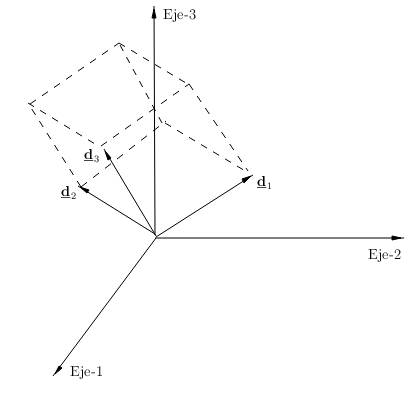
\includegraphics[width=0.5\linewidth]{imagenes/graf7} 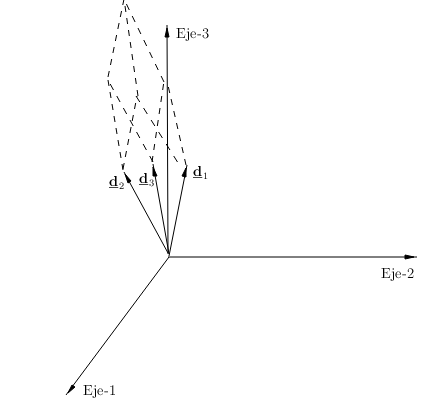
\includegraphics[width=0.5\linewidth]{imagenes/graf8} 

}

\caption{Gráfico de Superficies NB}\label{fig:superficies-NB}
\end{figure}

En el gráfico (a) se observa la superficie (densidad) de una distribución normal-bivarianda con \(\sigma_{11}=\sigma_{22}\) y \(\rho_{12}=Corr(X_1,X_2)=0\)

En el gráfico (b) se observa la superficie (densidad) de una distribución normal-bivarianda con \(\sigma_{11}=\sigma_{22}\) y \(\rho_{12}=Corr(X_1,X_2)=0.75\).

Notar que la presencia de correlación causa que la probabilidad se concentre a lo largo de una línea.

La densidad normal multivariada tiene un máximo valor cuando la distancia cuadrática \((\underline{\mathbf{x}}-\underline{\mathbf{\mu}})^t\mathbf{\Sigma}^{-1}(\underline{\mathbf{x}}-\underline{\mathbf{\mu}})\) es igual a cero, es
decir, cuando \(\underline{\mathbf{x}}=\underline{\mathbf{\mu}}\). Por tanto el punto \(\underline{\mathbf{\mu}}\) es el punto de máxima densidad, o la moda, y también es la media, como se observa en la siguiente gráfica.

\begin{figure}

{\centering 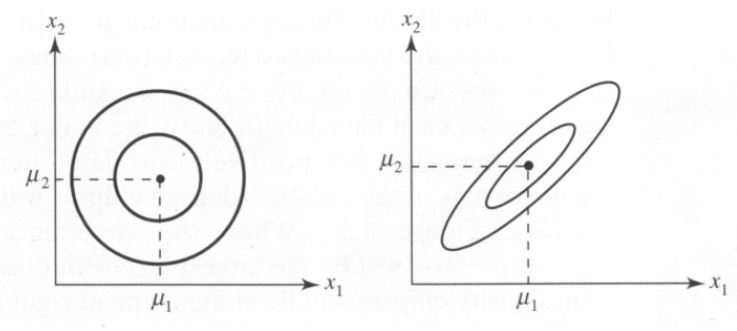
\includegraphics[width=0.65\linewidth]{imagenes/graf9} 

}

\caption{Gráfico de Contornos de Superficies NB}\label{fig:contornos-superficies-NB}
\end{figure}

\hypertarget{propiedades-de-la-distribuciuxf3n-normal-multivariada}{%
\section{Propiedades de la distribución Normal Multivariada}\label{propiedades-de-la-distribuciuxf3n-normal-multivariada}}

Sea \(\underline{\mathbf{x}}\)-un vector aleatorio \(p\)-variado.

\begin{enumerate}
\def\labelenumi{\arabic{enumi}.}
\tightlist
\item
  Si \(\underline{X}\sim N_p(\underline{\mu},\mathbf{\Sigma})\), entonces:
  \begin{equation}
  E[\underline{X}]=\underline{\mu} \  \ \ \text{y}\ \ \ Var[\underline{X}]=\mathbf{\Sigma}
  \label{eq:prop-1}
  \end{equation}
\end{enumerate}

La distribución de \(\underline{X}\)-queda completamente determinada por \(\underline{\mu}\) y \(\mathbf{\Sigma}\).

\begin{enumerate}
\def\labelenumi{\arabic{enumi}.}
\setcounter{enumi}{1}
\tightlist
\item
  Si \(\underline{X}\sim N_p(\underline{\mu},\mathbf{\Sigma})\), entonces
  \begin{equation}
  \underline{a}^t\underline{X}=a_1X_1+a_2X_2+\ldots+a_pX_p \sim N_1(\underline{a}^t\underline{\mu}\ ,\ \underline{a}^t \mathbf{\Sigma} \underline{a})
  \label{eq:prop-2}
  \end{equation}
  Análogamente, si \(\forall \ \underline{a}\in \mathbb{R}^p\) \(\underline{a}^t\underline{X}\sim N_1(\underline{a}^t\underline{\mu}\ ,\ \underline{a}^t \mathbf{\Sigma} \underline{a})\) entonces \(\underline{X}\sim N_p(\underline{\mu},\mathbf{\Sigma})\), es decir:
  \[
  \underline{X}\sim N_p(\underline{\mu},\mathbf{\Sigma}) \Longleftrightarrow \underline{a}^t \underline{X}\sim N_1(\underline{a}^t\underline{\mu}\ ,\ \underline{a}^t \mathbf{\Sigma} \underline{a})
  \]
  Luego, si \(\underline{X}\sim N_p(\underline{\mu},\mathbf{\Sigma})\) entonces cada \(X_i \sim N_1(\mu_i \ , \  \sigma_{ii})\), lo cual se logra con \(\underline{a}=(0,0,\cdots, 1,\cdots, 0,0)^t\) con 1-en la posición \(i\)-ésima del vector \(\underline{a}\) y \(\underline{\mu}\) y \(\mathbf{\Sigma}\) dados por:
  \[
  \mathbf{\underline{\mu}}=\begin{bmatrix}
  \mu_1\\ \mu_2\\ \vdots \\  \mu_p
  \end{bmatrix} \ \ \text{y} \ \ \ \mathbf{\Sigma}=
  \begin{bmatrix}
  \sigma_{11} & \sigma_{12}& \cdots &  \sigma_{1p}\\
  \sigma_{21} & \sigma_{22}& \cdots &  \sigma_{2p}\\
  \vdots & \vdots & \ddots & \vdots\\
  \sigma_{p1}& \sigma_{p2}& \cdots &  \sigma_{pp}
  \end{bmatrix}
  \]
\end{enumerate}

\begin{definition}[Función Generadora de Momentos-NU]
\protect\hypertarget{def:fgm-normal-uni}{}\label{def:fgm-normal-uni}Si una v.a \(X\sim N_1(\mu \, \ \sigma^2)\), entonces la FGM de \(X\) es:
\[
M_X(t):=E[e^{tX}]=e^{\mu t+\frac{1}{2}\sigma^2 t^2}, \ t\in \mathbb{R}
\]
\end{definition}

\begin{definition}[Función Generadora de Momentos-NM]
\protect\hypertarget{def:fgm-normal-multiv}{}\label{def:fgm-normal-multiv}Si un vector aleatorio \(\underline{X}\sim N_p(\underline{\mu},\mathbf{\Sigma})\), entonces la FGM de \(\underline{X}\) es:
\[
M_{\underline{X}}(\underline{t}):=E[e^{\underline{t}^t\underline{X}}]=e^{\underline{t}^t \underline{\mu} +\frac{1}{2}\underline{t}^t  \mathbf{\Sigma}\underline{t}}, \ \ \underline{t} \in \mathbb{R}^p
\]
\end{definition}

\begin{proof}[Desmostración prop.2]
\(\underline{X}\sim N_p(\underline{\mu},\mathbf{\Sigma}) \Longleftrightarrow \underline{a}^t \underline{X}\sim N_1(\underline{a}^t\underline{\mu}\ ,\ \underline{a}^t \mathbf{\Sigma} \underline{a})\)

Sea la v.a \(Y=\underline{a}^t\underline{X}\)
\begin{align*}
M_Y(t)&=E[e^{tY}]=E[e^{t(\underline{a}^t\underline{X})}]\\
&=E[e^{(\underline{a}t)^t\underline{X}}]\ , \ \text{pues} \ \ (\underline{a}t)^t=t^t\underline{a}^t=t\underline{a}^t\\
&=M_{\underline{X}}(\underline{a}t)\\
&=e^{(\underline{a}t)^t\underline{\mu} +\frac{1}{2}(\underline{a}t)^t\mathbf{\Sigma}(\underline{a}t)}\\
&=e^{t^t\underline{a}^t\underline{\mu} +\frac{1}{2}t^t\underline{a}^t\mathbf{ \Sigma} \underline{a}t}\\
&=e^{t(\underline{a}^t\underline{\mu}) +\frac{1}{2}t(\underline{a}^t\mathbf{\Sigma} \underline{a})t}
=e^{t (\underline{a}^t\underline{\mu}) +\frac{1}{2} (\underline{a}^t\mathbf{\Sigma} \underline{a}) t^2}
\end{align*}
es decir, la FGM de \(Y=\underline{a}^t\underline{X}\)-corresponde a la FGM de una v.a normal univariada con media \(\underline{a}^t\underline{\mu}\) y varianza \(\underline{a}^t\mathbf{\Sigma} \underline{a}\), es decir:
\[
Y=\underline{a}^t\underline{X}\sim N_1\left(\underline{a}^t\underline{\mu}\ , \ \underline{a}^t\mathbf{\Sigma} \underline{a}\right), \ \ l.q.q.d
\]
\end{proof}

\begin{example}
\protect\hypertarget{exm:ejemplo-prop-1}{}\label{exm:ejemplo-prop-1}Suponga que \(\underline{\mathbf{x}}\sim N_3 (\underline{\mu} \ , \ \mathbf{\Sigma})\) y considere la combinación linea de las componentes de \(\underline{\mathbf{x}}\) dada por:
\[
\underline{\mathbf{y}}=2X_1-X_2+3X_3=\begin{bmatrix}
2 & -1 & 3
\end{bmatrix}\begin{bmatrix}
X_1 \\ X_2 \\ X_3
\end{bmatrix}=\underline{a}^t\underline{\mathbf{x}}
\]
con \(\underline{a}=\begin{bmatrix} 2 & -1 & 3 \end{bmatrix}^t\), entonces:
\[
E[\underline{\mathbf{y}}]=E[\underline{a}^t\underline{\mathbf{x}}]=
\underline{a}^t \underline{\mu}=\begin{bmatrix}
2 & -1 & 3
\end{bmatrix}\begin{bmatrix}
\mu_1 \\ \mu_2 \\ \mu_3
\end{bmatrix}=2\mu_1-\mu_2+3\mu_3\ , \ \ \text{y}
\]
\begin{align*}
Var[\underline{\mathbf{y}}]&=Var[\underline{a}^t\underline{\mathbf{x}}]\\
&=\underline{a}^t \mathbf{\Sigma} \underline{a}\\
&= \begin{bmatrix}
2 & -1 & 3
\end{bmatrix}\begin{bmatrix}
\sigma_{11} & \sigma_{12} & \sigma_{13}\\
\sigma_{12} & \sigma_{22} & \sigma_{23}\\
\sigma_{13} &\sigma_{23} & \sigma_{33}
\end{bmatrix} \begin{bmatrix}
2 \\ -1 \\ 3
\end{bmatrix}\\
&=\begin{bmatrix}
2\sigma_{11}-\sigma_{12}+3\sigma_{13} & 
2\sigma_{12}-\sigma_{22}+3\sigma_{23} & 
2\sigma_{13}-\sigma_{23}+3\sigma_{33}
\end{bmatrix} \begin{bmatrix}
2 \\ -1 \\ 3
\end{bmatrix}\\
&=4\sigma_{11}-2\sigma_{12}+6\sigma_{13}- 
2\sigma_{12}+\sigma_{22}-3\sigma_{23} +
6\sigma_{13}-3\sigma_{23}+9\sigma_{33}\\
&\\
Var[\underline{\mathbf{y}}]&=4\sigma_{11}
+\sigma_{22}+9\sigma_{33}-4\sigma_{12}+12\sigma_{13}-6\sigma_{23}
\end{align*}
Es decir que:
\[
\underline{\mathbf{y}}=\underline{a}^t\underline{X}=2X_1-X_2+3X_3 \sim N_1(\underline{a}^t\underline{\mu}\ ,\ \underline{a}^t \mathbf{\Sigma} \underline{a}).
\]
con: \(\underline{a}^t \underline{\mu}=2\mu_1-\mu_2+3\mu_3\)~~ y

\(\underline{a}^t \mathbf{\Sigma} \underline{a}= 4\sigma_{11}+\sigma_{22}+9\sigma_{33}-4\sigma_{12}+ 12\sigma_{13}-6\sigma_{23}\).
\end{example}

\begin{enumerate}
\def\labelenumi{\arabic{enumi}.}
\setcounter{enumi}{2}
\tightlist
\item
  Si \(\underline{\mathbf{x}}\sim N_p (\underline{\mu} \ , \ \mathbf{\Sigma})\), entonces
\end{enumerate}

\begin{equation} 
\underline{\mathbf{y}}=A \underline{X}+ \underline{b} \sim N_q(A \underline{\mu}+\underline{b}\ , \ A\mathbf{\Sigma} A^t )
\label{eq:prop-3}
\end{equation}

Si \(\underline{b}=\underline{0}\) se tiene que:
\(\underline{\mathbf{y}}=A \underline{X}\sim N_q(A \underline{\mu}\ , \ A\mathbf{\Sigma} A^t )\), con \(A_{q\times p}\).

\begin{proof}
\begin{align*}
M_{\underline{\mathbf{y}}}(\underline{t})&:=E\left[{\text{ $e^{\underline{t}^t\underline{\mathbf{y}}}$}}\right]=E\left[{\text{ $e^{\underline{t}^t(A\underline{\mathbf{x}}+\underline{b})}$}}\right]\\
&=E\left[{\text{ $e^{\underline{t}^tA\underline{\mathbf{x}}+\underline{t}^t \underline{b}}$}}\right]\\
&=E\left[{\text{ $e^{\underline{t}^tA\underline{\mathbf{x}}} e^{\underline{t}^t \underline{b}}$}}\right]\\
&=\text{ $e^{\underline{t}^t \underline{b}}$}  E\left[{\text{ $e^{\underline{t}^tA\underline{\mathbf{x}}}$}}\right]\\
&=\text{ $e^{\underline{t}^t \underline{b}}$}  E\left[{\text{ $e^{(A^t\underline{t})^t\underline{\mathbf{x}}}$}}\right]\ , \ \text{pues} \ \ (A^t\underline{t})^t=\underline{t}^tA \\
&=\text{ $e^{\underline{t}^t \underline{b}}$}  M_{\underline{X}}(A^t\underline{t})\\
&=\text{ $e^{\underline{t}^t \underline{b}}$}  \left[ \text{ $e^{ (A^t\underline{t})^t \underline{\mu} + \frac{1}{2} (A^t\underline{t})^t \mathbf{\Sigma} (A^t\underline{t})  }$  } \right]
;\ M_{\underline{X}}(\underline{t})=e^{\underline{t}^t\underline{\mu} +\frac{1}{2}\underline{t}^t\mathbf{\Sigma}\underline{t}}\\ 
&= \text{ $e^{\underline{t}^t \underline{b}}$}  \left[ \text{ $e^{ \underline{t}^tA \underline{\mu} + \frac{1}{2} \underline{t}^t A \mathbf{\Sigma} A^t\underline{t}  }$  } \right]\\
&= \text{ $e^{\underline{t}^t  \left( A \underline{\mu} + \underline{b} \right) + \frac{1}{2} \underline{t}^t  \left(A\mathbf{\Sigma} A^t   \right) \underline{t}^t }$} 
\end{align*}

lo cual corresponde a la FGM de un Vector aleatorio normal multivariado con vector de medias \(A \underline{\mu} + \underline{b}\) y matriz de varianzas-covarainzas \(A\mathbf{\Sigma} A^t\), es decir:
\[
\underline{\mathbf{y}}=A \underline{X}+ \underline{b} \sim N_q(A \underline{\mu}+\underline{b}\ , \ A\mathbf{\Sigma} A^t )\ , \ \ l.q.q.d.
\]
\end{proof}

\begin{example}
\protect\hypertarget{exm:ejemplo1-prop-3}{}\label{exm:ejemplo1-prop-3}Suponga que \(\underline{\mathbf{x}}\sim N_3 (\underline{\mu} \ , \ \mathbf{\Sigma})\) y considere el vector de combinaciones lineales de las variables de \(\underline{\mathbf{x}}\) dado por:
\[
\underline{\mathbf{z}}=A\underline{\mathbf{x}}=\begin{bmatrix}
1 & -1 & 0 \\
0 & 1 & -1
\end{bmatrix}\begin{bmatrix}
X_1 \\ X_2\\ X_3
\end{bmatrix}=\begin{bmatrix}
X_1-X_2 \\ X_2 -X_3
\end{bmatrix}=\begin{bmatrix}
Z_1 \\Z_2
\end{bmatrix}
\]
entonces,
\[
\underline{\mathbf{z}}=A \underline{X}\sim N_q(A \underline{\mu}\ , \ A\mathbf{\Sigma} A^t )
\]
donde
\[
A\underline{\mu}=\begin{bmatrix}
1 & -1 & 0 \\
0 & 1 & -1
\end{bmatrix}\begin{bmatrix}
\mu_1 \\ \mu_2\\ \mu_3
\end{bmatrix}=\begin{bmatrix}
\mu_1-\mu_2 \\ \mu_2-\mu_3
\end{bmatrix}=\begin{bmatrix}
E[Z_1] \\ \\ E[Z_2]
\end{bmatrix}
\]
\begin{align*}
A\mathbf{\Sigma} A^t&= \begin{bmatrix}
1 & -1 & 0\\
0 & 1 & -1
\end{bmatrix}\begin{bmatrix}
\sigma_{11} & \sigma_{12} & \sigma_{13}\\
\sigma_{12} & \sigma_{22} & \sigma_{23}\\
\sigma_{13} &\sigma_{23} & \sigma_{33}
\end{bmatrix} \begin{bmatrix}
1 & 0 \\ 
-1 & 1\\
0 & -1
\end{bmatrix}\\ \\ 
&=\begin{bmatrix}
\sigma_{11}-\sigma_{12} & \sigma_{12}-\sigma_{22} & \sigma_{13}-
\sigma_{23}\\
\sigma_{12}-\sigma_{13} & \sigma_{22}-\sigma_{23} & \sigma_{23}-
\sigma_{33}
\end{bmatrix} \begin{bmatrix}
1 & 0 \\ 
-1 & 1\\
0 & -1
\end{bmatrix}\\ \\
&=\begin{bmatrix}
\sigma_{11}-\sigma_{12}-\sigma_{12}+\sigma_{22} & \sigma_{12}-\sigma_{22}-\sigma_{13}+\sigma_{23} \\
\sigma_{12}-\sigma_{13}-\sigma_{22}+\sigma_{23} &  \sigma_{22}-\sigma_{23}-\sigma_{23}+
\sigma_{33}
\end{bmatrix}\\
\\ 
&=\begin{bmatrix}
\sigma_{11}-2\sigma_{12}+\sigma_{22} & \sigma_{12}-\sigma_{22}-\sigma_{13}+\sigma_{23} \\
\sigma_{12}-\sigma_{22}-\sigma_{13}+\sigma_{23} &  \sigma_{22}-2\sigma_{23}+\sigma_{33}
\end{bmatrix}
\end{align*}
\end{example}

\begin{example}
\protect\hypertarget{exm:ejemplo2-prop-3}{}\label{exm:ejemplo2-prop-3}Suponga que \(\underline{\mathbf{x}}^{T}=(X_1,X_2,X_3) \sim N_3(\underline{\mu} \ , \ \mathbf{\Sigma} )\),
donde:
\[
\underline{\mu}=\begin{bmatrix}
2 \\ 1\\ 2
\end{bmatrix} \ ,\ \ \text{y} \ \ \ \Sigma=\begin{bmatrix}
2 & 1 &1 \\
1 & 3 & 0 \\
1 & 0 & 1
\end{bmatrix}
\]
Hallar la distribución conjunta de probabilidad de: \(Z_1=X_1+X_2+X_3\) ~y ~~\(Z_2=X_1-X_2\).
\begin{align*}
\text{Sea}: \ \ \underline{\mathbf{z}}=\begin{bmatrix}
Z_1 \\ Z_2
\end{bmatrix}&=\begin{bmatrix}
X_1+X_2+X_3 \\ X_1-X_2
\end{bmatrix}\\
&=\begin{bmatrix}
1 & 1 &1 \\ 1 & -1 & 0
\end{bmatrix}\begin{bmatrix}
X_1 \\ X_2 \\ X_3
\end{bmatrix}\\
&=A\underline{\mathbf{x}}
\end{align*}
luego,
\[
\underline{\mathbf{z}}=\begin{bmatrix}
Z_1 \\ Z_2
\end{bmatrix} \sim N_2 (A \underline{\mu} \ , \ A\mathbf{\Sigma} A^t),
\]
donde:
\[
A\underline{\mu}= \begin{bmatrix}
1 & 1 &1 \\ 1 & -1 & 0
\end{bmatrix}\begin{bmatrix}
2 \\ 1\\ 2
\end{bmatrix}=\begin{bmatrix}
5 \\ 1
\end{bmatrix}_{2 \times 1}
\]
y
\[
A\mathbf{\Sigma} A^t= \begin{bmatrix}
1 & 1 &1 \\ 1 & -1 & 0
\end{bmatrix}\begin{bmatrix}
2 & 1 &1 \\
1 & 3 & 0 \\
1 & 0 & 1
\end{bmatrix}\begin{bmatrix}
1 & 1\\
1 & -1 \\
1 & 0
\end{bmatrix}=\begin{bmatrix}
4 & 4 &2 \\
1 & -2 & 1
\end{bmatrix}\begin{bmatrix}
1 & 1\\
1 & -1 \\
1 & 0
\end{bmatrix}=\begin{bmatrix}
10 & 0\\
0 & 3 
\end{bmatrix}
\]
de lo anterior, \(Z_1\) y \(Z_2\) son independientes, pues \(Cov(Z_1,Z_2)=0\) y \(Z_1\) y \(Z_2\) son distribuidas normales uni-variadas.
\end{example}

\begin{enumerate}
\def\labelenumi{\arabic{enumi}.}
\setcounter{enumi}{3}
\tightlist
\item
  Sea \(\underline{X}\sim N_p(\underline{\mu},\mathbf{\Sigma})\) y sean los vectores y matrices particionadas dadas por:
  \[
  \underline{\mathbf{x}}=\begin{bmatrix}
  X_1 \\ X_2 \\  \vdots  \\ X_p
  \end{bmatrix}=\begin{bmatrix}
  \underline{\mathbf{x}}^{(1)} \\ \cdots \\ \underline{\mathbf{x}}^{(2)}
  \end{bmatrix} \ \ , \ \ 
  \underline{\mu}=\begin{bmatrix}
  \underline{\mu}^{(1)} \\ \cdots \\ \underline{\mu}^{(2)}
  \end{bmatrix}\ \ \text{y} \ \ 
  \mathbf{\Sigma}_{p\times p}= 
   \begin{bmatrix}
  \mathbf{\Sigma}_{11} & | & \mathbf{\Sigma}_{12} \\
  -- & -- & -- \\
  \mathbf{\Sigma}_{21} & | & \mathbf{\Sigma}_{22}
  \end{bmatrix}
  \]
  entonces:
  \begin{align}
  \underline{\mathbf{x}}^{(1)} & \sim N_q\left(\underline{\mu}^{(1)} \ , \ \mathbf{\Sigma}_{11}\right) \notag  \\ \\
  \underline{\mathbf{x}}^{(2)} & \sim N_{p-q}\left(\underline{\mu}^{(2)} \ , \ \mathbf{\Sigma}_{22}\right).
  \label{eq:prop-4}
  \end{align}
\end{enumerate}

La anterior propiedad también se puede enunciar como sigue: Todos los subconjuntos de variables de \(\underline{\mathbf{x}}\) tienen distribución normal, sea univariada o multivariada.

\begin{proof}
Para esto se usarán las siguientes matrices particionadas:
\[
A_{q\times p}=\begin{array}{cc}
 &\hspace{0.5cm}  q \hspace{1.5cm}  p-q \hspace{1.5cm} \\
 q & \begin{bmatrix}
\hspace{0.5cm} \mathbf{I}_q \hspace{1.0cm} \vdots \hspace{1.0cm} \mathbf{O} \hspace{0.5cm}
 \end{bmatrix}_{q\times p}
\end{array}=\begin{bmatrix}
\hspace{0.5cm} \mathbf{I}_q \hspace{1.0cm} \vdots \hspace{1.0cm} \mathbf{O} \hspace{0.5cm}
 \end{bmatrix}_{q\times p}\ \ \ \ \text{y}\  \ \ \underline{b}=\underline{0}_{q\times 1}
\]
Luego,

\begin{align*}
A\underline{X}+\underline{b}&=A\underline{X}\\
&=\begin{bmatrix}
\hspace{0.5cm} \mathbf{I}_q \hspace{1.0cm} \vdots \hspace{1.0cm} \mathbf{O} \hspace{0.5cm}
 \end{bmatrix}_{q\times p}\begin{bmatrix}
\underline{\mathbf{x}}^{(1)} \\ \cdots \\ \underline{\mathbf{x}}^{(2)}
\end{bmatrix}_{p\times 1} \\
&=\begin{bmatrix}
\hspace{0.5cm} \mathbf{I}_q \ \underline{\mathbf{x}}^{(1)} \hspace{1.0cm} + \hspace{1.0cm} \mathbf{O}\  \underline{\mathbf{x}}^{(2)} \hspace{0.5cm}
 \end{bmatrix}_{q\times 1}\\
 &=\begin{bmatrix}
\hspace{0.5cm} \mathbf{I}_q \ \underline{\mathbf{x}}^{(1)} \hspace{0.5cm}
 \end{bmatrix}_{q\times 1}\\
 &=\begin{bmatrix}
\hspace{0.5cm}  \underline{\mathbf{x}}^{(1)} \hspace{0.5cm}
 \end{bmatrix}_{q\times 1}
\end{align*}
de donde, usando la propiedad \eqref{eq:prop-3} se tiene que:
\[
A\underline{X}+\underline{b}=\underline{\mathbf{x}}^{(1)} \sim N_q(A\underline{\mu}\ , \ A\mathbf{\Sigma} A^t)
\]

Pero,
\begin{align*}
A\underline{\mu}&= \begin{bmatrix}
\hspace{0.5cm} \mathbf{I}_q \hspace{1.0cm} \vdots \hspace{1.0cm} \mathbf{O} \hspace{0.5cm}
 \end{bmatrix} \begin{bmatrix}
\underline{\mu}^{(1)} \\ \cdots \\ \underline{\mu}^{(2)}
\end{bmatrix}\\
&=\begin{bmatrix}
\hspace{0.5cm} \mathbf{I}_q \ \underline{\mu}^{(1)} \hspace{1.0cm} + \hspace{1.0cm} \mathbf{O}\  \underline{\mu}^{(2)} \hspace{0.5cm}
 \end{bmatrix}\\
&=\begin{bmatrix}
\hspace{0.5cm} \mathbf{I}_q \ \underline{\mu}^{(1)}  \hspace{0.5cm}
 \end{bmatrix}\\
&= \begin{bmatrix}
\hspace{0.5cm}  \underline{\mu}^{(1)}  \hspace{0.5cm}
 \end{bmatrix}_{q\times 1}
\end{align*}

\begin{align*}
A\mathbf{\Sigma} A^t&=\begin{bmatrix}
\hspace{0.5cm} \mathbf{I}_q \hspace{1.0cm} \vdots \hspace{1.0cm} \mathbf{O} \hspace{0.5cm}
 \end{bmatrix}\begin{bmatrix}
\mathbf{\Sigma}_{11} & | & \mathbf{\Sigma}_{12} \\
-- & -- & -- \\
\mathbf{\Sigma}_{21} & | & \mathbf{\Sigma}_{22}
\end{bmatrix}\begin{bmatrix}
\mathbf{I}_q \\ \cdots \\   \mathbf{O}  
 \end{bmatrix} \\
 &\\
&=\begin{array}{c}
\begin{bmatrix}
\hspace{0.5cm} \mathbf{I}_q \ \mathbf{\Sigma}_{11}+\mathbf{O}\ \mathbf{\Sigma}_{21}\hspace{1.0cm} \vdots  \hspace{1.0cm} \mathbf{I}_q \ \mathbf{\Sigma}_{12}+\mathbf{O}\ \mathbf{\Sigma}_{22} \hspace{0.5cm}
 \end{bmatrix}\\
 \\ \\
\end{array}  
 \begin{bmatrix}
\mathbf{I}_q \\ \cdots \\   \mathbf{O}  
 \end{bmatrix} \\
&=\begin{array}{c}
\begin{bmatrix}
\hspace{0.5cm}  \mathbf{\Sigma}_{11}+\mathbf{O} \hspace{1.0cm} \vdots  \hspace{1.0cm}  \mathbf{\Sigma}_{12}+\mathbf{O}\ \hspace{0.5cm}
 \end{bmatrix}\\
 \\ \\
\end{array}  
 \begin{bmatrix}
\mathbf{I}_q \\ \cdots \\ \mathbf{O}  
 \end{bmatrix} \\ 
&=\begin{array}{c}
\begin{bmatrix}
\hspace{0.5cm}  \mathbf{\Sigma}_{11} \hspace{1.0cm} \vdots  \hspace{1.0cm}  \mathbf{\Sigma}_{12}\ \hspace{0.5cm}
 \end{bmatrix}\\
 \\ \\
\end{array}  
 \begin{bmatrix}
\mathbf{I}_q \\ \cdots \\ \mathbf{O}  
 \end{bmatrix} \\ 
&=\begin{bmatrix}
\hspace{0.5cm}  \mathbf{\Sigma}_{11} \mathbf{I}_q+ \mathbf{\Sigma}_{12}\mathbf{O}   
\end{bmatrix}\\ \\ 
 &=\begin{bmatrix}
\mathbf{\Sigma}_{11} + \mathbf{O}   
\end{bmatrix}\\ \\ 
& = \mathbf{\Sigma}_{11}
\end{align*}

Es decir que:
\begin{align*}
\underline{\mathbf{x}}^{(1)} & \sim N_q\left(A\underline{\mu}\ , \ A\mathbf{\Sigma} A^t\right)\\
&~  N_q\left(\underline{\mu}^{(1)}\ , \ \mathbf{\Sigma}_{11}\right)\ , \ \ \ \ l.q.q.d.
\end{align*}
\end{proof}

De manera similar, se demuestra que:

\begin{align*}
\underline{\mathbf{x}}^{(2)} & \sim N_q\left(\underline{\mu}^{(2)}\ , \ \mathbf{\Sigma}_{22}\right),
\end{align*}

en este caso usando las matrices particionadas dadas por:
\[
 A=\begin{array}{cc}
 &\hspace{0.5cm}  q \hspace{1.5cm}  p-q \hspace{1.5cm} \\
 p-q & \begin{bmatrix}
\hspace{0.5cm} \mathbf{O} \hspace{1.0cm} \vdots \hspace{1.0cm} \mathbf{I}_{p-q} \hspace{0.5cm}
 \end{bmatrix}_{(p-q)\times p}
\end{array}=\begin{bmatrix}
\hspace{0.5cm} \mathbf{O} \hspace{1.0cm} \vdots \hspace{1.0cm} \mathbf{I}_{p-q} \hspace{0.5cm}
 \end{bmatrix}\ \ ; \ \underline{b}=\underline{0}_{(p-q)\times 1}
\]

\begin{example}
\protect\hypertarget{exm:ejemplo1-prop-4}{}\label{exm:ejemplo1-prop-4}Sea~~\(\underline{\mathbf{x}}\sim N_5 (\underline{\mu} \ , \ \mathbf{\Sigma})\), hallar la distribución de:
\(\begin{bmatrix}X_2 \\ X_4 \end{bmatrix}\).
Sean
\[
\underline{\mathbf{x}}^{(1)}=\begin{bmatrix}
X_2 \\ X_4
\end{bmatrix}\ , \ \ \underline{\mathbf{\mu}}^{(1)}=\begin{bmatrix}
\mu_2 \\ \mu_4 
\end{bmatrix}\ \ \ \text{y} \ \ \ \mathbf{\Sigma}_{11}=\begin{bmatrix}
\sigma_{22} & \sigma_{24}\\
\sigma_{24} & \sigma_{44}
\end{bmatrix}
\]
Asumiendo que \(\underline{\mathbf{x}}\), \(\underline{\mathbf{\mu}}\) y \(\mathbf{\Sigma}\) son particionados como sigue:
\[
\hspace{-2.0cm}\underline{\mathbf{x}}=\begin{bmatrix}
X_2 \\ X_4 \\ \cdots \\ X_1 \\ X_3 \\ X_5
\end{bmatrix}\ , \ \ \underline{\mathbf{\mu}}=\begin{bmatrix}
\mu_2 \\ \mu_4 \\ \cdots \\ \mu_1 \\ \mu_3 \\ \mu_5
\end{bmatrix}\ \ \ \text{y} \ \ \ \mathbf{\Sigma}=\begin{bmatrix}
\sigma_{22} & \sigma_{24} & \vdots & \sigma_{12} & \sigma_{23} & \sigma_{25}\\
\sigma_{24} & \sigma_{44}& \vdots & \sigma_{14} & \sigma_{34} & \sigma_{45}\\
\cdots & \cdots \cdots & \cdots & \cdots & \cdots & \cdots\\
\sigma_{12} &\sigma_{14} & \vdots & \sigma_{11} &\sigma_{13}
&\sigma_{15}  \\
\sigma_{23} &\sigma_{34} & \vdots & \sigma_{13} &\sigma_{33}
&\sigma_{35}  \\
\sigma_{25} &\sigma_{45} & \vdots & \sigma_{15} &\sigma_{35}
&\sigma_{55}  
\end{bmatrix}
\]
\[
\text{es decir}: \ \ \underline{\mathbf{x}}=\begin{bmatrix}
\underline{\mathbf{x}}^{(1)} \\ \cdots \\ \underline{\mathbf{x}}^{(2)}
\end{bmatrix} \ \ , \ \ 
\underline{\mu}=\begin{bmatrix}
\underline{\mu}^{(1)} \\ \cdots \\ \underline{\mu}^{(2)}
\end{bmatrix}\ \ \text{y} \ \ 
\mathbf{\Sigma}= 
 \begin{bmatrix}
\mathbf{\Sigma}_{11} & | & \mathbf{\Sigma}_{12} \\
-- & -- & -- \\
\mathbf{\Sigma}_{21} & | & \mathbf{\Sigma}_{22}
\end{bmatrix}
\]
\[
\text{luego}: \ \ \underline{\mathbf{x}}^{(1)} 
\sim  N_2\left(\underline{\mu}^{(1)}\ , \ \mathbf{\Sigma}_{11}\right)\sim N_2 \left(\begin{bmatrix}
\mu_2 \\ \mu_4 
\end{bmatrix}\ , \begin{bmatrix}
\sigma_{22} & \sigma_{24}\\
\sigma_{24} & \sigma_{44}
\end{bmatrix} \right).
\]
\end{example}

\begin{enumerate}
\def\labelenumi{\arabic{enumi}.}
\setcounter{enumi}{4}
\tightlist
\item
  a).
  \[ 
  \text{Si}, \ \ \ \underline{\mathbf{x}}=\begin{bmatrix}
  \underline{\mathbf{x}}^{(1)} \\ \cdots \\ \underline{\mathbf{x}}^{(2)}
  \end{bmatrix} \sim N_{p} \begin{bmatrix}
  \begin{pmatrix}
  \underline{\mu}^{(1)} \\ \cdots \\ \underline{\mu}^{(2)}
  \end{pmatrix} \ , \ \begin{pmatrix}
  \mathbf{\Sigma}_{11} & | & \mathbf{\Sigma}_{12} \\
  -- & -- & -- \\
  \mathbf{\Sigma}_{21} & | & \mathbf{\Sigma}_{22}
  \end{pmatrix}
  \end{bmatrix}
  \]
  entonces:
  \begin{equation}
  \underline{\mathbf{x}}^{(1)} \perp \underline{\mathbf{x}}^{(2)}\ , \ \ \text{si y solo si} \ \ \mathbf{\Sigma}_{12}=\mathbf{\Sigma}_{21}^t=O_{q\times (p-q)}.
  \label{eq:prop-5a}
  \end{equation}
\end{enumerate}

es decir, \(\underline{\mathbf{x}}^{(1)}\ \ \text{y} \ \ \  \underline{\mathbf{x}}^{(2)}\) son estadísticamente independientes si y solo si:
\(\mathbf{\Sigma}_{12}=\mathbf{\Sigma}_{21}^t=O\).

\begin{example}
\protect\hypertarget{exm:ejemplo1-prop-5}{}\label{exm:ejemplo1-prop-5}Suponga que \(\underline{\mathbf{x}}\sim N_3 (\underline{\mu} \ , \ \mathbf{\Sigma)}\), con
\[
\mathbf{\Sigma}= \begin{bmatrix}
 4 & 1 & 0\\
 1 & 3 & 0 \\
 0 & 0 & 2
\end{bmatrix}
\]
¿Son las variables \(X_1\) y \(X_2\) independientes? Rta. ~~ NO, porque \(\sigma_{12}=1\neq 0\).

¿Son los siguientes vectores aleatorios independientes?:

\(\begin{bmatrix}X_1 \\ X_3 \end{bmatrix}\  \ \text{y} \ \ \begin{bmatrix} X_3 \end{bmatrix}\).

Sean
\[
\underline{\mathbf{x}}=\begin{bmatrix}
X_1 \\ X_2 \\ \cdots \\ X_3
\end{bmatrix}\ , \ \ \underline{\mathbf{\mu}}=\begin{bmatrix}
\mu_1 \\ \mu_2 \\ \cdots \\ \mu_3
\end{bmatrix}\ \ \ \text{y} \ \ \ \mathbf{\Sigma}=\begin{bmatrix}
\sigma_{11} & \sigma_{12} & \vdots & \sigma_{13}\\
\sigma_{21} & \sigma_{22}& \vdots & \sigma_{23}\\
\cdots & \cdots & \cdots & \cdots\\
\sigma_{31} &\sigma_{32} & \vdots & \sigma_{33}
\end{bmatrix}=\begin{bmatrix}
4 & 1 & \vdots & 0\\
1 & 3& \vdots & 0\\
\cdots & \cdots & \cdots & \cdots\\
0 &0 & \vdots & 2
\end{bmatrix}
\]
\[
\text{luego para}:\  \  \ \underline{\mathbf{x}}^{(1)}=\begin{bmatrix}
X_1 \\ X_3
\end{bmatrix}\  \ \text{y} \ \ \underline{\mathbf{x}}^{(2)}=\begin{bmatrix} X_3
\end{bmatrix}
\]
\[
\text{se tiene:} \ \ \ \mathbf{\Sigma}_{12}=Cov\left(\underline{\mathbf{x}}^{(1)}\ , \ \underline{\mathbf{x}}^{(2)}\right)=\begin{bmatrix}
\sigma_{13} \\ \sigma_{23}
\end{bmatrix}=\begin{bmatrix}
0\\0
\end{bmatrix}
\]
por lo tanto, si son independientes.
\end{example}

b). Si \(\underline{\mathbf{x}}^{(1)} \perp \underline{\mathbf{x}}^{(2)}\) ~tales que: ~\\
\(\underline{\mathbf{x}}^{(1)} \sim N_q\left(\underline{\mu}^{(1)}\ , \ \mathbf{\Sigma}_{11}\right) \ \ \ \text{y} \ \ \ \underline{\mathbf{x}}^{(2)} \sim N_q\left(\underline{\mu}^{(2)}\ , \ \mathbf{\Sigma}_{22}\right)\)
entonces,
\begin{equation}
\underline{\mathbf{x}}=\begin{bmatrix}
\underline{\mathbf{x}}^{(1)} \\ \cdots \\ \underline{\mathbf{x}}^{(2)}
\end{bmatrix} \sim N_{p} \begin{bmatrix}
\begin{pmatrix}
\underline{\mu}^{(1)} \\ \cdots \\ \underline{\mu}^{(2)}
\end{pmatrix} \ , \ \begin{pmatrix}
\mathbf{\Sigma}_{11} & | & O \\
-- & -- & -- \\
O & | & \mathbf{\Sigma}_{22}
\end{pmatrix}
\end{bmatrix}
\label{eq:prop-5b}
\end{equation}

c). Si \(\underline{\mathbf{x}}^{(1)} \perp \underline{\mathbf{x}}^{(2)}\) ~, ~\\
\(\underline{\mathbf{x}}^{(1)} \sim N_q\left(\underline{\mu}^{(1)}\ , \ \mathbf{\Sigma}_{11}\right) \ \ \ \text{y} \ \ \ \underline{\mathbf{x}}^{(2)} \sim N_q\left(\underline{\mu}^{(2)}\ , \ \mathbf{\Sigma}_{22}\right)\), Además:
\begin{equation}
\underline{\mathbf{x}}^{(1)}+\underline{\mathbf{x}}^{(2)} \sim N_{k} \left(\underline{\mu}^{(1)}+\underline{\mu}^{(2)} \ , \ \mathbf{\Sigma}_{11}+\mathbf{\Sigma}_{22} \right), \ \ \text{si} \ \ q=p-q=k
\label{eq:prop-5c}
\end{equation}

\begin{proof}
Para esto se usarán la FGM de un vector normal-multivariado dada por:
\[
M_{\underline{X}}(\underline{t}):=E[e^{\underline{t}^t\underline{X}}]={\text{ $e$}}^{\underline{t}^t\underline{\mu} +\frac{1}{2}\underline{t}^t\mathbf{\Sigma}\underline{t}}, \ \ \underline{t} \in \mathbb{R}^p
\]
Sean \(\underline{\mathbf{x}}^{(1)} \perp \underline{\mathbf{x}}^{(2)}\ , \  \underline{\mathbf{x}}^{(1)} \sim N_q\left(\underline{\mu}^{(1)}\ , \ \mathbf{\Sigma}_{11}\right) \ \ \ \text{y} \ \ \ \underline{\mathbf{x}}^{(2)} \sim N_q\left(\underline{\mu}^{(2)}\ , \ \mathbf{\Sigma}_{22}\right)\)

\begin{align*}
M_{\underline{\mathbf{x}}^{(1)}+\underline{\mathbf{x}}^{(2)}}(\underline{t})&:=E\left[e^{\underline{t}^t
\left(\underline{\mathbf{x}}^{(1)}+\underline{\mathbf{x}}^{(2)}\right)} \right]\\
&=E\left[e^{\underline{t}^t\underline{\mathbf{x}}^{(1)}}
e^{\underline{t}^t\underline{\mathbf{x}}^{(2)})} \right]\\
&=E\left[e^{\underline{t}^t\underline{\mathbf{x}}^{(1)}}\right] E\left[
e^{\underline{t}^t\underline{\mathbf{x}}^{(2)})} \right]\ , \ \text{pues}\ \  \ \underline{\mathbf{x}}^{(1)} \perp \underline{\mathbf{x}}^{(2)}\\
&=M_{\underline{\mathbf{x}}^{(1)}}(\underline{t})M_{\underline{\mathbf{x}}^{(2)}}(\underline{t})\\
&={\text{ $e$}}^{\underline{t}^t\underline{\mu}^{(1)} +\frac{1}{2}\underline{t}^t\mathbf{\Sigma}_{11}\underline{t}}{\text{ $e$}}^{\underline{t}^t\underline{\mu}^{(2)} +\frac{1}{2}\underline{t}^t\mathbf{\Sigma}_{22}\underline{t}}\\
&={\text{ $e$}}^{\underline{t}^t\underline{\mu}^{(1)}+{\underline{t}^t\underline{\mu}^{(2)} +\frac{1}{2}\underline{t}^t\mathbf{\Sigma}_{11}\underline{t}} +\frac{1}{2}\underline{t}^t\mathbf{\Sigma}_{22}\underline{t}}\\
&={\text{ $e$}}^{\underline{t}^t \left( \underline{\mu}^{(1)}+\underline{\mu}^{(2)}\right) +\frac{1}{2}\underline{t}^t  \left( \mathbf{\Sigma}_{11}+\mathbf{\Sigma}_{22}\right)\underline{t}}
\end{align*}
lo cual corresponde a la FGM de un vector aleatorio normal multivariado con vector de medias \(\underline{\mu}^{(1)}+\underline{\mu}^{(2)}\) y matriz de varianzas covarianzas \(\mathbf{\Sigma}_{11}+\mathbf{\Sigma}_{22}\), es decir:
\[
\underline{\mathbf{x}}^{(1)}+\underline{\mathbf{x}}^{(2)} \sim N_{k} \left(\underline{\mu}^{(1)}+\underline{\mu}^{(2)} \ , \ \mathbf{\Sigma}_{11}+\mathbf{\Sigma}_{22} \right)\ , \ \ \ l.q.q.d
\]
\end{proof}

Demostración de 5(a) y 5(b); ver Ejercicio 4.14 del libro de Johnson, sixth edition \citep{johnson2007applied}.

\begin{enumerate}
\def\labelenumi{\arabic{enumi}.}
\setcounter{enumi}{5}
\tightlist
\item
  Si
  \(\underline{\mathbf{x}}=\begin{bmatrix} \underline{\mathbf{x}}^{(1)} \\ \cdots \\ \underline{\mathbf{x}}^{(2)} \end{bmatrix} \sim N_{p} \begin{bmatrix} \begin{pmatrix} \underline{\mu}^{(1)} \\ \cdots \\ \underline{\mu}^{(2)} \end{pmatrix} \ , \ \begin{pmatrix} \mathbf{\Sigma}_{11} & | & \mathbf{\Sigma}_{12} \\ -- & -- & -- \\ \mathbf{\Sigma}_{21} & | & \mathbf{\Sigma}_{22} \end{pmatrix} \end{bmatrix},\  \text{con} \  |\mathbf{\Sigma}_{22}|>0\),
\end{enumerate}

entonces, la distribución condicional de \(\underline{\mathbf{x}}^{(1)}\)
dado \(\underline{\mathbf{x}}^{(2)}\) esta dada por:
\begin{equation}
\underline{\mathbf{x}}^{(1)}|\underline{\mathbf{x}}^{(2)}=\underline{\mathbf{x}}^{(2)} \sim N_q \left[ 
\underline{\mu}^{(1)}+\mathbf{\Sigma}_{12}\mathbf{\Sigma}_{22}^{-1}\left(\underline{\mathbf{x}}^{(2)}-
\underline{\mu}^{(2)}\right)  \ , \   \mathbf{\Sigma}_{11}-\mathbf{\Sigma}_{12}\mathbf{\Sigma}_{22}^{-1}\mathbf{\Sigma}_{21}  \right]
\label{eq:prop-6a}
\end{equation}
es decir:
\[
E\left[\underline{\mathbf{x}}^{(1)}|\underline{\mathbf{x}}^{(2)}=\underline{\mathbf{x}}^{(2)}\right]=\underline{\mu}^{(1)}+
\mathbf{\Sigma}_{12}\mathbf{\Sigma}_{22}^{-1}\left(\underline{\mathbf{x}}^{(2)}-
\underline{\mu}^{(2)}\right)
\]
y
\[
Var\left[\underline{\mathbf{x}}^{(1)}|\underline{\mathbf{x}}^{(2)}=\underline{\mathbf{x}}^{(2)}]\right]=
\mathbf{\Sigma}_{11}-\mathbf{\Sigma}_{12}\mathbf{\Sigma}_{22}^{-1}\mathbf{\Sigma}_{21}
\]
De manera similar, si \(|\mathbf{\Sigma}_{11}|>0\), entonces:
\begin{equation}
\underline{\mathbf{x}}^{(2)}|\underline{\mathbf{x}}^{(1)}=\underline{\mathbf{x}}^{(1)} \sim N_{p-q} \left[ \underline{\mu}^{(2)}+\mathbf{\Sigma}_{21}\mathbf{\Sigma}_{11}^{-1}\left(\underline{\mathbf{x}}^{(1)}-
\underline{\mu}^{(1)}\right) \ , \   \mathbf{\Sigma}_{22}-\mathbf{\Sigma}_{21}\mathbf{\Sigma}_{11}^{-1}\mathbf{\Sigma}_{12}  \right]
\label{eq:prop-6b}
\end{equation}

\begin{proof}
Considere la matriz \(p\times p\) dada por:
\[
\mathbf{A}=\begin{bmatrix}
\mathbf{I}_{q\times q} & | & {\mathbf{-\Sigma}_{12}\mathbf{\Sigma}_{22}^{-1}}_{q\times (p-q)} \\
----- & -- & ----- \\
\mathbf{0}_{(p-q)\times q} & | & \mathbf{I}_{(p-q)\times (p-q)}
\end{bmatrix}_{p \times p}
\]
teniendo en cuenta que:
\[
(\underline{X}-\underline{\mu})\sim N_p (\underline{0}\ , \ \mathbf{\Sigma}) 
\]
se tiene que:

\begin{align*}
\underline{Z}_{p\times 1}=\mathbf{A}(\underline{X}-\underline{\mu})&=
\begin{bmatrix}
\mathbf{I}_{q\times q} & | & {\mathbf{-\Sigma}_{12}\mathbf{\Sigma}_{22}^{-1}}_{q\times (p-q)} \\
----- & -- & ----- \\
\mathbf{0}_{(p-q)\times q} & | & \mathbf{I}_{(p-q)\times (p-q)}
\end{bmatrix}\begin{bmatrix}
\underline{X}^{(1)}-\underline{\mu}^{(1)} \\ \\ 
\underline{X}^{(2)}-\underline{\mu}^{(2)} 
\end{bmatrix} \\ \\ 
&=\begin{bmatrix}
\underline{X}^{(1)}-\underline{\mu}^{(1)}{\mathbf{-\Sigma}_{12}\mathbf{\Sigma}_{22}^{-1}}\left(\underline{X}^{(2)}-\underline{\mu}^{(2)}\right)\\ \\ 
\underline{X}^{(2)}-\underline{\mu}^{(2)}
\end{bmatrix} \sim N_p (\underline{\mu}_{\underline{Z}} \ , \ \mathbf{\Sigma}_{\underline{Z}})
\end{align*}
con
\[
\underline{\mu}_{\underline{Z}}=\mathbf{A}\underline{0}=\underline{0}
\]
y
\[
\mathbf{\Sigma}_{\underline{Z}}=\mathbf{A}\mathbf{\Sigma}\mathbf{A}^t
\]
\begin{align*}
\mathbf{A}\mathbf{\Sigma}\mathbf{A}^t&=\begin{bmatrix}
\mathbf{I} & | & {\mathbf{-\Sigma}_{12}\mathbf{\Sigma}_{22}^{-1}} \\
----- & -- & ----- \\
\mathbf{0} & | & \mathbf{I}
\end{bmatrix}\begin{bmatrix}
\mathbf{\Sigma}_{11} & | & \mathbf{\Sigma}_{12} \\
-- & -- & -- \\ 
\mathbf{\Sigma}_{21} & | & \mathbf{\Sigma}_{22}
\end{bmatrix}\mathbf{A}^t \\ \\
& = \begin{bmatrix}
\mathbf{\Sigma}_{11}-\mathbf{\Sigma}_{12}\mathbf{\Sigma}_{22}^{-1}\mathbf{\Sigma}_{21} & | & \mathbf{0} \\
----- & -- & ----- \\
\mathbf{\Sigma}_{21} & | & \mathbf{\Sigma}_{22}
\end{bmatrix} \begin{bmatrix}
\mathbf{I} & | & \mathbf{0}  \\
---- & -- & ---- \\
-\mathbf{\Sigma}_{22}^{-1}\mathbf{\Sigma}_{21}& | & \mathbf{I}
\end{bmatrix} \\ \\ 
&= \begin{bmatrix}
\mathbf{\Sigma}_{11}-\mathbf{\Sigma}_{12}\mathbf{\Sigma}_{22}^{-1}\mathbf{\Sigma}_{21} & | & \mathbf{0} \\
----- & -- & ----- \\
\mathbf{0} & | & \mathbf{\Sigma}_{22}
\end{bmatrix}
\end{align*}

de lo anterior se tiene que como los vectores aleatorios:
\[
\underline{X}^{(1)}-\underline{\mu}^{(1)}{\mathbf{-\Sigma}_{12}\mathbf{\Sigma}_{22}^{-1}}\left(\underline{X}^{(2)}-\underline{\mu}^{(2)}\right) \ \ \ \text{y} \ \ \ 
\underline{X}^{(2)}-\underline{\mu}^{(2)}
\]
tienen matriz de var-cov \(\mathbf{0}\), entonces son independientes, y además se cumple que:
\[
\underline{X}^{(1)}-\underline{\mu}^{(1)}{\mathbf{-\Sigma}_{12}\mathbf{\Sigma}_{22}^{-1}}\left[\underline{X}^{(2)}-\underline{\mu}^{(2)}\right] \sim N_p \left(\underline{\mathbf{0}}\ , \ \mathbf{\Sigma}_{11}-\mathbf{\Sigma}_{12}\mathbf{\Sigma}_{22}^{-1}\mathbf{\Sigma}_{21}\right)
\]
y al ser
\[
\underline{X}^{(1)}-\underline{\mu}^{(1)}{\mathbf{-\Sigma}_{12}\mathbf{\Sigma}_{22}^{-1}}\left(\underline{X}^{(2)}-\underline{\mu}^{(2)}\right) \ \ \ \text{y} \ \ \ 
\underline{X}^{(2)}-\underline{\mu}^{(2)}
\] independientes, entonces la distribución condicional de:
\[
\underline{X}^{(1)}-\underline{\mu}^{(1)}{\mathbf{-\Sigma}_{12}\mathbf{\Sigma}_{22}^{-1}}\left(\underline{X}^{(2)}-\underline{\mu}^{(2)}\right) \ \ \ \text{dado} \ \ \ 
\underline{X}^{(2)}-\underline{\mu}^{(2)}
\]
es igual a la marginal de:
\[
\underline{X}^{(1)}-\underline{\mu}^{(1)}{\mathbf{-\Sigma}_{12}\mathbf{\Sigma}_{22}^{-1}}\left(\underline{X}^{(2)}-\underline{\mu}^{(2)}\right)
\]
cunado \(\underline{X}^{(2)}\) toma un valor fijo, es decir,
\[
\underline{X}^{(1)}|\underline{X}^{(2)}=\underline{X}^{(2)} \sim N_q \left[ \underline{\mu}^{(1)}+\mathbf{\Sigma}_{12}\mathbf{\Sigma}_{22}^{-1}\left(\underline{X}^{(2)}-
\underline{\mu}^{(2)}\right)  \ , \   \mathbf{\Sigma}_{11}-\mathbf{\Sigma}_{12}\mathbf{\Sigma}_{22}^{-1}\mathbf{\Sigma}_{21}  \right]
\]
\end{proof}

\begin{example}
\protect\hypertarget{exm:ejemplo1-prop-6}{}\label{exm:ejemplo1-prop-6}Distribución condicional de una Normal-Bivariada.

Sea \(\underline{\mathbf{x}}=\begin{bmatrix} X_1 \\ X_2 \end{bmatrix} \sim N_{2} \begin{bmatrix} \begin{bmatrix} \mu_{1} \\ \mu_{2} \end{bmatrix} \ , \ \begin{pmatrix} \sigma_{11} & | & \sigma_{12} \\ -- & -- & -- \\ \sigma_{21} & | & \sigma_{22} \end{pmatrix} \end{bmatrix},\  \text{con} \  \sigma_{22}>0\),

luego, la distribución condicional de \(X_1 | X_2\) esta dada por:
\begin{align*}
X_1 | X_2=x_2 & \sim N_1 \left(\mu_1+\frac{\sigma_{12}}{\sigma_{22}}(x_2-\mu_2)\ , \ \sigma_{11}-\frac{\sigma_{12}}{\sigma_{22}}\sigma_{21} \right)
\end{align*}
pues,
\[
\mathbf{\Sigma}_{12}\mathbf{\Sigma}_{22}^{-1}=\sigma_{12}\sigma_{22}^{-1}=\frac{\sigma_{12}}{\sigma_{22}} \ , \ \ \text{y} \ \ 
\]\\
\[
\mathbf{\Sigma}_{11}-\mathbf{\Sigma}_{12}\mathbf{\Sigma}_{22}^{-1}\mathbf{\Sigma}_{21}=\sigma_{11}-
\sigma_{12}\sigma_{22}^{-1}\sigma_{21}=\sigma_{11}-\frac{\sigma_{12}}{\sigma_{22}}\sigma_{21}
\]
y como,

\(\rho_{12}=\frac{\sigma_{12}}{\sqrt{\sigma_{11}}\sqrt{\sigma_{22}}}\), es decir: \(\sqrt{\sigma_{11}}\rho_{12} =\frac{\sigma_{12}}{\sqrt{\sigma_{22}}}\),

luego:
\[
\frac{\sigma_{12}}{\sigma_{22}}=\frac{\sqrt{\sigma_{11}}}{\sqrt{\sigma_{22}}}\rho_{12}
\]
y
\[
\sigma_{11}-\frac{\sigma_{12}}{\sigma_{22}}\sigma_{21}=\sigma_{11}\left[ 1 - \rho_{12}^2\right]
\]
es decir:
\begin{align*}
X_1 | X_2=x_2 & \sim N_1 \left(\mu_1+\frac{\sqrt{\sigma_{11}}}{\sqrt{\sigma_{22}}}\rho_{12}(x_2-\mu_2)\ , \ \sigma_{11}\left[ 1 - \rho_{12}^2\right] \right)\\
& \sim N_1 \left(\underset{a_0}{\underbrace{ \mu_1-\frac{\sqrt{\sigma_{11}}}{\sqrt{\sigma_{22}}}\rho_{12}\mu_2}}+ \underset{b}{\underbrace{\frac{\sqrt{\sigma_{11}}}{\sqrt{\sigma_{22}}}\rho_{12}}}x_2\ , \ \sigma_{11}\left[ 1 - \rho_{12}^2\right] \right)\\
&\\
X_1 | X_2=x_2&\sim N_1 \left(a_0+b x_2\ , \ \sigma_{11}\left[ 1 - \rho_{12}^2\right] \right)
\end{align*}
de donde se observa que la media de la distribución condicional de \(X_1 | X_2=x_2\), corresponde a la ecuación de una línea recta con intecepto \(a_0\) y pendiente \(b\), ie. la ecuación del modelo de regresión lineal de \(X_1\) v.s \(X_2\).
\end{example}

\textbf{Observaciones:}

\begin{itemize}
\item
  En regresión multivariada, la media condicional
  \[
  \underline{\mu}_{1.2}=E[\underline{X}^{(1)} |\underline{X}^{(2)}]
  \]
  es llamada la curva de regresión.
\item
  Entonces la curva de regresión en la normal multivariada, \(\underline{\mu}_{1.2}=E[\underline{X}^{(1)} |\underline{X}^{(2)}]\), se puede escribir como:
  \[
   E[\underline{X}^{(1)} |\underline{X}^{(2)}]=\begin{bmatrix}
  E[X_1 | X_{q+1},X_{q+2},\cdots, X_{p}]\\ \\ 
  E[X_2 | X_{q+1},X_{q+2},\cdots, X_{p}]\\ 
  \vdots  \hspace{3.5cm} \vdots    \\
  \vdots  \hspace{3.5cm} \vdots    \\
  E[X_q | X_{q+1},X_{q+2},\cdots, X_{p}]
  \end{bmatrix}=
  \underline{\mu}^{(1)}+\mathbf{\Sigma}_{12}\mathbf{\Sigma}_{22}^{-1}\left(\underline{X}^{(2)}-
  \underline{\mu}^{(2)}\right) 
  \]
  Ahora sea
  \[
  \mathbf{\Sigma}_{12}\mathbf{\Sigma}_{22}^{-1}=\begin{bmatrix}
  \beta_{1,q+q} & \beta_{1,q+2} & \cdots &\beta_{1,p}\\ \\
  \beta_{2,q+q} & \beta_{2,q+2} & \cdots &\beta_{2,p}\\
  \vdots & \vdots &  & \vdots \\
  \vdots & \vdots &  & \vdots \\
  \beta_{q,q+q} & \beta_{q,q+2} & \cdots &\beta_{q,p}\\
  \end{bmatrix}
  \]
  entonces, la curva de regresión se puede escribir como
  \begin{align*}
   E[\underline{X}^{(1)} |\underline{X}^{(2)}]&=\underline{\mu}^{(1)}+\mathbf{\Sigma}_{12}\mathbf{\Sigma}_{22}^{-1}\left(\underline{X}^{(2)}-
  \underline{\mu}^{(2)}\right)=  \\ \\
  &\begin{bmatrix}
  E[X_1 | X_{q+1},X_{q+2},\cdots, X_{p}]\\ \\ 
  E[X_2 | X_{q+1},X_{q+2},\cdots, X_{p}]\\ 
  \vdots  \hspace{3.5cm} \vdots    \\
  \vdots  \hspace{3.5cm} \vdots    \\
  E[X_q | X_{q+1},X_{q+2},\cdots, X_{p}]
  \end{bmatrix}=\begin{bmatrix}
  \mu_1 \\ \\ \mu_2 \\ \vdots \\ \vdots \\ \mu_q
  \end{bmatrix}+\begin{bmatrix}
  \beta_{1,q+q} & \beta_{1,q+2} & \cdots &\beta_{1,p}\\ \\
  \beta_{2,q+q} & \beta_{2,q+2} & \cdots &\beta_{2,p}\\
  \vdots & \vdots &  & \vdots \\
  \vdots & \vdots &  & \vdots \\
  \beta_{q,q+q} & \beta_{q,q+2} & \cdots &\beta_{q,p}\\
  \end{bmatrix}\begin{bmatrix}
  X_{q+1}- \mu_{q+1}\\ \\ 
  X_{q+2}- \mu_{q+2}\\
  \vdots \\ \vdots \\ 
  X_{p}- \mu_{p}\\
  \end{bmatrix}\\ \\
  &= \begin{bmatrix}
  \mu_1+\beta_{1,q+q}(X_{q+1}- \mu_{q+1}) + \beta_{1,q+2}(X_{q+2}- \mu_{q+2}) + \cdots +\beta_{1,p}(X_{p}- \mu_{p})\\ \\
  \mu_2+\beta_{2,q+q}(X_{q+1}- \mu_{q+1}) + \beta_{2,q+2}(X_{q+2}- \mu_{q+2}) + \cdots +\beta_{2,p}(X_{p}- \mu_{p})\\
  \vdots  \hspace{5.0cm}   \vdots \\
  \vdots \hspace{5.0cm}    \vdots \\
  \mu_q+\beta_{q,q+q}(X_{q+1}- \mu_{q+1}) + \beta_{q,q+2}(X_{q+2}- \mu_{q+2}) + \cdots +\beta_{q,p}(X_{p}- \mu_{p})\\
  \end{bmatrix}
  \end{align*}
\end{itemize}

lo anterior implica que, cuando la distribución conjunta de las variables en una regresión (dependientes e independientes) es normal multivariada, todas las curvas de regresión son lineales.

\begin{itemize}
\tightlist
\item
  La matriz de var-cov condicional
  \[
  \mathbf{\Sigma}_{1.2}=\mathbf{\Sigma}_{11}-\mathbf{\Sigma}_{12}\mathbf{\Sigma}_{22}^{-1}\mathbf{\Sigma}_{21}
  \]
  es constante pues no depende de los valores de las variables condicionantes. Por tanto, la curva de regresión es homocedástica.
\end{itemize}

\begin{example}[Distribución Condicional]
\protect\hypertarget{exm:ejemplo-distrib-condic}{}\label{exm:ejemplo-distrib-condic}Suponga que \(\underline{\mathbf{x}}^{T}=(X_1,X_2,X_3) \sim N_3(\underline{\mu} \ , \ \mathbf{\Sigma} )\), donde:
\[
\underline{\mu}=\begin{bmatrix}
2 \\ 1\\ 2
\end{bmatrix} \ ,\ \ \text{y} \ \ \ \mathbf{\Sigma}=\begin{bmatrix}
2 & 1 &1 \\
1 & 3 & 0 \\
1 & 0 & 1
\end{bmatrix}
\]
Hallar la distribución condicional de: \(\underline{\mathbf{x}}^{(1)} | \underline{\mathbf{x}}^{(2)}\), donde:
\[
\underline{\mathbf{x}}^{(1)}=\begin{bmatrix}
X_1 \\ X_2
\end{bmatrix} \ \ \text{y} \ \ \underline{\mathbf{x}}^{(2)}=\begin{bmatrix} X_3
\end{bmatrix}
\]
La distribución condicional de: \(\underline{\mathbf{x}}^{(1)} | \underline{\mathbf{x}}^{(2)}\) es normal bi-variada con vector de medias:
\[
E[\underline{\mathbf{x}}^{(1)} | \underline{\mathbf{x}}^{(2)} ]=
\underline{\mu}^{(1)}+\mathbf{\Sigma}_{12}\mathbf{\Sigma}_{22}^{-1}\left(\underline{\mathbf{x}}^{(2)}-
\underline{\mu}^{(2)}\right) 
\]
y matriz de var-cov dada por:
\[
Var(\underline{\mathbf{x}}^{(1)} | \underline{\mathbf{x}}^{(2)})=
\mathbf{\Sigma}_{11}-\mathbf{\Sigma}_{12}\mathbf{\Sigma}_{22}^{-1}\mathbf{\Sigma}_{21}
\]
Haciendo,
\[
\underline{\mu}=\begin{bmatrix}
\underline{\mu}^{(1)} \\ \cdots \\ \underline{\mu}^{(2)}
\end{bmatrix}=\begin{bmatrix}
\mu_{1} \\ \mu_2 \\ \cdots \\ \mu_{3}
\end{bmatrix}=\begin{bmatrix}
\begin{pmatrix}
2 \\ 1
\end{pmatrix}
\\ \cdots \\ \begin{pmatrix}
2
\end{pmatrix}
\end{bmatrix}
\]
y
\[
\mathbf{\Sigma}=\begin{bmatrix}
2 & 1 &1 \\
1 & 3 & 0 \\
1 & 0 & 1
\end{bmatrix}=\begin{pmatrix}
\mathbf{\Sigma}_{11} & | & \mathbf{\Sigma}_{12} \\
-- & -- & -- \\
\mathbf{\Sigma}_{21} & | &\mathbf{\Sigma}_{22}
\end{pmatrix}=\begin{bmatrix}
\begin{pmatrix}
2 & 1 \\ 1 & 3
\end{pmatrix} & \vdots & \begin{pmatrix}
1 \\ 0
\end{pmatrix} \\
\cdots & & \cdots \\
\begin{pmatrix}
1 & 0
\end{pmatrix} & \vdots & \begin{bmatrix}
1
\end{bmatrix}
\end{bmatrix}
\]
luego,
\[
E[\underline{\mathbf{x}}^{(1)} | \underline{\mathbf{x}}^{(2)} ]=\underline{\mu}^{(1)}+\mathbf{\Sigma}_{12}\mathbf{\Sigma}_{22}^{-1}\left(\underline{\mathbf{x}}^{(2)}-
\underline{\mu}^{(2)}\right)=\begin{pmatrix}
2 \\1
\end{pmatrix}+\begin{pmatrix}
1 \\ 0
\end{pmatrix} \frac{1}{1}\begin{pmatrix}
x_3-2
\end{pmatrix}=\begin{pmatrix}
x_3 \\ 1
\end{pmatrix}
\]
y
\[
\hspace{-3.0cm} Var(\underline{\mathbf{x}}^{(1)} | \underline{\mathbf{x}}^{(2)})=
\mathbf{\Sigma}_{11}-\mathbf{\Sigma}_{12}\mathbf{\Sigma}_{22}^{-1}\mathbf{\Sigma}_{21}=\begin{pmatrix}
2 & 1 \\ 1 & 3
\end{pmatrix}-\begin{pmatrix}
1 \\ 0
\end{pmatrix}\frac{1}{1}\begin{pmatrix}
1 & 0
\end{pmatrix}=\begin{pmatrix}
1 & 1 \\ 1 & 3
\end{pmatrix}
\]
\end{example}

\begin{enumerate}
\def\labelenumi{\arabic{enumi}.}
\setcounter{enumi}{6}
\tightlist
\item
  Sea \(\underline{X}\sim N_p(\underline{\mu},\mathbf{\Sigma})\). Si \(|\mathbf{\Sigma}|>0\), entonces:
  \begin{equation}
  \underline{\mathbf{z}}=\mathbf{\Sigma}^{-1/2}(\underline{X}-\underline{\mu}) \sim N_p (\underline{0}\ , \ \mathbf{I}_p)
  \label{eq:prop-7}
  \end{equation}
\end{enumerate}

ie, \(\underline{\mathbf{z}}\)-tiene una distribución normal-multivariada estándar.

La Demostración de la propiedad \eqref{eq:prop-7} se puede estudiarla del libro de \citep{johnson2007applied}.

\begin{enumerate}
\def\labelenumi{\arabic{enumi}.}
\setcounter{enumi}{7}
\tightlist
\item
  Sea \(\underline{X}\sim N_p(\underline{\mu},\mathbf{\Sigma})\), con \(|\mathbf{\Sigma}|>0\).
\end{enumerate}

a.)
\begin{equation}
(\underline{X}-\underline{\mu})^t\mathbf{\Sigma}^{-1}(\underline{X}-\underline{\mu})\sim \chi_{p}^2
\label{eq:prop-8a}
\end{equation}

b.) La distribución \(N_p(\underline{\mu}\ , \ \mathbf{\Sigma})\)-asigna probabilidad de \((1-\alpha)100\%\) al elipsoide determinado por:
\begin{equation}
\left\{\underline{\mathbf{x}}\ : \  (\underline{\mathbf{x}} -\underline{\mu})^t\mathbf{\Sigma}^{-1}(\underline{\mathbf{x}} -\underline{\mu}) \leq \chi_{\alpha;p}^2 \right\}
\label{eq:prop-8b}
\end{equation}

donde, \(\chi_{\alpha;p}^2\)-es el percentil superior \(\alpha\) de la distribución \(\chi_p^2\).
\textbackslash end\{enumerate\}

\begin{proof}
Sea
\[
\underline{Z}= \mathbf{\Sigma}^{-1/2} (\underline{X} -\underline{\mu} ),
\]
donde \(\mathbf{\Sigma}^{-1/2}\) es la matriz inversa de \(\mathbf{\Sigma}^{1/2}=\mathbf{\Gamma} \Delta^{1/2}\mathbf{ \Gamma}^{t}\) (llamada la
matriz raíz cuadrada positiva de la matriz \(\mathbf{\Sigma}\)).

entonces, por el resultado de la prop: \eqref{eq:prop-7} se tiene que:
\[
\underline{Z}= \mathbf{\Sigma}^{-1/2} (\underline{X} -\underline{\mu} ) \sim N_p (\underline{0}\ , \ \mathbf{I}_p) 
\]
luego, Las marginales de las variables del vector \(\underline{Z}\) son \(N(0, 1)\) es independientes.

Ahora, se Considera la variable:
\begin{align*}
(\underline{X}-\underline{\mu})^t\mathbf{\Sigma}^{-1}(\underline{X}-\underline{\mu})&=(\underline{X}-\underline{\mu})^t\mathbf{\Sigma}^{-1/2}\mathbf{\Sigma}^{-1/2}(\underline{X}-\underline{\mu}) \\ \\
&=\left(\mathbf{\Sigma}^{-1/2} (\underline{X} -\underline{\mu} ) \right)^t \left(\mathbf{\Sigma}^{-1/2} (\underline{X} -\underline{\mu} ) \right) \\ \\ 
&\hspace{-3.0cm}=\underline{Z}^t\underline{Z} = \sum_{i=1}^p Z_i^2 \sim \chi_{(p)}^2
\end{align*}

\textbf{Observaciones:}

\begin{itemize}
\tightlist
\item
  Por el teorema de descomposición espectral de la
  matriz simétrica y definida positiva \(\mathbf{\Sigma}\)
  \[
  \mathbf{\Sigma}= \mathbf{\Gamma} \mathbf{\Delta} \mathbf{\Gamma}^t
  \]
  donde \(\mathbf{\Gamma}\) es una
  matriz ortogonal con los vectores propios de \(\mathbf{\Sigma}\) como columnas, y \(\mathbf{\Delta}\) es una matriz diagonal con los valores propios de \(\mathbf{\Sigma}\) en su diagonal. Entonces,
  \[
  \mathbf{\Sigma}= \mathbf{\Gamma} \mathbf{\Delta} \mathbf{\Gamma}^t=\mathbf{\Gamma} \mathbf{\Delta}^{1/2}\mathbf{\Delta}^{1/2} \mathbf{\Gamma}^t=(\mathbf{\Gamma} \mathbf{\Delta}^{1/2}\mathbf{\Gamma}^t)(\mathbf{\Gamma}  \mathbf{\Delta}^{1/2} \mathbf{\Gamma}^t)=\mathbf{\Sigma}^{1/2}\mathbf{\Sigma}^{1/2}
  \]
  donde \(\mathbf{\Delta}^{1/2}\) es una matriz diagonal con la raíz cuadrada de los elementos de la diagonal de \(\mathbf{\Delta}\) en su diagonal.
\end{itemize}

A \(\mathbf{\Sigma}^{1/2}=\mathbf{\Gamma} \mathbf{\Delta}^{1/2}\mathbf{\Gamma}^t\) se le llama la
matriz raíz cuadrada positiva de la matriz \(\mathbf{\Sigma}\).

\begin{itemize}
\tightlist
\item
  El empleo de la matriz \(\mathbf{\Sigma}^{-1/2}\) sobre el vector aleatorio \((\underline{X}-\underline{\mu})\) estandariza todas las variables y elimina los efectos de correlación entre ellas.
\end{itemize}

\begin{enumerate}
\def\labelenumi{\arabic{enumi}.}
\setcounter{enumi}{8}
\tightlist
\item
  Sean \(\underline{\mathbf{x}}_1,\underline{\mathbf{x}}_2,\ldots,\underline{\mathbf{x}}_n\), vectores aleatorios \(p\)-variados mutuamente-independientes tales que:
  \[
  \underline{\mathbf{x}}_i \sim N_p (\underline{\mu}_i \ , \ \mathbf{\Sigma})\ , \ \ \text{para} \ \ i=1,2,\ldots,n,
  \]
  entonces:
  \begin{align}
  \underline{\mathbf{v}}_1&=\sum_{i=1}^n c_i\underline{\mathbf{x}}_i \notag \\
  &= c_1\underline{\mathbf{x}}_1+c_2\underline{\mathbf{x}}_2+\cdots+c_n \underline{\mathbf{x}}_n \notag \\
  & \sim N_{p} \left(\sum_{i=1}^n c_i \underline{\mu}_i \ , \ \left( \sum_{}^n c_i^2 \right)\mathbf{\Sigma} \right)\\
  & \sim N_p \left( c_1\underline{\mu}_1+c_2\underline{\mu}_2+\cdots+c_n\underline{\mu}_n \ , \ [c_1^2+c_2^2+\cdots+c_n^2]\mathbf{\Sigma} \right) \notag 
  \label{eq:prop-9a}
  \end{align}
\end{enumerate}

además, si
\[
\underline{\mathbf{v}}_2=\sum_{i=1}^n b_i \underline{\mathbf{x}}_i\\
= b_1\underline{\mathbf{x}}_1+b_2\underline{\mathbf{x}}_2+\cdots+b_n \underline{\mathbf{x}}_n
\]
entonces:
\begin{equation}
\underline{\mathbf{v}}=\begin{bmatrix}
\underline{\mathbf{v}}_1 \\ \cdots \\ \underline{\mathbf{v}}_2
\end{bmatrix} \sim N_{2p} \left[ \begin{pmatrix}
\sum_{i=1}^n c_i \underline{\mathbf{\mu}}_i \\ \cdots\cdots \\ \sum_{i=1}^n b_i \underline{\mathbf{\mu}}_i
\end{pmatrix} \ , \ \mathbf{\Sigma}_{\underline{\mathbf{v}}_1,\underline{\mathbf{v}}_2} \right]\ , \ \ \text{donde}
\label{eq:prop-9b}
\end{equation}

\begin{align*}
\Sigma_{\underline{\mathbf{v}}_1,\underline{\mathbf{v}}_2}=Cov(\underline{\mathbf{v}}_1\ , \ \underline{\mathbf{v}}_2)&=\begin{bmatrix}
\left( \sum_{i=1}^n c_i^2\right) \mathbf{\Sigma} & \vdots &  \left( \sum_{i=1}^n b_ic_i\right) \mathbf{\Sigma} \\
\cdots\cdots & & \cdots\cdots \\
\left( \sum_{i=1}^n b_ic_i\right) \mathbf{\Sigma} & \vdots & \left( \sum_{i=1}^n b_i^2\right) \mathbf{\Sigma}
\end{bmatrix}\\ \\ 
&=\begin{bmatrix}
\left( \underline{c}^t\underline{c} \right) \mathbf{\Sigma} & \vdots &  \left( \underline{b}^t\underline{c} \right) \mathbf{\Sigma} \\
\cdots\cdots & & \cdots\cdots \\
\left( \underline{b}^t\underline{c} \right) \mathbf{\Sigma} & \vdots & \left( \underline{b}^t\underline{b}\right)\mathbf{\Sigma}
\end{bmatrix}_{2p \times 2p}
\end{align*}
y además,~~ \(\underline{\mathbf{v}}_1 \perp \underline{\mathbf{v}}_2\)~~ si ~~ \(\underline{b}^t\underline{c}=\sum_{i=1}^n b_ic_i=0\).
\end{proof}

\begin{proof}
Considere el vector de \(np \times 1\) dado por:
\[
\underline{Z}=\begin{bmatrix}
\underline{X}_1 \\ \underline{X}_2
\\ \vdots \\ \vdots \\ \underline{X}_n\end{bmatrix}_{np\times 1}
\]
por el resultado de la propiedad 5c \eqref{eq:prop-5c} se tiene que:
\[
\underline{Z} \sim N_{np} (\underline{\mu}_{\underline{Z}} \ , \ \mathbf{\Sigma}_{\underline{Z}}) 
\]
donde,
\[
\underline{\mu}_{\underline{Z}}=\begin{bmatrix}
\underline{\mu}_1
\\ \underline{\mu}_2 \\ \vdots \\ \vdots \\ \underline{\mu}_n\end{bmatrix}_{np \times 1} \ \ \ \ \text{y} \ \ \ \ \mathbf{\Sigma}_{\underline{Z}}=\begin{bmatrix}
\mathbf{\Sigma} & \mathbf{0} & \cdots & \mathbf{0}\\
\mathbf{0} & \mathbf{\Sigma} & \cdots & \mathbf{0}\\
\vdots & \vdots &  & \vdots \\
\vdots & \vdots &  & \vdots \\
\mathbf{0} & \mathbf{0} & \cdots &  \mathbf{\Sigma}
\end{bmatrix}_{np \times np}
\]
\end{proof}

\textbf{para la parte (a):}

Considere la matriz
\[
\mathbf{A}=\left[c_1\mathbf{I} \hspace{0.5cm}| \hspace{0.5cm} c_2\mathbf{I}  \hspace{0.5cm}| \hspace{0.5cm} \cdots  \hspace{0.5cm}| \hspace{0.5cm} c_n\mathbf{I} \right]_{p\times np}
\]
donde \(\mathbf{I}\) es la matriz
identidad de orden \(p\times p\), entonces
\[
 \mathbf{A}\underline{Z}=\left[c_1\mathbf{I} \hspace{0.5cm}| \hspace{0.5cm} c_2\mathbf{I}  \hspace{0.5cm}| \hspace{0.5cm} \cdots  \hspace{0.5cm}| \hspace{0.5cm} c_n\mathbf{I} \right]\begin{bmatrix}
\underline{X}_1 \\ \underline{X}_2
\\ \vdots \\ \vdots \\ \underline{X}_n
\end{bmatrix}=c_1\underline{X}_1+c_2\underline{X}_2+\cdots+c_n \underline{X}_n=\underline{V}_1
\]
y por un resultado anterior se tiene que:
\[
 \mathbf{A}\underline{Z}= \underline{V}_1 \sim N_p \left( \mathbf{A} \underline{\mu}_{\underline{Z}} \ , \ \mathbf{A} \mathbf{\Sigma}_{\underline{Z}} \mathbf{A}^t \right)
\]
donde,
\[
\mathbf{A} \underline{\mu}_{\underline{Z}}=\left[c_1\mathbf{I} \hspace{0.5cm}| \hspace{0.5cm} c_2\mathbf{I}  \hspace{0.5cm}| \hspace{0.5cm} \cdots  \hspace{0.5cm}| \hspace{0.5cm} c_n\mathbf{I} \right]\begin{bmatrix}
\underline{\mu}_1 \\ \underline{\mu}_2
\\ \vdots \\ \vdots \\ \underline{\mu}_n
\end{bmatrix}=\sum_{i=1}^n c_i \underline{\mu}_i
\]
y
\begin{align*}
\mathbf{A} \mathbf{\Sigma}_{\underline{Z}} \mathbf{A}^t&= \\
&= \left[c_1\mathbf{I} \hspace{0.5cm}| \hspace{0.5cm} c_2\mathbf{I}  \hspace{0.5cm}| \hspace{0.5cm} \cdots  \hspace{0.5cm}| \hspace{0.5cm} c_n\mathbf{I} \right]\begin{bmatrix}
\mathbf{\Sigma} & \mathbf{0} & \cdots & \mathbf{0}\\
\mathbf{0} & \mathbf{\Sigma} & \cdots & \mathbf{0}\\
\vdots & \vdots &  & \vdots \\
\vdots & \vdots &  & \vdots \\
\mathbf{0} & \mathbf{0} & \cdots &  \mathbf{\Sigma}
\end{bmatrix}\begin{bmatrix}
c_1\mathbf{I} \\ c_2 \mathbf{I} \\ \vdots \\ \vdots \\ c_n \mathbf{I}
\end{bmatrix}  \\ \\ 
& =\begin{bmatrix}
c_1\mathbf{\Sigma} & c_2\mathbf{\Sigma} & \cdots & c_n\mathbf{\Sigma} 
\end{bmatrix}   \begin{bmatrix}
c_1\mathbf{I} \\ c_2 \mathbf{I} \\ \vdots \\ \vdots \\ c_n \mathbf{I}
\end{bmatrix} =  \left( \sum_{i=1}^n c_i^2 \right) \mathbf{\Sigma} \ , \  \ \ \text{es decir},
\end{align*}

\[\underline{\mathbf{v}}_1=\sum_{i=1}^n c_i\underline{X}_i \sim N_p \left( \sum_{i=1}^n c_i \underline{\mu}_i \ , \  \left( \sum_{i=1}^n c_i^2 \right) \mathbf{\Sigma} \right)\ , \ \ \ l.q.q.d
\]

\textbf{para la parte (b):}

Sea
\[
\mathbf{B}=\begin{bmatrix}
 c_1\mathbf{I} \hspace{0.5cm}| \hspace{0.5cm} c_2\mathbf{I}  \hspace{0.5cm}| \hspace{0.5cm} \cdots  \hspace{0.5cm}| \hspace{0.5cm} c_n\mathbf{I} \\ \\ 
  b_1\mathbf{I} \hspace{0.5cm}| \hspace{0.5cm} b_2\mathbf{I}  \hspace{0.5cm}| \hspace{0.5cm} \cdots  \hspace{0.5cm}| \hspace{0.5cm} b_n\mathbf{I}
\end{bmatrix}_{2p \times np} 
\]
entonces
\[
\begin{bmatrix}
\underline{V}_1 \\ \\ \underline{V}_2
\end{bmatrix}= \begin{bmatrix}
c_1\underline{X}_1+c_2\underline{X}_2+\cdots+c_n \underline{X}_n \\ \\
b_1\underline{X}_1+b_2\underline{X}_2+\cdots+b_n \underline{X}_n
\end{bmatrix}=\begin{bmatrix}
 c_1\mathbf{I} \hspace{0.5cm}| \hspace{0.5cm} c_2\mathbf{I}  \hspace{0.5cm}| \hspace{0.5cm} \cdots  \hspace{0.5cm}| \hspace{0.5cm} c_n\mathbf{I} \\ \\ 
  b_1\mathbf{I} \hspace{0.5cm}| \hspace{0.5cm} b_2\mathbf{I}  \hspace{0.5cm}| \hspace{0.5cm} \cdots  \hspace{0.5cm}| \hspace{0.5cm} b_n\mathbf{I}
\end{bmatrix}\begin{bmatrix}
\underline{X}_1 \\ \underline{X}_2 \\ \vdots \\ \vdots \\ \underline{X}_n
\end{bmatrix}=\mathbf{B}\underline{Z}
\]
y de resultados anteriores se tiene que:
\[
\mathbf{B}\underline{Z} \sim N_{2p} \left( \mathbf{B} \underline{\mu}_{\underline{Z}} \ , \ \mathbf{B}\mathbf{\Sigma}_{\underline{Z}} \mathbf{B}^t \right)
\]
donde,
\[
\mathbf{B} \underline{\mu}_{\underline{Z}} = \begin{bmatrix}
 c_1\mathbf{I} \hspace{0.5cm}| \hspace{0.5cm} c_2\mathbf{I}  \hspace{0.5cm}| \hspace{0.5cm} \cdots  \hspace{0.5cm}| \hspace{0.5cm} c_n\mathbf{I} \\ \\ 
  b_1\mathbf{I} \hspace{0.5cm}| \hspace{0.5cm} b_2\mathbf{I}  \hspace{0.5cm}| \hspace{0.5cm} \cdots  \hspace{0.5cm}| \hspace{0.5cm} b_n\mathbf{I}
\end{bmatrix}\begin{bmatrix}
\underline{\mu}_1 \\ \underline{\mu}_2 \\ \vdots \\ \vdots \\ \underline{\mu}_n
\end{bmatrix}=  \begin{bmatrix}
\sum\limits_{=1}^n c_i \underline{\mathbf{\mu}}_i \\ \\ ------ \\ \\  \sum\limits_{=1}^n b_i \underline{\mathbf{\mu}}_i
\end{bmatrix} 
\]
\begin{align*}
 \mathbf{B}\mathbf{\Sigma}_{\underline{Z}} \mathbf{B}^t&=
\begin{bmatrix}
 c_1\mathbf{I} \hspace{0.5cm}| \hspace{0.5cm} c_2\mathbf{I}  \hspace{0.5cm}| \hspace{0.5cm} \cdots  \hspace{0.5cm}| \hspace{0.5cm} c_n\mathbf{I} \\ \\ 
  b_1\mathbf{I} \hspace{0.5cm}| \hspace{0.5cm} b_2\mathbf{I}  \hspace{0.5cm}| \hspace{0.5cm} \cdots  \hspace{0.5cm}| \hspace{0.5cm} b_n\mathbf{I}
\end{bmatrix}
\begin{bmatrix}
\mathbf{\Sigma} & \mathbf{0} & \cdots & \mathbf{0}\\
\mathbf{0} & \mathbf{\Sigma} & \cdots & \mathbf{0}\\
\vdots & \vdots &  & \vdots \\
\vdots & \vdots &  & \vdots \\
\mathbf{0} & \mathbf{0} & \cdots &  \mathbf{\Sigma}
\end{bmatrix}
\begin{bmatrix}
c_1\mathbf{I} & b_1\mathbf{I} \\ c_2\mathbf{I} &b_2 \mathbf{I} \\ \vdots \\ \vdots \\ c_n\mathbf{I} & b_n \mathbf{I}
\end{bmatrix}  
\end{align*}

\begin{align*}
& \mathbf{\Sigma}_{\underline{\mathbf{v}}_1,\underline{\mathbf{v}}_2}=\begin{bmatrix}
 c_1\mathbf{\Sigma} \hspace{0.5cm}| \hspace{0.5cm} c_2\mathbf{\Sigma}  \hspace{0.5cm}| \hspace{0.5cm} \cdots  \hspace{0.5cm}| \hspace{0.5cm} c_n\mathbf{\Sigma} \\ \\ 
  b_1\mathbf{\Sigma} \hspace{0.5cm}| \hspace{0.5cm} b_2\mathbf{\Sigma}  \hspace{0.5cm}| \hspace{0.5cm} \cdots  \hspace{0.5cm}| \hspace{0.5cm} b_n\mathbf{\Sigma}
\end{bmatrix}\begin{bmatrix}
c_1\mathbf{I} & b_1\mathbf{I} \\ c_2\mathbf{I} &b_2 \mathbf{I} \\ \vdots \\ \vdots \\ c_n\mathbf{I} & b_n \mathbf{I}
\end{bmatrix}  \\ \\
& =\begin{bmatrix}
\left( \sum_{i=1}^n c_i^2\right) \mathbf{\Sigma} & \vdots &  \left( \sum_{i=1}^n b_ic_i\right) \mathbf{\Sigma} \\
\cdots\cdots & & \cdots\cdots \\
\left( \sum_{i=1}^n b_ic_i\right) \mathbf{\Sigma} & \vdots & \left( \sum_{i=1}^n b_i^2\right) \mathbf{\Sigma}
\end{bmatrix}=\begin{bmatrix}
\left( \underline{c}^t\underline{c} \right) \mathbf{\Sigma} & \vdots &  \left( \underline{b}^t\underline{c} \right) \mathbf{\Sigma} \\
\cdots\cdots & & \cdots\cdots \\
\left( \underline{b}^t\underline{c} \right) \mathbf{\Sigma} & \vdots & \left( \underline{b}^t\underline{b}\right)\mathbf{\Sigma}
\end{bmatrix}_{2p \times 2p}
\end{align*}

es decir que,
\[
\underline{\mathbf{v}}=\begin{bmatrix}
\underline{\mathbf{v}}_1 \\ \cdots \\ \underline{\mathbf{v}}_2
\end{bmatrix} \sim N_{2p} \left[ \begin{pmatrix}
\sum_{i=1}^n c_i \underline{\mathbf{\mu}}_i \\ \cdots\cdots \\ \sum_{i=1}^n b_i \underline{\mathbf{\mu}}_i
\end{pmatrix} \ , \ \mathbf{\Sigma}_{\underline{\mathbf{v}}_1,\underline{\mathbf{v}}_2} \right]
\]
\textbf{para la parte (c):} Es evidente por resultado de la propiedad 5b \eqref{eq:prop-5b}.

\begin{example}[Distribuciones de CL de Vectores Aleatorios]
\protect\hypertarget{exm:ejemplo-dist-cl-vect-aleat}{}\label{exm:ejemplo-dist-cl-vect-aleat}

Suponga que \(\underline{\mathbf{x}}_1,\underline{\mathbf{x}}_2,\underline{\mathbf{x}}_3,\underline{\mathbf{x}}_4\), son vectores aleatorios \(3\)-variados independientes e idénticamente distribuidos, ie. \(\underline{\mathbf{x}}_i=(X_1,X_2,X_3)^t\), con:
\[
\underline{\mu}=E[\underline{\mathbf{x}}_i]=\begin{bmatrix}
3 \\ -1 \\ 1
\end{bmatrix}\ , \ \ \text{y} \ \ \ \mathbf{\Sigma}=Var[\underline{\mathbf{x}}_i]=\begin{bmatrix}
3 & -1 & 1 \\ -1 & 1 & 0 \\ 1 &0 &2
\end{bmatrix}
\]

\begin{enumerate}
\def\labelenumi{\arabic{enumi}.}
\item
  Hallar la media y varianza de:
  \[
  \underline{a}^t\underline{\mathbf{x}}_1=a_1X_1+a_2X_2+a_3X_3.
  \]
\item
  Hallar la media y varianza de:
  \[
  c_1\underline{\mathbf{x}}_1+c_2\underline{\mathbf{x}}_2+
  c_3\underline{\mathbf{x}}_3+
  c_4\underline{\mathbf{x}}_4=\frac{1}{2}\underline{\mathbf{x}}_1+
  \frac{1}{2}\underline{\mathbf{x}}_2+\frac{1}{2}\underline{\mathbf{x}}_3+\frac{1}{2}\underline{\mathbf{x}}_4
  \]
\item
  Hallar la media y varianza de:
  \[
  \begin{bmatrix}
  c_1\underline{\mathbf{x}}_1+c_2\underline{\mathbf{x}}_2+
  c_3\underline{\mathbf{x}}_3+
  c_4\underline{\mathbf{x}}_4\\  \underline{\mathbf{x}}_1+\underline{\mathbf{x}}_2+
  \underline{\mathbf{x}}_3-3\underline{\mathbf{x}}_4.
  \end{bmatrix}
  \]
\end{enumerate}

\end{example}

\begin{solution}
\leavevmode

\begin{enumerate}
\def\labelenumi{\arabic{enumi}.}
\item
  La distribución de:
  \[
  \underline{a}^t\underline{\mathbf{x}}_1=a_1X_1+a_2X_2+a_3X_3.
  \]
  Una combinación lineal de las componentes de un vector aleatorio, ie. una c.l de variables, lo cual es solo una variable aleatoria, por lo tanto se tiene que:
  \begin{align*}
  E[\underline{a}^t\underline{\mathbf{x}}_1]&=E[a_1X_1+a_2X_2+a_3X_3]\\
  &=a_1E[X_1]+a_2E[X_2]+a_3E[X_3]\\
  &=3a_1-a_2+a_3,
  \end{align*}
  y
  \begin{align*}
  Var[\underline{a}^t\underline{\mathbf{x}}_1]&=Var[a_1X_1+a_2X_2+a_3X_3]\\
  &=a_1^2Var[X_1]+a_2^2Var[X_2]+a_3^2Var[X_3]\\
  &+2a_1a_2Cov(X_1,X_2)+2a_1a_3Cov(X_1,X_3)+
  2a_2a_3Cov(X_2,X_3)\\
  &=3a_1^2+a_2^2+2a_3^2-2a_1a_2+2a_1a_3\\
  &=\underline{a}^t\mathbf{\Sigma} \underline{a}.
  \end{align*}
\item
  La media y varianza de:
  \[
  c_1\underline{\mathbf{x}}_1+c_2\underline{\mathbf{x}}_2+
  c_3\underline{\mathbf{x}}_3+
  c_4\underline{\mathbf{x}}_4=\frac{1}{2}\underline{\mathbf{x}}_1+
  \frac{1}{2}\underline{\mathbf{x}}_2+\frac{1}{2}\underline{\mathbf{x}}_3+\frac{1}{2}\underline{\mathbf{x}}_4
  \]
  En este caso se tiene un combinación lineal de vectores, lo cual a su vez es un vector aleatorio, por lo tanto:
  \begin{align*}
  E[c_1\underline{\mathbf{x}}_1+c_2\underline{\mathbf{x}}_2+
  c_3\underline{\mathbf{x}}_3+
  c_4\underline{\mathbf{x}}_4]&=c_1E[\underline{\mathbf{x}}_1]+
  c_2E[\underline{\mathbf{x}}_2]+c_3E[\underline{\mathbf{x}}_3]+
  c_4E[\underline{\mathbf{x}}_4]\\
  &=\sum_{i=1}^n c_i \underline{\mu}_i\\
  &=c_1\underline{\mu}+c_2\underline{\mu}+c_3\underline{\mu}+
  c_4\underline{\mu}\\
  &=(c_1+c_2+c_3+c_4)\underline{\mu}\\
  &=\left(\frac{1}{2}+\frac{1}{2}+\frac{1}{2}+\frac{1}{2}\right)\underline{\mu}\\
  &=2\underline{\mu}=2\begin{bmatrix}
  3 \\ -1 \\ 1
  \end{bmatrix}=\begin{bmatrix}
  6 \\-2 \\2
  \end{bmatrix}
  \end{align*}
\end{enumerate}

\begin{align*}
Var[c_1\underline{\mathbf{x}}_1+c_2\underline{\mathbf{x}}_2+
c_3\underline{\mathbf{x}}_3+
 c_4\underline{\mathbf{x}}_4]
&=c_1^2Var[\underline{\mathbf{x}}_1]+
c_2^2Var[\underline{\mathbf{x}}_2]+c_3^2Var[\underline{\mathbf{x}}_3]
+c_4^2Var[\underline{\mathbf{x}}_4]\\
&=c_1^2\mathbf{\Sigma}+c_2^2\mathbf{\Sigma}+c_3^2\mathbf{\Sigma}+
c_4^2\mathbf{\Sigma}\\
 &=\left( \sum_{i=1}^n c_i^2 \right)\mathbf{\Sigma}\\
&=(c_1^2+c_2^2+c_3^2+c_4^2)\mathbf{\Sigma}\\
&=\left(\frac{1}{4}+\frac{1}{4}+\frac{1}{4}+\frac{1}{4}\right)\mathbf{\Sigma}\\
&=1 \times \mathbf{\Sigma}\\ 
&=\mathbf{\Sigma}\\
&=\begin{bmatrix}
3 & -1 & 1\\ -1 & 1 &0 \\ 1 & 0& 2
\end{bmatrix}
\end{align*}

\begin{enumerate}
\def\labelenumi{\arabic{enumi}.}
\setcounter{enumi}{2}
\tightlist
\item
  La media y varianza de:
  \[
  \begin{bmatrix}
  c_1\underline{\mathbf{x}}_1+c_2\underline{\mathbf{x}}_2+
  c_3\underline{\mathbf{x}}_3+
  c_4\underline{\mathbf{x}}_4\\ \\  b_1\underline{\mathbf{x}}_1+b_2\underline{\mathbf{x}}_2+
  b_3\underline{\mathbf{x}}_3+b_4\underline{\mathbf{x}}_4
  \end{bmatrix}=\begin{bmatrix}
  \frac{1}{2}\underline{\mathbf{x}}_1+
  \frac{1}{2}\underline{\mathbf{x}}_2+\frac{1}{2}\underline{\mathbf{x}}_3+\frac{1}{2}\underline{\mathbf{x}}_4 \\ \\
  \underline{\mathbf{x}}_1+\underline{\mathbf{x}}_2+
  \underline{\mathbf{x}}_3-3\underline{\mathbf{x}}_4
  \end{bmatrix}=\begin{bmatrix}
  \underline{\mathbf{v}}_1 \\ \\ \underline{\mathbf{v}}_2
  \end{bmatrix}_{6 \times 1}
  \]
\end{enumerate}

Sea\\
\(\underline{\mathbf{v}}=\begin{bmatrix} \underline{\mathbf{v}}_1 \\ \\ \underline{\mathbf{v}}_2 \end{bmatrix}\), luego:

\begin{align*}
Var [\underline{\mathbf{v}}]&= \begin{pmatrix}
Var(\underline{\mathbf{v}}_1) & | & Cov(\underline{\mathbf{v}}_1\ , \ \underline{\mathbf{v}}_2) \\
-- & -- & -- \\
Cov(\underline{\mathbf{v}}_2\ , \ \underline{\mathbf{v}}_1) & | & Var(\underline{\mathbf{v}}_2)
\end{pmatrix}\\
& \\
&=\begin{bmatrix}
\left( \sum_{i=1}^n c_i^2\right) \mathbf{\Sigma}& \vdots &  \left( \sum_{i=1}^n b_ic_i\right) \mathbf{\Sigma} \\
\cdots\cdots & & \cdots\cdots \\
\left( \sum_{i=1}^n b_ic_i\right) \mathbf{\Sigma} & \vdots & \left( \sum_{i=1}^n b_i^2\right)\mathbf{\Sigma}
\end{bmatrix}\\ 
&\\ 
&=\begin{bmatrix}
\left( \underline{c}^t\underline{c} \right) \mathbf{\Sigma} & \vdots &  \left( \underline{b}^t\underline{c} \right) \mathbf{\Sigma} \\
\cdots\cdots & & \cdots\cdots \\
\left( \underline{b}^t\underline{c} \right) \mathbf{\Sigma} & \vdots & \left( \underline{b}^t\underline{b}\right) \mathbf{\Sigma}
\end{bmatrix}_{6 \times 6}\\
&\\ 
&=\begin{bmatrix}
1 \times \mathbf{\Sigma} & \vdots &  0 \times \mathbf{\Sigma} \\
\cdots\cdots & & \cdots\cdots \\
0\times  \mathbf{\Sigma} & \vdots & 12 \times \mathbf{\Sigma}
\end{bmatrix}=\begin{bmatrix}
\mathbf{\Sigma} & \vdots &  \mathbf{0} \\
\cdots\cdots & & \cdots\cdots \\
\mathbf{0} & \vdots & 12\mathbf{\Sigma}
\end{bmatrix}
\end{align*}
es decir,
\[
Var [\underline{\mathbf{v}}]= \begin{bmatrix}
\mathbf{\Sigma} & \vdots &  \mathbf{0} \\
\cdots\cdots & & \cdots\cdots \\
\mathbf{0} & \vdots & 12 \mathbf{\Sigma}
\end{bmatrix}=\begin{bmatrix}
\begin{matrix}
3 & -1 & 1\\ -1 & 1 &0 \\ 1 & 0& 2
\end{matrix} & \vdots &  \begin{matrix}
0 & 0 & 0\\ 0 & 0 &0 \\ 0 & 0& 0
\end{matrix} \\
\cdots\cdots & & \cdots\cdots \\
\begin{matrix}
0 & 0 & 0\\ 0 & 0 &0 \\ 0 & 0& 0
\end{matrix} & \vdots & \begin{matrix}
36 & -12 & 12\\ -12 & 12 &0 \\ 12 & 0& 24
\end{matrix}
\end{bmatrix}
\]

\end{solution}

\textbf{Observaciones:}

\begin{itemize}
\item
  Cada componente de la primera combinación lineal es
  independiente de cada componente de la segunda
  combinación lineal.
\item
  Conjuntamente las dos combinaciones lineales tienen una
  distribución normal multivariada 6-dimensional.
\item
  Las dos combinaciones lineales son independientes.
\end{itemize}

\begin{align*}
\underline{\mathbf{v}}=\begin{bmatrix}
\underline{\mathbf{v}}_1 \\ \\ \underline{\mathbf{v}}_2
\end{bmatrix}&=\begin{bmatrix}
\frac{1}{2}\underline{\mathbf{x}}_1+
\frac{1}{2}\underline{\mathbf{x}}_2+\frac{1}{2}\underline{\mathbf{x}}_3+\frac{1}{2}\underline{\mathbf{x}}_4 \\ \\
\underline{\mathbf{x}}_1+\underline{\mathbf{x}}_2+
\underline{\mathbf{x}}_3-3\underline{\mathbf{x}}_4
\end{bmatrix}\\ \\
&= \begin{bmatrix}
\frac{1}{2}(\underline{\mathbf{x}}_1+
\underline{\mathbf{x}}_2+\underline{\mathbf{x}}_3+
\underline{\mathbf{x}}_4) \\ \\
\underline{\mathbf{x}}_1+\underline{\mathbf{x}}_2+
\underline{\mathbf{x}}_3-3\underline{\mathbf{x}}_4
\end{bmatrix}\\ \\
&=\begin{bmatrix}
\frac{1}{2}\begin{pmatrix}
X_{11} \\ X_{12} \\ X_{13}
\end{pmatrix}+\frac{1}{2}
\begin{pmatrix}
X_{21} \\ X_{22} \\ X_{23}
\end{pmatrix}+\frac{1}{2}\begin{pmatrix}
X_{31} \\ X_{32} \\ X_{33}
\end{pmatrix}+\frac{1}{2}
\begin{pmatrix}
X_{41} \\ X_{42} \\ X_{43}
\end{pmatrix} \\ \\
\begin{pmatrix}
X_{11} \\ X_{12} \\ X_{13}
\end{pmatrix}+\begin{pmatrix}
X_{11} \\ X_{12} \\ X_{13}
\end{pmatrix}+
\begin{pmatrix}
X_{11} \\ X_{12} \\ X_{13}
\end{pmatrix}-3\begin{pmatrix}
X_{11} \\ X_{12} \\ X_{13}
\end{pmatrix}
\end{bmatrix}
\end{align*}

\[
\underline{\mathbf{v}}=\begin{bmatrix}
\underline{\mathbf{v}}_1 \\ \\\underline{\mathbf{v}}_2
\end{bmatrix}=\begin{bmatrix}
\frac{1}{2} \left(X_{11} + X_{21} + X_{31}+X_{41} \right) \\ 
\\
\frac{1}{2} \left(X_{12} + X_{22} + X_{32} +X_{42} \right)\\ 
\\
\frac{1}{2} \left(X_{13} + X_{23} + X_{33} + X_{43}\right)\\
\cdots \cdots \cdots \cdots \cdots \cdots \cdots \cdots \cdots \cdots  
\\
X_{11} + X_{21} + X_{31}-3X_{41} \\
\\
X_{12} + X_{22} + X_{32} -3X_{42}  \\ 
\\
X_{13} + X_{23} + X_{33} -3X_{43}
\end{bmatrix}
\]
\[
\mathbf{\Sigma}_{\underline{\mathbf{x}}_i}=\begin{bmatrix}
3 & -1 & 1\\ -1 & 1 &0 \\ 1 & 0& 2
\end{bmatrix}
\]
\[
\mathbf{\Sigma}_{\underline{\mathbf{v}}}=\begin{bmatrix}
\begin{matrix}
3 & -1 & 1\\ -1 & 1 &0 \\ 1 & 0& 2
\end{matrix} & \vdots &  \begin{matrix}
0 & 0 & 0\\ 0 & 0 &0 \\ 0 & 0& 0
\end{matrix} \\
\cdots\cdots & & \cdots\cdots \\
\begin{matrix}
0 & 0 & 0\\ 0 & 0 &0 \\ 0 & 0& 0
\end{matrix} & \vdots & \begin{matrix}
36 & -12 & 12\\ -12 & 12 &0 \\ 12 & 0& 24
\end{matrix}
\end{bmatrix}
\]

\hypertarget{evaluaciuxf3n-del-supuesto-de-normalidad-multivariada}{%
\section{Evaluación del Supuesto de Normalidad Multivariada}\label{evaluaciuxf3n-del-supuesto-de-normalidad-multivariada}}

Evaluar el supuesto de normalidad multivariada es importante para facilitar los procesos de inferencia estadística.

Existen varios métodos o alternativas para evaluar el supuesto de normalidad multivariada de un vector aleatorio.

Cuando \(n\)-es grande y los métodos de evaluación utilizados se basan en el vector de medias muestrales \(\overline{\underline{\mathbf{x}}}\) o en ciertas distancias que involucran dicho vector de medias muestrales, el supuesto de normalidad multivariada parece no ser tan crucial.

En este caso la calidad de las inferencias realizadas, dependerá de qué tan parecida sea la distribución del vector de medias muestrales \(\overline{\underline{\mathbf{x}}}\) a una normal multivariada.

También es importante tener métodos para identificar cuando la distribución de un vector aleatorio se aleja de la normal multivariada, y así tener cuidado con los análisis posteriores.

\textbf{Propiedad de la Normal-Multivariada}

Recordar que bajo el supuesto de normalidad multivariada de un vector aleatorio \(\underline{\mathbf{x}}_{p\times 1}\), cualquier combinación lineal de las componentes de dicho vector tiene una distribución normal univariada.

Los gráficos de contorno de la normal tri-variada son elipsoides (o hiperelipsoides) y para el caso particular de \(p=2\) (normal bi-variada) son elipses.

\textbf{Preguntas Adecuadas:}

Algunos pasos previos antes de evaluar la normalidad multivariada, corresponden a responder las siguientes preguntas:

\begin{enumerate}
\def\labelenumi{\arabic{enumi}.}
\item
  ¿Son las distribuciones marginales del vector aleatorio, parecídas a normales univariadas?
\item
  ¿Es la distribución de alguna combinación lineal de las componentes de \(\underline{\mathbf{x}}_{p\times 1}\), NO parecida a una normal univariada?
\item
  ¿Al hacer gráficos de dispersión por pares de componentes de
  \(\underline{\mathbf{x}}_{p\times 1}\), presentan algunos de ellos comportamientos no elípticos?
\item
  ¿Existen datos atípicos a nivel marginal o a nivel bivariado?
\end{enumerate}

\textbf{Métodos prácticos:}

En la práctica para evaluar el supuesto de normalidad multivariado, generalmente se procede analizando la normalidad de las marginales del vector \(\underline{\mathbf{x}}_{p\times 1}\) y analizando la normalidad bivariada de pares de componentes de dicho vector.

No es frecuente, en la práctica, encontrar conjuntos de datos normales en bajas dimensiones (ie, \(p=1\) o \(p=2\)) y que no lo sean en altas dimensiones, pero hay que tener en cuenta que \textbf{la normalidad univariada no implica la normalidad multivariada}, ver un ejemplo en el EJERCICIO 4.8 de \citep{johnson2007applied}, un caso de normalidad univariadas que no implica Normalidad-bi-variada.

\hypertarget{evaluaciuxf3n-a-nivel-marginal-ie.-normalidad-univariada}{%
\subsection{Evaluación a nivel marginal (ie. Normalidad Univariada)}\label{evaluaciuxf3n-a-nivel-marginal-ie.-normalidad-univariada}}

gds fdg fdg

  \bibliography{bibliografia/book.bib,bibliografia/packages.bib}

\backmatter
\printindex

\end{document}
